\documentclass[a4paper,11pt,dvipsnames, twocolumn]{article}
\usepackage[a4paper,left=2cm,right=2cm,top=2.5cm,bottom=2.5cm]{geometry}

\usepackage[utf8]{inputenc}
\usepackage[spanish]{babel}
\usepackage{amsmath}
\usepackage{enumerate}
\usepackage{caption}
\usepackage{graphicx}
\usepackage{xcolor}

\usepackage[locale=FR, per-mode=fraction, separate-uncertainty=true]{siunitx}
\usepackage{physics}
\ExplSyntaxOn
\msg_redirect_name:nnn { siunitx } { physics-pkg } { none }
\ExplSyntaxOff

\usepackage{stackengine}  % Needed for colorsection.
\usepackage[most]{tcolorbox}  % Needed for colorsection.
\usepackage[lastexercise,answerdelayed]{exercise}
\usepackage{multicol}  % Respuestas en dos columnas.

\usepackage{circuitikz,pgfplots}  %pgfplots needed for axis environment.
\usepackage{tikz-3dplot}
\usetikzlibrary{babel}  % Solves the problems produced by changes to category codes made by some babel modules.
\usetikzlibrary{decorations, decorations.pathmorphing}
\usetikzlibrary{shapes.geometric}
\usetikzlibrary{arrows, arrows.meta}
\usetikzlibrary{calc}
\usetikzlibrary{patterns}
\usetikzlibrary{3d}  % Babinet.

\newcommand{\anio}{2024}
\newcommand{\comision}{2\textsuperscript{do} 31}

% Imprimir lista de ejercicios seleccionados para hacer en clase.
\newcommand{\seleccionados}{false}


\renewcommand{\thefigure}{\arabic{section}.\arabic{figure}}
\renewcommand{\theequation}{\arabic{section}.\arabic{equation}}

\renewcommand\spanishtablename{Tabla}


%---------------------------
%
% Section headers with colors.
%
%---------------------------
% \usepackage{stackengine}
% \usepackage[most]{tcolorbox}

\definecolor{topcolor}{RGB}{0,121,138}


% \newcommand{\colorofsection}{cyan!90!white}
\newcommand{\colorofsection}{topcolor}
\newcommand{\colorsection}[1]{
    \tcbset{on line,
        boxsep=5pt, left=0pt,right=0pt,top=0pt,bottom=0pt,
        colframe=white, colback=\colorofsection, sharp corners=southwest,
        leftrule=0pt, highlight math style={enhanced}
        }

    \refstepcounter{section}%
    \bigskip\bigskip
    {\noindent\def\stackalignment{l}%
    \stackunder[-2pt]{\tcbox{\textcolor{white}{\textbf{\Large\thesection.\hspace{5pt}#1}}}}{\textcolor{\colorofsection}{\rule{\linewidth}{1pt}}}\medskip}
    \addcontentsline{toc}{section}{\thesection\hspace{5pt}#1}
}

%---------------------------
%
% Exercises and answers.
%
%---------------------------
% \usepackage[lastexercise,answerdelayed]{exercise}
% \usepackage{multicol}
\counterwithin{Exercise}{section}
\renewcommand{\ExerciseHeader}{
    \noindent\textbf{\large
    \ExerciseHeaderNB\ExerciseHeaderTitle
    \ExerciseHeaderOrigin}}
\renewcommand{\AnswerHeader}{\noindent\medskip{\textbf{\ExerciseHeaderNB\hspace{5pt}}}}

%---------------------------
%
% Tikz
%
%---------------------------

\tikzset{axis/.style={blue, thick,-latex}}

% Optica:
% \newcommand\planemirror{} % just for safety
\def\planemirror[#1](#2)(#3)(#4)(#5){%
  % Synopsis
  % \planemirror[fill options](center)(length)(angle)(thickness)
  \fill[#1]   (#2) + ({-0.5*#3*cos(#4)},{-0.5*#3*sin(#4)})
  --++ ({0.5*#3*cos(#4)},{0.5*#3*sin(#4)})
  --++ ({#5*sin(#4)},{-#5*cos(#4)}) --++ ({-#3*cos(#4)},{-#3*sin(#4)}) -- cycle;
  \draw (#2) + ({-#3*cos(#4)/2},{-#3*sin(#4)/2}) --++ ({0.5*#3*cos(#4)},{0.5*#3*sin(#4)});
}
% \newcommand\ray{} % just for safety
\def\ray(#1)(#2)(#3)(#4){%
  % Synopsis
  % \ray[](starting point)(end point)(position of arrow)(xscale)
  \draw[red, thick] (#1) -- (#2) node[color=red, currarrow, pos=#3, xscale=#4, sloped] {};
}

%---------------------------
%
% Babinet
%
%---------------------------

\newcommand{\object}[1]{%
	\begin{scope}[canvas is xz plane at y=1.2]
		\draw[line join=round, thick, fill=black!40] (#1,-1.2) rectangle (#1+0.1,1.2);
	\end{scope}
	%
	\begin{scope}[canvas is xy plane at z=1.2]
		\draw[line join=round, thick, fill=black!25](#1,-1.2) rectangle (#1+0.1,1.2);
	\end{scope}
	%
	\begin{scope}[canvas is yz plane at x=#1]
		\draw[line join=round, thick, fill=black] (-1.2,-1.2) rectangle (1.2,1.2);
		\draw[line join=round, thick, fill=white] (0,0.3) -- (0.3,-0.15) -- (-0.3,-0.15) -- cycle;
		\draw[line join=round, thick, fill=black!40] (0.04,0.24) -- (-0.1667,-0.07) -- (0.2467,-0.07) -- (0.3,-0.15) -- (-0.3,-0.15) -- (0,0.3) -- cycle;
		\draw[thick] (-0.3,-0.15) -- (-0.1667, -0.07);
	\end{scope}
}
\newcommand{\objecttriangle}[1]{%
	\begin{scope}[canvas is yz plane at x=#1]
		\draw[line join=round, thick, fill=black] (0,0.3) -- (0.3,-0.15) -- (-0.3,-0.15) -- cycle;
		\draw[line join=round, thick, fill=black!40] (0,0.3) -- (0.1333, 0.38) -- (0.4333,-0.07)
		-- (0.3,-0.15) -- cycle;
	\end{scope}
}
\newcommand{\image}[1]{%
	\def\point{0.3}
	\def\inside{0.15}
	\begin{scope}[canvas is yz plane at x=#1]
		\draw[line join=round, thick, fill=black] (-1.2,-1.2) rectangle (1.2,1.2);
		\draw[line join=round, thick, fill=red] (0,\point) -- (\inside*0.5,\inside*0.707) -- (\point*0.707,\point*0.5) -- (\inside,0) -- (\point*0.707, -\point*0.5) -- (\inside*0.5, -\inside*0.707) -- (0,-\point) -- (-\inside*0.5, -\inside*0.707) -- (-\point*0.707, -\point*0.5) -- (-\inside,0) -- (-\point*0.707,\point*0.5) -- (-\inside*0.5,\inside*0.707) -- cycle;
	\end{scope}
}
\newcommand{\lens}[1]{%
	\begin{scope}[canvas is yz plane at x=#1+0.1]
		\draw[cyan!30] (0,0) circle (30pt);
	\end{scope}
	\begin{scope}[canvas is yz plane at x=#1]
		\shade[left color=cyan!0,right color=cyan!30]
		(0,0) circle (30pt);
		\draw[cyan!30] (0,0) circle (30pt);
	\end{scope}
}
%---------------------------


%---------------------------
%
% Genera una lista dinámica con
% ejercicios seleccionados.
%
%---------------------------

\let\svaddtocontents\addtocontents
\makeatletter
\newcommand\defineList[1]{%
 \expandafter\def\csname add#1line\endcsname##1##2##3{\addtocontents {##1}{%
  \protect \csname #1line\endcsname {##2}{##3}}}
 \expandafter\def\csname write#1\endcsname{%
  \renewcommand\addtocontents[2]{\relax}%
  \setcounter{section}{0}\noindent%
  \expandafter\def\csname #1line\endcsname####1####2{\expandafter\csname####1\endcsname{####2}}%
  \@starttoc{#1}%
  \setcounter{section}{0}%
  \let\addtocontents\svaddtocontents%
 }%
 \csname add#1line\endcsname{#1}{begin}{itemize}%
 \AtEndDocument{\csname add#1line\endcsname{#1}{end}{itemize}}
}
\newcommand\addToList[2]{\csname add#1line\endcsname{#1}{item}{#2}}
\newcommand\printList[1]{\csname write#1\endcsname}
\makeatother

%---------------------------


% \includeonly{termo_portada.code, termo_dilatacion.code, termo_calorimetria.code,
%   termo_preguntas_calorimetria.code, termo_transmision.code,
%   termo_preguntas_transmision.code, termo_primerppio.code,
%   termo_segundoppio.code, termo_preguntas_principios.code,
%   termo_adicionales.code}


\graphicspath{{./electrodinamica/img/}}

\pgfplotsset{compat=1.18}

\begin{document}

  \setcounter{section}{18}

  % \begin{titlepage}
% \begin{figure}[ht]
\begin{center}
\vspace{1.5cm}
% Aquí se inserta el escudo o emblema:
\begin{tikzpicture}[scale=1, every node/.style={scale=1}]
    % \definecolor{topcolor}{RGB}{15,130,17};
    % \definecolor{botcolor}{RGB}{15,130,17};
    \definecolor{topcolor}{RGB}{0,121,138}
    \definecolor{botcolor}{RGB}{0,96,154};


    \fill[color=topcolor] (1.8273,1.065) arc (30.235:149.765:2.115) -- cycle;
    \fill[color=botcolor] (1.8273,-1.065) arc (-30.235:-149.765:2.115) -- cycle;

    \draw[color=botcolor, thick] (-1.755,-0.625) -- (1.755, -0.625);
    \fill[color=botcolor] (-1.755,-0.0929) -- (1.755, -0.0929) -- (1.755, -0.5405) -- (-1.755,-0.5405) -- cycle;

    % \fill [black](0,-0.7) circle(2pt);

    % \draw (-1.7539,0.93) rectangle (-0.9592,0);
    \fill[] (-1.7539,0.93) arc (180:360:0.39735) -- (-1.1178,0.93) arc (360:180:0.23875) -- cycle;
    \fill[] (-1.7539,0) arc (180:0:0.39735) -- (-1.1178,0) arc (0:180:0.23875) -- cycle;
    \fill (-1.7539,0.3866) rectangle (-0.9592,0.5434);
    \fill (-1.43495,0.93) rectangle (-1.27815,0);

    \fill[color=topcolor] (-0.7795,0.3275) arc[start angle=180, end angle=360,x radius=0.40585, y radius=0.3275] -- (0.0322,0.8506) arc[start angle=0, end angle=180,x radius=0.08925, y radius=0.0794] -- (-0.1463,0.3275) arc[start angle=0, end angle=-180,x radius=0.22735, y radius=0.1604] -- (-0.603, 0.8506) arc[start angle=0, end angle=180,x radius=0.08925, y radius=0.0794] -- cycle;

    \fill[color=topcolor] (0.4003,0.0794) arc[start angle=180, end angle=360,x radius=0.08925, y radius=0.0794] -- (0.5788,0.7515) -- (0.7986,0.7515) arc[start angle=-90, end angle=90,x radius=0.0794, y radius=0.08925] -- (0.1805,0.93) arc[start angle=90, end angle=270,x radius=0.0794, y radius=0.08925] -- (0.4003, 0.7515) -- cycle;

    \fill[color=topcolor] (0.9455,0.0794) arc[start angle=180, end angle=360,x radius=0.08925, y radius=0.0794] -- (1.124,0.608) -- (1.57,0.0267) arc[start angle=-153.217, end angle=0,x radius=0.09411, y radius=0.07059] -- (1.755,0.8506) arc[start angle=0, end angle=180,x radius=0.08925, y radius=0.0794] -- (1.5765,0.3191) -- (1.124,0.9004) arc[start angle=26.783, end angle=180,x radius=0.09411, y radius=0.07059] -- cycle;

    \node [scale=0.8,color=white] at (-1.3822,-0.31) {{\fontfamily{cmss}\selectfont \textbf{A}}};
    \node [scale=0.8,color=white] at (-1.0751,-0.31) {{\fontfamily{cmss}\selectfont \textbf{V}}};
    \node [scale=0.8,color=white] at (-0.768,-0.31) {{\fontfamily{cmss}\selectfont \textbf{E}}};
    \node [scale=0.8,color=white] at (-0.4609,-0.31) {{\fontfamily{cmss}\selectfont \textbf{L}}};
    \node [scale=0.8,color=white] at (-0.1536,-0.31) {{\fontfamily{cmss}\selectfont \textbf{L}}};
    \node [scale=0.8,color=white] at (0.1536,-0.31) {{\fontfamily{cmss}\selectfont \textbf{A}}};
    \node [scale=0.8,color=white] at (0.4605,-0.31) {{\fontfamily{cmss}\selectfont \textbf{N}}};
    \node [scale=0.8,color=white] at (0.7676,-0.31) {{\fontfamily{cmss}\selectfont \textbf{E}}};
    \node [scale=0.8,color=white] at (1.0749,-0.31) {{\fontfamily{cmss}\selectfont \textbf{D}}};
    \node [scale=0.8,color=white] at (1.3822,-0.31) {{\fontfamily{cmss}\selectfont \textbf{A}}};

    \node [scale=1] at (0,-0.845) {{\fontfamily{cmss}\selectfont UDB Física}};

\end{tikzpicture}

\end{center}
% \end{figure}

\begin{center}
    {\LARGE UNIVERSIDAD TECNOLÓGICA NACIONAL}\par\medskip
    \vspace*{0.25cm}
    {\LARGE Facultad Regional Avellaneda}\par\medskip
    \vspace*{1cm}
    {\Huge Física II - \comision}\par\medskip
    \vspace*{0.5cm}
    {\LARGE Guía de problemas de la unidad III}\par\bigskip
    \vspace*{1cm}
    {\Huge \bf \color[RGB]{0,121,138} Campo Eléctrico y Campo Magnético\par\medskip}
\end{center}

\vspace{1cm}

% \newpage
% \pagenumbering{roman}
\begin{center}
    \begin{minipage}[t]{.7\textwidth}
        \renewcommand*{\contentsname}{Contenidos}
        \tableofcontents
    \end{minipage}
    \vspace*{\fill}
\end{center}
\begin{center}
    Año \anio
\end{center}

\end{titlepage}

% \newpage
% \section*{Palabras de bienvenida, a manera de prólogo}
% \addcontentsline{toc}{section}{Prólogo}

% En esta guía de problemas hay material suficiente como para entrenarse en la resolución de problemas prácticos. Además de éstos, las guías contienen problemas gráficos y teóricos. Los primeros ayudan a entender el comportamiento e interrelación entre las propiedades físicas más allá de lo que dicen las fórmulas y los familiarizan con un procedimiento que será rutinario en su vida profesional. Por su parte, en los problemas teóricos (indicados con el marcador \textbf{\raisebox{.5pt}{\textcircled{\raisebox{-1.2pt} {T}}}}) se presentan los fundamentos necesarios para conceptualizar el tema en cuestión. No es obligatorio resolverlos ni estudiar de memoria su resolución, aunque sí recomendamos que los lean detenidamente, pues especifican las definiciones y aproximaciones aplicadas de cada concepto, las cuales resultan necesarias para determinar el contexto de los problemas.
% \par

% \newpage

% \section*{Bibliografía}
% \addcontentsline{toc}{section}{Bibliografía}

% Si bien hay numerosos textos que tratan sobre los temas de la materia, lamentablemente no hay una bibliografía adecuada que contenga todos los temas de este curso al nivel que se presentan, por lo que no hay una bibliografía oficial para la materia. Con los apuntes de clase y algunas notas que se encuentran en IOL ya tienen una base suficiente para cubrir los temas. Sin embargo, si quieren recurrir a fuentes adicionales para complementarlas están los siguientes libros, tradicionales de los cursos de ingeniería:

% \begin{itemize}%\reducespace
% \item \textit{Física para la ciencia y la tecnología}. Tipler y Mosca, 6\textsuperscript{a} edición, capítulos 14-16 y 31-33.
% \item \textit{Fundamentos de física}. Halliday y Resnick, 8\textsuperscript{a} edición, capítulos 15-17 y 33-36.
% \item \textit{Física para ciencias e ingeniería}. Serway y Jewett, 8\textsuperscript{a} edición, capítulos 15-17 y 35-38.
% \item \textit{Física universitaria}. Sears, Zemansky, Young y Freedman, 11\textsuperscript{a} edición.
% \end{itemize}

\newpage
\pagenumbering{arabic}

  % % \begin{center}
%   {\scshape \Huge  Campo Eléctrico\par}
%  \end{center}
%  \vspace{0.5 cm}

\colorsection{Campo eléctrico de cargas puntuales}
\setcounter{figure}{0}

\begin{Exercise}
  Una carga puntual de $\SI{-8.0}{\nano\coulomb}$ se localiza en el origen de un sistema de coordenadas. Obtenga el vector campo eléctrico en la posición $\va*{r} = \SI{1.2}{\metre}\vu{i} - \SI{1.6}{\metre}\vu{j}$.
\end{Exercise}
\begin{Answer}
  $\va*{E} = \SI{-10.8}{\newton/\coulomb}\vu{i} + \SI{14.4}{\newton/\coulomb}\vu{j}$
\end{Answer}
%
\begin{Exercise}
Una partícula $\alpha$ es el núcleo de un átomo de helio, que tiene una masa de $\SI{6.64E-27}{\kilogram}$ y una carga eléctrica de $\SI{3.20E-19}{\coulomb}$. Compare la fuerza de la repulsión eléctrica entre dos partículas $\alpha$ con la fuerza de atracción gravitatoria que hay entre ellas, calculando el cociente $F_e/F_g$.
\end{Exercise}
\begin{Answer}
  $F_e/F_g = 3.1\times 10^{35}$
\end{Answer}
%
\begin{Exercise}
Dos cargas puntuales se localizan en el eje $+x$ de un sistema de coordenadas. La carga $q_1 = \SI{1.0}{\nano\coulomb}$ está a $\SI{2.0}{\centi\metre}$ del origen, y la carga $q_2 = \SI{-3.0}{\nano\coulomb}$ está a $\SI{4.0}{\centi\metre}$ del origen. ¿Cuál es la fuerza total que ejercen estas dos cargas sobre una carga $q_3 = \SI{5.0}{\nano\coulomb}$ que se encuentra en el origen?
\end{Exercise}
\begin{Answer}
  $\va*{F} = \SI{-2.8E-5}{\newton}\vu{i}$
\end{Answer}
%
\begin{Exercise}\label{p:puntuales01}
  Tres cargas puntuales, $q_1$, $q_2$ y $q_3$, están equiespaciadas a lo largo de una recta horizontal, como muestra la figura \ref{f:puntuales01}. Si $q_1 = Q$ y $q_2 = -Q$, ¿cuánto deberá valer $q_3$ para que la fuerza neta sobre $q_1$ sea cero?
\end{Exercise}
\begin{Answer}
  $q_3 = 4Q$
\end{Answer}
%
\begin{center}
  \begin{tikzpicture}[scale=0.8]
    \draw [blue] (0,0)--(6,0);
    \fill [black](1,0) circle(4pt) node[above] {$q_1$};
    \fill [black](3,0) circle(4pt) node[above] {$q_2$};
    \fill [black](5,0) circle(4pt) node[above] {$q_3$};
  \end{tikzpicture}
  \captionof{figure}{Problema \ref{p:puntuales01}\label{f:puntuales01}}
\end{center}
%
\begin{Exercise}
  Tres cargas puntuales están alineadas a lo largo del eje $x$. La carga $q_1 = \SI{3.00}{\micro\coulomb}$ está en el origen, la carga $q_2 = \SI{-5.00}{\micro\coulomb}$ se encuentra en $x = \SI{0.200}{\metre}$, y la tercera carga es $q_3 = \SI{-8.00}{\micro\coulomb}$. ¿Dónde está situada $q_3$ si la fuerza neta sobre $q_1$ es $\SI{7.00}{\newton}$ en la dirección negativa del eje $x$?
\end{Exercise}
\begin{Answer}
  $x = \SI{-0.144}{\metre}$
\end{Answer}
%
\begin{Exercise}
  Considerar la siguiente distribución de cargas: $q_1 = \SI{1}{\milli\coulomb}$ en la posición $\va*{r}_1 = (\SI{0}{\metre};\SI{0}{\metre})$; $q_2 = \SI{3}{\milli\coulomb}$ en la posición $\va*{r}_2 = (\SI{2}{\metre};\SI{0}{\metre})$ y $q_3 = \SI{-2}{\milli\coulomb}$ en la posición $\va*{r}_3 = (\SI{0}{\metre};\SI{1}{\metre})$. Calcular el módulo y el ángulo de la fuerza $\va*{F}_1$ que la distribución ejerce sobre la carga $q_1$.
\end{Exercise}
\begin{Answer}
  \begin{minipage}[t]{.5\textwidth}
    $|\va*{F}_1| = \SI{19.2}{\kilo\newton}$\\ $\theta = \SI{110.6}{\degree}$
  \end{minipage}
\end{Answer}
%
\begin{Exercise}
  Se tienen cuatro cargas puntuales idénticas, de carga $q$, ubicadas en los vértices de un cuadrado de $\SI{20}{\centi\metre}$ de lado. \textit{a}) Calcular la fuerza que sentirá una carga puntual $2q$ situada en el centro del cuadrado. \textit{b}) Calcular la fuerza que actúa sobre esa carga central cuando se quita una de las cargas de los vértices.
\end{Exercise}
\begin{Answer}
  \begin{minipage}[t]{.5\textwidth}
    \textit{a}) $F = 0$\\ \textit{b}) $F = 100kq^2\si{\metre^{-2}}$
  \end{minipage}
\end{Answer}
%
\begin{minipage}[t]{.6\textwidth}
\begin{Exercise}\label{p:puntuales02}
  Dos pequeñas esferas igualmente cargadas y de la misma masa están suspendidas de un mismo punto por dos hilos no conductores de igual longitud $l = \SI{15}{\centi\metre}$, como se muestra en la figura \ref{f:puntuales02}. Debido a la repulsión, el equilibrio se establece cuando las dos esferas están separadas una distancia $d = \SI{10}{\centi\metre}$. Calcular la carga $q$ de cada esfera si la masa de cada esfera es $m = \SI{0.5}{\gram}$.
\end{Exercise}
\begin{Answer}
  $|q| = \SI{44}{\nano\coulomb}$
\end{Answer}
\end{minipage}
%
\begin{minipage}[t]{.4\textwidth}
\strut\vspace*{-\baselineskip}
\begin{center}
  \begin{tikzpicture}[scale=0.2]
    \draw [blue] (0,0)--(6,0);
    \draw [blue] (0,0)--(0.5,1);
    \draw [blue] (0.5,0)--(1,1);
    \draw [blue] (1,0)--(1.5,1);
    \draw [blue] (1.5,0)--(2,1);
    \draw [blue] (2,0)--(2.5,1);
    \draw [blue] (2.5,0)--(3,1);
    \draw [blue] (3,0)--(3.5,1);
    \draw [blue] (3.5,0)--(4,1);
    \draw [blue] (4,0)--(4.5,1);
    \draw [blue] (4.5,0)--(5,1);
    \draw [blue] (5,0)--(5.5,1);
    \draw [blue] (5.5,0)--(6,1);
    \draw [blue] (3,0)--(-2,-14.14) node[black,midway,left] {$l$};
    \fill [black](-2,-14.14) circle(10pt) node[left] {$q$};
    \draw [blue] (3,0)--(8,-14.14) node[black, midway,right] {$l$};
    \fill [black](8,-14.14) circle(10pt) node[right] {$q$};
    \draw [black, {Stealth}-{Stealth}] (-2,-15)--(8,-15) node[black,midway,above] {$d$};
  \end{tikzpicture}
  \captionof{figure}{Problema \ref{p:puntuales02}\label{f:puntuales02}}
\end{center}
\end{minipage}
%
\begin{Exercise}\label{p:puntuales03}
Las cargas $q_1 = \SI{2}{\micro\coulomb}$, $q_2 = \SI{-8}{\micro\coulomb}$ y $q_3 = \SI{12}{\micro\coulomb}$ se colocan en los vértices de un triángulo equilátero, cuyos lados miden $\SI{10}{\centi\metre}$, como se muestra en la figura \ref{f:puntuales03}. \textit{a}) Hallar el campo eléctrico en el punto $P$. \textit{b}) Hallar la fuerza sobre una carga de $\SI{-1}{\micro\coulomb}$ si es colocada en $P$.
\end{Exercise}
\begin{Answer}
  \begin{minipage}[t]{.4\textwidth}
    \textit{a}) $\va*{E} = ( -36\vu{i} + 9.6\vu{j} )\times 10^6 \si{\newton/\coulomb}$\\ \textit{b}) $\va*{F} = ( 36\vu{i} - 9,6\vu{j} )\si{\newton}$
  \end{minipage}
\end{Answer}
%
\begin{minipage}[t]{.5\textwidth}
% \strut\vspace*{-\baselineskip}
\begin{center}
  \begin{tikzpicture}[scale=0.3]
    \draw [blue, dashed] (0,0)--(-5,-8.66);
    \draw [blue, dashed] (0,0)--(5,-8.66);
    \draw [blue, dashed] (-5,-8.66)--(5,-8.66);
    \draw [blue, dashed] (0,0)--(0,-8.66);
    \fill [black](-5,-8.66) circle(10pt) node[left] {$q_1$};
    \fill [black](0,0) circle(10pt) node[left] {$q_2$};
    \fill [black](5,-8.66) circle(10pt) node[right] {$q_3$};
    \fill [red](0,-8.66) circle(10pt) node[above right] {$P$};
  \end{tikzpicture}
  \captionof{figure}{Problema \ref{p:puntuales03}\label{f:puntuales03}}
\end{center}
\end{minipage}
%
\begin{minipage}[t]{.5\textwidth}
\begin{center}
  \begin{tikzpicture}[scale=0.6]
    \draw [blue, dashed] (0,0)--(4,0);
    \draw [blue, dashed] (0,0)--(0,4);
    \draw [blue, dashed] (0,4)--(4,4);
    \draw [blue, dashed] (4,0)--(4,4);
    \fill [black](0,0) circle(5pt) node[left] {$2q$};
    \fill [black](0,4) circle(5pt) node[left] {$q$};
    \fill [black](4,0) circle(5pt) node[right] {$-4q$};
    \fill [black](4,4) circle(5pt) node[right] {$2q$};
  \end{tikzpicture}
  \captionof{figure}{Problema \ref{p:puntuales04}\label{f:puntuales04}}
\end{center}
\end{minipage}
%
\begin{Exercise}\label{p:puntuales04}
  Calcule el módulo del campo eléctrico resultante en el centro de un cuadrado de lado $b$, en cuyos vértices se sitúan las cargas $q$, $2q$, $-4q$ y $2q$, como se muestra en la figura \ref{f:puntuales04}.
\end{Exercise}
\begin{Answer}
  $|\va*{E}| = 10kq/b^2$
\end{Answer}
%
\begin{Exercise}\label{p:puntuales05}
  Dos cargas se colocan como se muestra en la figura \ref{f:puntuales05}. La carga $q_1$ vale $\SI{3.00}{\milli\coulomb}$ y se desconocen el signo y el valor de la carga $q_2$. El campo eléctrico neto en el punto $P$ está por completo en la dirección horizontal hacia la derecha, como se observa en la figura. Calcular el módulo del vector campo eléctrico en el punto $P$.
\end{Exercise}
\begin{Answer}
  $|\va*{E}| = \SI{2.8E10}{\newton/\coulomb}$
\end{Answer}
%
\begin{Exercise}\label{p:puntuales06}
  Sobre el eje $x$ se ubican una carga positiva $q$ en la posición $x = d/2$ y una carga negativa $-q$ en la posición $x = -d/2$, como se observa en la figura \ref{f:puntuales06}. De esta forma se tiene un dipolo eléctrico de separación $d$, cuyo momento dipolar es $\va*{p}=qd\vu{x}$, paralelo al eje $x$. Este dipolo se encuentra en una región donde existe un campo eléctrico uniforme que forma un ángulo de $30^\circ$ con el eje $x$. \textit{a}) ¿Cuál es la fuerza neta que ejerce el campo externo sobre el dipolo? \textit{b}) Calcular el torque que siente este dipolo ($\va*{\tau} = \va*{p} \times \va*{E}$) si $q = \SI{12}{\nano\coulomb}$, $d = \SI{5}{\centi\metre}$ y $|\va*{E}| = \SI{5E6}{\newton/\coulomb}$.
\end{Exercise}
\begin{Answer}
  \begin{minipage}[t]{.4\textwidth}
    \textit{a}) $F = 0$\\ \textit{b}) $\va*{\tau} = \SI{0.0015}{\newton.\metre}\vu{z}$
  \end{minipage}
\end{Answer}
%
\begin{minipage}[t]{.5\textwidth}
  \begin{center}
    \begin{tikzpicture}[scale=0.5]
      \draw [blue, dashed] (0,0)--(13,0) node[black, midway,below] {$\SI{13}{\centi\metre}$};
      \draw [blue, dashed] (0,0)--(1.923,4.615) node[black, midway,above left] {$\SI{5}{\centi\metre}$};
      \draw [blue, dashed] (13,0)--(1.923,4.615) node[black, midway,above right] {$\SI{12}{\centi\metre}$};
      \fill [black](0,0) circle(6pt) node[left] {$q_1$};
      \fill [black](13,0) circle(6pt) node[right] {$q_2$};
      \fill [red](1.923,4.615) circle(6pt) node[black, above left] {$P$};
      \draw [red,-{Stealth}, thick] (1.923,4.615)--(8,4.615) node[black, midway,above] {$\va*{E}$};
    \end{tikzpicture}
    \captionof{figure}{Problema \ref{p:puntuales05}\label{f:puntuales05}}
  \end{center}
\end{minipage}
%
\begin{minipage}[t]{.5\textwidth}
% \strut\vspace*{-\baselineskip}
\begin{center}
  \begin{tikzpicture}[scale=0.5]
    \draw [blue, -{Stealth}] (-6,0)--(6,0) node[black,right,right] {$x$};
    \draw [blue, -{Stealth}] (0,-2.5)--(0,3) node[black,above,left] {$y$};
    \draw [red, -{Stealth}] (-4.33,-2.5)--(4.33,2.5) node[black,above,above left] {$\va*{E}$};
    \draw [red, -{Stealth}] (-6,-0.577)--(-0.66,2.5);
    \draw [red] (0.66,-2.5)--(6,0.577);
    \draw[-latex] (0:3.5) arc (0:30:3.5) node[black,midway,right] {$30^\circ$};
    \draw [black, thick] (-2.5,0)--(2.5,0);
    \fill [blue](-2.5,0) circle(6pt) node[black, above] {$-q$};
    \fill [red](2.5,0) circle(6pt) node[black, above] {$q$};
  \end{tikzpicture}
  \captionof{figure}{Problema \ref{p:puntuales06}\label{f:puntuales06}}
\end{center}
\end{minipage}
%
  % \colorsection{Distribuciones de cargas contínuas}
\setcounter{figure}{0}

\begin{Exercise}
  Un alambre recto, muy largo, tiene una densidad de carga por unidad de longitud $\lambda = \SI{1.46}{\nano\coulomb/\metre}$. ¿A qué distancia desde el alambre la magnitud del campo eléctrico es $\SI{25.0}{\newton/\coulomb}$?
\end{Exercise}
\begin{Answer}
  $\SI{1.05}{\metre}$
\end{Answer}
%
\begin{Exercise}\label{p:continuas01}
  \textit{a}) Para el segmento mostrado en la figura \ref{f:continuas01}, de longitud $L$ y carga $Q$ distribuida uniformemente, demuestre que el campo eléctrico en el punto $S$ ubicado a una distancia $a$ sobre la mediatriz, está dado por:
  \begin{align*}
    \va*{E} &= \frac{Q}{2\pi\varepsilon_o a} \frac{1}{\sqrt{L^2+4a^2}}\vu{y}
  \end{align*}
  \textit{b}) Para el mismo segmento, demuestre que el campo eléctrico en el punto $P$ vale:
  \begin{align*}
    \va*{E} = \frac{Q}{4\pi\varepsilon_o L} \left \lbrack \frac{1}{b} - \frac{1}{L+b} \right \rbrack \vu{x}
  \end{align*}
  \textit{c}) Si la longitud del segmento es $L = \SI{5.0}{\centi\metre}$ y su carga es $Q = \SI{1.0}{\micro\coulomb}$, calcular la fuerza sobre una carga puntual de $\SI{3.0}{\micro\coulomb}$ si se la ubica en el punto $P$, a una distancia $b = \SI{2.0}{\centi\metre}$.
\end{Exercise}
\begin{Answer}
  \textit{c}) $\va*{F} = \SI{19.3}{\newton}\vu{x}$
\end{Answer}
%
\begin{center}
\begin{tikzpicture}[scale=0.5]
  \draw (0,0) ellipse (0.1 and 0.2);
  \draw (-5,0) +(90:0.1 and 0.2) arc (90:270:0.1 and 0.2);
  \draw [black] (-5,0.2)--(0,0.2);
  \draw [black] (-5,-0.2)--(0,-0.2);
  \draw [blue, dotted] (0,0)--(5,0);
  \draw [blue, dotted] (-7,0)--(-5.1,0);
  \draw [blue, dotted] (-2.5,0.2)--(-2.5,4);
  \draw [blue, dotted] (-2.5,-0.2)--(-2.5,-2);
  \draw [black, -{Stealth}] (-12,0)--(-8,0) node[below] {$x$};
  \draw [black, -{Stealth}] (-11,-1)--(-11,3.5) node[left] {$y$};
  \draw [blue, {Stealth}-{Stealth}] (-3.5,0.2)--(-3.5,3) node[midway, left] {$a$};
  \draw [blue, {Stealth}-{Stealth}] (0,-1)--(4,-1) node[midway, above] {$b$};
  \fill [blue](4,0) circle(5pt) node[above right] {$P$};
  \fill [blue](-2.5,3) circle(5pt) node[above right] {$S$};
\end{tikzpicture}
\captionof{figure}{Problema \ref{p:continuas01}\label{f:continuas01}}
\end{center}
%
\begin{Exercise}
  Una carga neta de $\SI{2.00}{\nano\coulomb}$ está distribuida de manera uniforme a lo largo del eje $y$ entre $y = 0$ e $y = \SI{15}{\centi\metre}$, y una carga puntual de $\SI{-2.00}{\nano\coulomb}$ se encuentra sobre el eje $x$ en la posición $x = \SI{3}{\centi\metre}$. Obtener el vector campo eléctrico resultante sobre el eje $y$, en la posición $y = \SI{-4}{\centi\metre}$.
\end{Exercise}
\begin{Answer}
  $\va*{E} = \SI{4320}{\newton/\coulomb}\vu{x} + \SI{3390}{\newton/\coulomb}\vu{y}$
\end{Answer}
%
\begin{Exercise}\label{p:continuas02}
  Dos varillas delgadas de longitud $L = \SI{3.00}{\centi\metre}$ están a lo largo del eje $x$ como se muestra en la figura \ref{f:continuas02}. Cada varilla tiene carga igual a $\SI{5.00}{\micro\coulomb}$ distribuida de manera uniforme en toda su longitud. Calcular el módulo de la fuerza que ejerce una varilla sobre la otra.
\end{Exercise}
\begin{Answer}
  $\SI{50.7}{\newton}$
\end{Answer}
%
\begin{center}
  \begin{tikzpicture}[scale=0.5]
    \draw (5,0) ellipse (0.1 and 0.2);
    \draw (2,0) +(90:0.1 and 0.2) arc (90:270:0.1 and 0.2);
    \draw [black] (2,0.2)--(5,0.2);
    \draw [black] (2,-0.2)--(5,-0.2);
    \draw (-2,0) ellipse (0.1 and 0.2);
    \draw (-5,0) +(90:0.1 and 0.2) arc (90:270:0.1 and 0.2);
    \draw [black] (-5,-0.2)--(-2,-0.2);
    \draw [black] (-5,0.2)--(-2,0.2);
    \draw [blue, dotted, -{Stealth}] (-7,-0.7)--(7,-0.7) node[below] {$x$};
    \draw [blue] (-5,-0.5)--(-5,-0.9) node[below] {$-5$};
    \draw [blue] (-2,-0.5)--(-2,-0.9) node[below] {$-2$};
    \draw [blue] (0,-0.5)--(0,-0.9) node[below] {$0$};
    \draw [blue] (2,-0.5)--(2,-0.9) node[below] {$2$};
    \draw [blue] (5,-0.5)--(5,-0.9) node[below] {$5$};
  \end{tikzpicture}
  \captionof{figure}{Problema \ref{p:continuas02}\label{f:continuas02}}
\end{center}
%
\begin{minipage}[t]{.65\textwidth}
\begin{Exercise}\label{p:continuas03}
Se tienen dos hilos infinitos con densidad lineal de carga uniforme, ubicados como muestra la figura \ref{f:continuas03}. Uno de los hilos se prolonga a lo largo del eje $y$ ($x=0$) y tiene densidad de carga $\lambda_1 = \SI{-30}{\micro\coulomb/\metre}$, y el otro hilo se encuentra a una distancia $b = \SI{20}{\centi\metre}$ medida sobre el eje $x$, y su densidad de carga es $\lambda_2 = \SI{10}{\micro\coulomb/\metre}$. ¿En qué posiciones sobre el eje $x$ se puede ubicar una carga puntual positiva si se desea que la fuerza neta sobre dicha carga esté dirigida hacia el sentido positivo de $x$?
\end{Exercise}
\begin{Answer}
  \begin{minipage}[t]{.4\textwidth}
  La carga puede estar en $ x < \SI{0}{\centi\metre}$, en $\SI{15}{\centi\metre} < x < \SI{20}{\centi\metre}$,\\ o en $\SI{20}{\centi\metre} < x < \SI{30}{\centi\metre}$
  \end{minipage}
\end{Answer}
\end{minipage}
%
\begin{minipage}[t]{.3\textwidth}
\strut\vspace*{-\baselineskip}
\begin{center}
  \begin{tikzpicture}[scale=0.5]
    \draw (0,3.5) ellipse (0.2 and 0.1);
    \draw (0,-1.5) +(180:0.2 and 0.1) arc (180:360:0.2 and 0.1);
    \draw [black] (-0.2,-1.5)--(-0.2,3.5) node[midway, left] {$\lambda_1$};
    \draw [black] (0.2,-1.5)--(0.2,3.5);
    \draw (2,3.5) ellipse (0.2 and 0.1);
    \draw (2,-1.5) +(180:0.2 and 0.1) arc (180:360:0.2 and 0.1);
    \draw [black] (1.8,-1.5)--(1.8,3.5);
    \draw [black] (2.2,-1.5)--(2.2,3.5) node[midway, right] {$\lambda_2$};
    \draw [blue, -{latex}] (2.2,0)--(5,0) node[below] {$x$};
    \draw [blue] (0.2,0)--(1.8,0);
    \draw [blue] (-2,0)--(-0.2,0);
    \draw [blue, -{latex}] (0,3.5)--(0,4.5) node[left] {$y$};
    \draw [blue] (0,-2.5)--(0,-1.6);
    \draw [blue, {latex}-{latex}] (0.05,-2)--(1.95,-2) node[midway, above] {$b$};
  \end{tikzpicture}
  \captionof{figure}{Problema \ref{p:continuas03}\label{f:continuas03}}
\end{center}
\end{minipage}
%
\begin{Exercise}
  Calcular la energía cinética de un electrón que gira en una trayectoria circular alrededor de un hilo infinito con densidad de carga $\lambda = \SI{3E-8}{\coulomb/\metre}$.
\end{Exercise}
\begin{Answer}
  $\SI{4.32E-17}{\joule}$
\end{Answer}
%
\begin{Exercise}\label{p:continuas04}
  \textit{a}) Para el disco mostrado en la figura \ref{f:continuas04}, cuyo radio es $R$ y está cargado con una densidad de carga superficial $\sigma$ uniforme, demuestre que el campo eléctrico producido en el punto $P$ es:
  \begin{align*}
    \va*{E} &= \frac{\sigma}{2\varepsilon_o} \left [ 1 - \frac{z}{\sqrt{z^2+R^2}} \right ] \vu{k}
  \end{align*}
  \textit{b}) Sea la carga neta que se distribuye uniformemente en la superficie del disco igual a $\SI{-6.50}{\nano\coulomb}$ y su radio $R = \SI{1.25}{\centi\metre}$, calcular el campo eléctrico que produce este disco en el punto $P$ a una distancia $z = \SI{2.00}{\centi\metre}$ desde su centro. \textit{c}) Con los mismos valores del ítem \textit{b}, calcular el campo eléctrico en el punto $P$ suponiendo que toda la carga se distribuyera uniformemente en el perímetro del disco.
\end{Exercise}
\begin{Answer}
  \begin{minipage}[t]{.4\textwidth}
    \textit{b}) $\va*{E} = \SI{-1.14E5}{\newton/\coulomb}\vu{k}$\\ \textit{c}) $\va*{E} = \SI{-8.91E4}{\newton/\coulomb}\vu{k}$
  \end{minipage}
\end{Answer}
%
\begin{Exercise}\label{p:continuas05}
  El anillo mostrado en la figura \ref{f:continuas05} tiene un radio de $\SI{2.50}{\centi\metre}$ y una carga total igual $\SI{0.125}{\nano\coulomb}$ distribuida uniformemente. El centro del anillo está en el origen de coordenadas. Una carga puntual $q = \SI{-2.50}{\micro\coulomb}$ se coloca sobre el eje $k$ a una altura $b = \SI{40.0}{\centi\metre}$. ¿Cuál es la fuerza ejercida sobre el anillo debida a la carga $q$?
\end{Exercise}
\begin{Answer}
  $\va*{F} = \SI{1.74E-5}{\newton}\vu{k}$
\end{Answer}
%
\begin{center}
\begin{minipage}[t]{.4\textwidth}
  \begin{center}
  \tdplotsetmaincoords{70}{110}
  \begin{tikzpicture}[tdplot_main_coords, scale=0.5]
    %Axis
    \filldraw[fill=red, opacity=0.2,tdplot_main_coords] (4,0,0) arc (0:360:4);
    \draw[axis] (0,0,0) -- (6,0,0) node [pos=1.1] {$i$};
    \draw[axis] (0,0,0) -- (0,6,0) node [pos=1.05] {$j$};
    \draw[axis] (0,0,0) -- (0,0,5.5)  node [left] {$k$};
    \fill [black](0,0,4) circle(3pt) node[left] {$P = (0,0,z)$};
  \end{tikzpicture}
  \captionof{figure}{Problema \ref{p:continuas04}\label{f:continuas04}}
  \end{center}
\end{minipage}
%
\begin{minipage}[t]{.4\textwidth}
  \begin{center}
  \tdplotsetmaincoords{70}{110}
  \begin{tikzpicture}[tdplot_main_coords, scale=0.5]
    %Axis
    \draw[thick, tdplot_main_coords] (4,0,0) arc (0:360:4);
    \draw[axis] (0,0,0) -- (6,0,0) node [pos=1.1] {$i$};
    \draw[axis] (0,0,0) -- (0,6,0) node [pos=1.05] {$j$};
    \draw[axis] (0,0,0) -- (0,0,5.5)  node [left] {$k$};
    \fill [black](0,0,4) circle(4pt) node[right] {$q$};
    \draw[blue, {Stealth}-{Stealth}] (0.5,-0.5,0) -- (0.5,-0.5,4) node[midway, left] {$b$};
  \end{tikzpicture}
  \captionof{figure}{Problema \ref{p:continuas05}\label{f:continuas05}}
  \end{center}
\end{minipage}
\end{center}
%
\begin{Exercise}\label{p:continuas06}
  \textit{a}) Una carga de $\SI{-12.0}{\nano\coulomb}$ está distribuida de manera uniforme en un cuarto de círculo de radio $a = \SI{25.0}{\centi\metre}$ que se encuentra en el primer cuadrante, con el centro de curvatura en el origen, como se muestra en la figura \ref{f:continuas06}. Calcular el campo eléctrico en el origen. \textit{b}) Encontrar el campo eléctrico en el centro de la semicircunferencia de radio $R$ y densidad de carga lineal uniforme $\lambda$ mostrada en la figura \ref{f:continuas07}.
\end{Exercise}
\begin{Answer}
  \begin{minipage}[t]{.4\textwidth}
    \textit{a}) $|\va*{E}| = \SI{432}{\newton/\coulomb}$; $\theta = 45^\circ$\\ \textit{b}) $\va*{E} = \dfrac{\lambda}{2\pi\varepsilon_o R}\vu{x}$
  \end{minipage}
\end{Answer}
%
% \begin{center}
\begin{minipage}[t]{.5\textwidth}
\begin{center}
  \begin{tikzpicture}[scale=0.6]
    \draw [very thick] (3,0) arc (0:90:3);
    \draw [blue, -{latex}] (0,0)--(2.12,2.12) node[midway, above] {$a$};
    \draw [blue, -{latex}] (0,-2)--(0,4) node[left] {$y$};
    \draw [blue, -{latex}] (-2,0)--(4,0) node[below] {$x$};
  \end{tikzpicture}
  \captionof{figure}{Problema \ref{p:continuas06} (\textit{a})\label{f:continuas06}}
\end{center}
\end{minipage}
\begin{minipage}[t]{.5\textwidth}
\begin{center}
  \begin{tikzpicture}[scale=0.5]
    \draw [very thick] (0,3) arc (90:270:3) node[midway, above left] {$\lambda$};
    \draw [blue, -{latex}] (0,0)--(-2.12,2.12) node[midway, above] {$R$};
    \draw [blue, -{latex}] (0,-3.5)--(0,4) node[left] {$y$};
    \draw [blue, -{latex}] (-3.5,0)--(4,0) node[below] {$x$};
  \end{tikzpicture}
  \captionof{figure}{Problema \ref{p:continuas06} (\textit{b})\label{f:continuas07}}
\end{center}
\end{minipage}
% \end{center}
%
\begin{minipage}[t]{.6\textwidth}
\begin{Exercise}\label{p:continuas08}
  Sean dos planos paralelos al plano $yz$, cargados con igual densidad de carga uniforme $\sigma$ y separados por una distancia $a$ como se muestra en la figura \ref{f:continuas08}. Obtener el campo eléctrico en las regiones $x<0$, $0<x<a$ y $a<x$, para puntos alejados de los bordes y cuya distancia al plano sea pequeña comparada con las dimensiones de los planos.
\end{Exercise}
\begin{Answer}
  \begin{minipage}[t]{.4\textwidth}
    $\va*{E}_{x<0} = -\dfrac{\sigma}{\varepsilon_o} \vu{x}$\\ $\va*{E}_{0<x<a} = 0$\\ $\va*{E}_{x>a} = \dfrac{\sigma}{\varepsilon_o} \vu{x}$
  \end{minipage}
\end{Answer}
\end{minipage}
%
\begin{minipage}[t]{.3\textwidth}
\strut\vspace*{-\baselineskip}
\begin{center}
\tdplotsetmaincoords{70}{110}
\begin{tikzpicture}[tdplot_main_coords, scale=0.5]
	\draw[blue, -{latex}] (2,0,0) -- (6,0,0) node [pos=1.1] {$x$};
	\draw[dotted, blue] (0,0,0) -- (2,0,0);
	\draw[blue, -{latex}] (0,1.35,0) -- (0,4,0) node [pos=1.05] {$y$};
	\draw[blue, dotted] (0,0,0) -- (0,1.3,0);
	\draw[blue, -{latex}] (0,0,2.25) -- (0,0,4)  node [left] {$z$};
	\draw[blue, dotted] (0,0,0) -- (0,0,2.2);
	\draw[blue, {latex}-{latex}] (2,-2.1,3.1) -- (0,-2.1,3.1) node [midway, above left] {$a$};
	\draw[opacity=0.4, tdplot_main_coords] (0,-2,2.25) -- (0,-2,3) -- (0,2,3) -- (0,2,-3) -- (0,1.3,-3);
	\fill[red, opacity=0.4, tdplot_main_coords] (0,-2,2.25) -- (0,-2,3) -- (0,2,3) -- (0,2,-3) -- (0,1.3,-3) -- (0,1.3,2.25) -- (0,-2,2.25);
	\filldraw[fill=red, opacity=0.2, tdplot_main_coords] (2,-2,3) -- (2,2,3) -- (2,2,-3) -- (2,-2,-3) -- (2,-2,3);
\end{tikzpicture}
\captionof{figure}{Problema \ref{p:continuas08}\label{f:continuas08}}
\end{center}
\end{minipage}
%
\begin{Exercise}
  Dos grandes placas metálicas de $\SI{3}{\metre\squared}$ están colocadas frente a frente, separadas $\SI{5}{\centi\metre}$, y tienen cargas iguales y de signo contrario en sus superficies interiores. Si el módulo del campo eléctrico entre esas placas es $\SI{55E3}{\newton/\coulomb}$, ¿cuál es la carga en cada superficie? (Despreciar efectos de borde.)
\end{Exercise}
\begin{Answer}
  $\pm\SI{1.46}{\micro\coulomb}$
\end{Answer}
%
\begin{Exercise}
  Demuestre que el campo eléctrico fuera de una esfera metálica con una carga eléctrica neta $Q$ es:
  \begin{align*}
    \va*{E}(r) &= \frac{Q}{4\pi\varepsilon_o r^2} \vu{r}
  \end{align*}
  y adentro de la esfera vale $E = 0$.
\end{Exercise}
%
\begin{Exercise}
  El campo eléctrico a una distancia de $\SI{0.145}{\metre}$ de la superficie de una esfera sólida no conductora, con radio de $\SI{0.355}{\metre}$, es de $\SI{1750}{\newton/\coulomb}$. \textit{a}) Suponiendo que la carga se distribuye uniformemente en todo el volumen de la esfera, ¿cuál es la densidad de carga en su interior? \textit{b}) Calcular el campo eléctrico dentro de la esfera a una distancia de $\SI{0.200}{\metre}$ del centro. \textit{c}) Calcular el módulo de la fuerza que ejerce esta esfera sobre una carga puntual de $\SI{25}{\milli\coulomb}$ ubicada a una distancia de $\SI{0.55}{\metre}$ del centro de la esfera.
\end{Exercise}
\begin{Answer}
  \begin{minipage}[t]{.4\textwidth}
    \textit{a}) $\SI{260}{\nano\coulomb/\metre\cubed}$\\ \textit{b}) $\va*{E}=\SI{1960}{\newton/\coulomb}\vu{r}$\\ \textit{c}) $\SI{36.2}{\newton}$
  \end{minipage}
\end{Answer}
%
\begin{Exercise}
  Una esfera hueca, aislante, tiene un radio interior $a = \SI{2}{\centi\metre}$ y un radio exterior $b = \SI{10}{\centi\metre}$. Dentro del material aislante, la densidad de carga volumétrica está dada por $\rho(r) = \alpha/ r$ , donde $\alpha = \SI{36E-6}{\coulomb/\metre\squared}$. \textit{a}) Encontrar el campo eléctrico en la región $a < r < b$. \textit{b}) Si se coloca una carga puntual en el centro del hueco, ¿qué valor debe tener debe tener esa carga para que el campo eléctrico sea constante en la región $a < r < b$.
\end{Exercise}
\begin{Answer}
  \begin{minipage}[t]{.4\textwidth}
    \textit{a}) $\va*{E} = \dfrac{\alpha}{2\varepsilon_o}\left (1 - \dfrac{a^2}{r^2} \right )\vu{r}$\\ \textit{b}) $\SI{90.4}{\nano\coulomb}$
  \end{minipage}
\end{Answer}
%
\begin{Exercise}
  \textit{a}) Para un conductor cilíndrico de longitud infinita, de radio $R$, y densidad de carga superficial uniforme $\sigma$, verificar que su carga por unidad de longitud $\lambda$ se relaciona con $\sigma$ de la siguiente forma:
  \begin{align*}
    \lambda &= 2\pi\sigma R
  \end{align*}
  \textit{b}) Demostrar que el campo eléctrico producido por el cilindro cargado a una distancia $r > R$ desde su eje es:
  \begin{align*}
    \va*{E} &= \frac{\sigma R}{\varepsilon_o r}\vu{r}
  \end{align*}
  \textit{c}) Verificar que esa expresión del campo eléctrico es equivalente al campo eléctrico que se produciría si toda la carga estuviera distribuida sobre el eje del cilindro.
\end{Exercise}
%
\begin{minipage}[t]{.6\textwidth}
\begin{Exercise}\label{p:continuas09}
  La figura \ref{f:continuas09} muestra la sección transversal de un alambre metálico coaxial con un casco cilíndrico, ambos de longitud infinita. Los campos eléctricos en las posiciones $\va*{r}_a$ y $\va*{r}_b$ son $\va*{E}_a = \SI{2000}{\newton/\coulomb}\vu{r}$ y $\va*{E}_b = \SI{-1000}{\newton/\coulomb}\vu{r}$ respectivamente, y las distancias al centro son $r_a = \SI{10}{\centi\metre}$ y $r_b = \SI{30}{\centi\metre}$. Encontrar las cargas por unidad de longitud tanto del alambre ($\lambda_1$) como del casco cilíndrico ($\lambda_2$).
\end{Exercise}
\begin{Answer}
  \begin{minipage}[t]{.4\textwidth}
    $\lambda_1 = \SI{11.1}{\nano\coulomb/\metre}$\\ $\lambda_2 = \SI{-27.8}{\nano\coulomb/\metre}$
  \end{minipage}
\end{Answer}
\end{minipage}
%
\begin{minipage}[t]{.3\textwidth}
\strut\vspace*{-\baselineskip}
\begin{center}
  \begin{tikzpicture}[scale=0.5]
    \fill [red, opacity=0.3](0,0) circle(1);
    \draw [pattern=north west lines](0,0) circle(1);
    \draw[fill=red!50,even odd rule]  (0,0) circle (3cm) (0,0) circle (2.5cm);
    \draw[pattern=north east lines,even odd rule]  (0,0) circle (3cm) (0,0) circle (2.5cm);
    \draw [blue, -{latex}] (0,0)--(1.4,1.4) node[left] {$\va*{r}_a$};
    \draw [blue, -{latex}] (0,0)--(3.8,0) node[above] {$\va*{r}_b$};
  \end{tikzpicture}
  \captionof{figure}{Problema \ref{p:continuas09}\label{f:continuas09}}
\end{center}
\end{minipage}

  % \colorsection{Ley de Gauss}
\setcounter{figure}{0}

\begin{Exercise}\label{p:gauss01}
	En la figura \ref{f:gauss01} se muestra una región del espacio donde existe un campo eléctrico uniforme de módulo $|\va*{E}| = \SI{2.5E5}{\newton/\coulomb}$, formando un ángulo de $30^\circ$ respecto del plano $ij$. Calcular el flujo de este campo eléctrico a través de la superficie circular mostrada en la figura, paralela al plano $ij$ y de radio igual a $\SI{5}{\centi\metre}$.
\end{Exercise}
\begin{Answer}
	$\SI{980}{\newton . \metre\squared/\coulomb}$
\end{Answer}
%
\begin{minipage}[t]{.5\textwidth}
	\begin{center}
	\tdplotsetmaincoords{70}{110}
	\begin{tikzpicture}[tdplot_main_coords, scale=0.5]
		%Axis
		\filldraw[fill=green, opacity=0.2,tdplot_main_coords] (4,0,0) arc (0:360:4);

		\draw[blue, dotted,-{latex}] (0,0,0) -- (6,0,0) node [pos=1.1] {$i$};
		\draw[blue, dotted,-{latex}] (0,0,0) -- (0,6,0) node [pos=1.05] {$j$};
		\draw[blue, dotted,-{latex}] (0,0,0) -- (0,0,4)  node [left] {$k$};

		\foreach \y in {-3,0,3}{
			% \foreach \r in {-6,-3,...,6}{
			\foreach \r in {-3,0,3}{
				\draw[-{latex}] (\r,\y,0) -- (\r,\y+1.73,1);
				\draw[] (\r,\y+1.73,1) -- (\r,\y+3.46,2);
			}
		}

		\draw[] (-3,-3-0.2*1.73,-0.2*1) -- (-3,-3,0);
		\draw[] (-3,3-0.1*1.73,-0.1*1) -- (-3,3,0);
		\draw[] (3,-1.73,-1) -- (3,-0.39*1.73,-0.39*1);
		\draw[] (0,-3-1.73,-1) -- (0,-3-0.7*1.73,-0.7*1);
		\draw[] (3,-3-1.73,-1) -- (3,-3,0) node [above,pos=0.2] {$\va*{E}$};
		\draw[] (3,3-1.73,-1) -- (3,3,0);
	\end{tikzpicture}
	\captionof{figure}{Problema \ref{p:gauss01}\label{f:gauss01}}
	\end{center}
\end{minipage}
\begin{minipage}[t]{.5\textwidth}
	% \strut\vspace*{-\baselineskip}
	\begin{center}
		\begin{tikzpicture}[scale=0.6]
			\draw [red] plot [smooth cycle, tension=1] coordinates {(0,0) (1,1.5) (2,0) (1,-1)} node [above] {$S_1$};

			\draw [violet] plot [smooth cycle, tension=0.5] coordinates {(-0.5,-1) (-0.3,.5) (0,2) (2,1.5) (2.7,-0.7) (4,-1.5) (4,-2.5) (2.5,-2) (1,-2.5)} node [below right] {$S_4$};

			\draw [cyan, xshift=3cm] plot [smooth cycle, tension=0.5] coordinates {(0,0.5) (1,1.5) (2,1.5) (2.5,0) (1,-1)} node [above] {$S_2$};

			\draw [green!40!gray] plot [smooth cycle, tension=0.5] coordinates {(-0.1,0) (0.7,1.7) (3,1.5) (5,2) (6,0) (6,-1) (4.5,-1.5) (3,-1)  (0.5,-2)} node [above] {$S_3$};

			\draw [yellow!40!red] plot [smooth cycle, tension=0.5] coordinates {(-1,0) (0,2.2) (3,1.7) (5.5,2.3) (6.5,0) (5,-2.5) (3,-3.5)  (0.5,-3)} node [below] {$S_5$};
			\fill [red!50](1,0.5) circle(6pt) node[black, right] {$q_1$};
			\fill [red!50](4,0.5) circle(6pt) node[black, right] {$q_2$};
			\fill [red!50](3,-1.8) circle(6pt) node[black, right] {$q_3$};
		\end{tikzpicture}
		\captionof{figure}{Problema \ref{p:gauss02}\label{f:gauss02}}
	\end{center}
\end{minipage}
%
\begin{Exercise}\label{p:gauss02}
	Las tres esferas pequeñas que se ilustran en la figura \ref{f:gauss02} tienen cargas $q_1 = \SI{4.0}{\nano\coulomb}$, $q_2 = \SI{-7.8}{\nano\coulomb}$ y $q_3 = \SI{2.4}{\nano\coulomb}$. Calcular el flujo eléctrico neto a través de cada una de las siguientes superficies cerradas que se ilustran en sección transversal en la figura: \textit{a}) $S_1$; \textit{b}) $S_2$; \textit{c}) $S_3$; \textit{d}) $S_4$; \textit{e}) $S_5$. \textit{f}) Las respuestas para los incisos anteriores, ¿dependen de la manera en que está distribuida la carga en cada esfera pequeña? ¿Por qué?
\end{Exercise}
\begin{Answer}
	\begin{minipage}[t]{.4\textwidth}
		\textit{a}) $\SI{452}{\newton . \metre\squared/\coulomb}$\\ \textit{b}) $\SI{-881}{\newton . \metre\squared/\coulomb}$\\ \textit{c}) $\SI{-429}{\newton . \metre\squared/\coulomb}$\\ \textit{d}) $\SI{723}{\newton . \metre\squared/\coulomb}$\\ \textit{e}) $\SI{-158}{\newton . \metre\squared/\coulomb}$
	\end{minipage}
\end{Answer}
%
\begin{Exercise}\label{p:gauss03}
	El campo eléctrico $\va*{E}$ en la figura \ref{f:gauss03} es paralelo en todo lugar al eje $j$, y las dimensiones de la superficie cerrada son $a = \SI{2}{\centi\metre}$, $b = \SI{3}{\centi\metre}$ y $c = \SI{1}{\centi\metre}$. La componente $j$ del campo es función de $y$, pero no de $x$ ni de $z$, y en los puntos del plano donde $y = \SI{1}{\centi\metre}$ (un plano que contiene a la cara $I$) su valor es $E_j = \SI{1.25E6}{\newton/\coulomb}$. \textit{a}) ¿Cuál es el flujo eléctrico a través de la superficie $I$? \textit{b}) ¿Cuál es el flujo eléctrico a través de la superficie $II$? \textit{c}) El volumen que se ilustra en la figura es una pequeña porción de un bloque muy grande aislante. Si dentro de ese volumen hay una carga total de $\SI{-24.0}{\nano\coulomb}$, ¿cuánto vale el módulo y cuál es la dirección de $\va*{E}$ en la cara opuesta a la superficie $I$?
\end{Exercise}
\begin{Answer}
	\begin{minipage}[t]{.4\textwidth}
		\textit{a}) $\SI{750}{\newton . \metre\squared/\coulomb}$\\ \textit{b}) 0\\ \textit{c}) $|\va*{E}| = \SI{5.77E6}{\newton/\coulomb}$, dirigido hacia $+j$
	\end{minipage}
\end{Answer}
%
\begin{minipage}[t]{.5\textwidth}
\begin{center}
\tdplotsetmaincoords{70}{130}
\begin{tikzpicture}[tdplot_main_coords, scale=0.7]

	\draw[axis] (0,0,0) -- (6,0,0) node [pos=1.1] {$i$};
	\draw[axis] (0,0,0) -- (0,4,0) node [pos=1.05] {$j$};
	\draw[axis] (0,0,0) -- (0,0,4)  node [left] {$k$};

	\filldraw[fill=green!20] (4,0,0) -- (4,2,0) -- (4,2,3) -- (4,0,3) -- cycle;
	\filldraw[fill=green!60] (4,0,3) -- (4,2,3) -- (0,2,3) -- (0,0,3) -- cycle;
	\filldraw[fill=green!40] (4,2,0) -- (0,2,0) -- (0,2,3) -- (4,2,3) -- cycle;
	\draw[red, -{latex}, very thick] (2,2,1.5) -- (2,5,1.5) node [above] {$\va*{E}$};

	\path[] (4,2,2) -- (0,2,2) node [midway, sloped, xslant=0.4] {$I$};
	\path[] (4,0,2) -- (4,2,2) node [midway, sloped, xslant=-0.4] {$II$};

	\draw[] (4,-0.1,3) -- (4,-0.6,3);
	\draw[] (0,-0.1,3) -- (0,-0.6,3);
	\draw[] (4,-0.1,0) -- (4,-0.6,0);
	\draw[] (4.1,0,0) -- (4.6,0,0);
	\draw[] (4.1,2,0) -- (4.6,2,0);
	\draw[{latex[slant={-0.7}]}-{latex[slant={-0.7}]}] (0,-0.5,3) -- (4,-0.5,3) node[midway, above, sloped, xslant=-0.7] {$a$};
	\draw[{latex[slant={0.3}]}-{latex[slant={0.3}]}] (4,-0.5,0) -- (4,-0.5,3) node[midway, above, sloped, xslant=0.3] {$b$};
	\draw[{latex[slant={0.5}]}-{latex[slant={0.5}]}] (4.5,0,0) -- (4.5,2,0) node[midway, below, sloped, xslant=0.5] {$c$};
\end{tikzpicture}
\captionof{figure}{Problema \ref{p:gauss03}\label{f:gauss03}}
\end{center}
\end{minipage}
%
\begin{minipage}[t]{.5\textwidth}
\begin{center}
\tdplotsetmaincoords{70}{130}
\begin{tikzpicture}[tdplot_main_coords, scale=0.7]

	\draw[axis] (0,0,0) -- (6,0,0) node [pos=1.1] {$i$};
	\draw[axis] (0,0,0) -- (0,4,0) node [pos=1.05] {$j$};
	\draw[axis] (0,0,0) -- (0,0,3)  node [left] {$k$};

	\filldraw[fill=green!20] (4,0,0) -- (4,2,0) -- (4,2,2) -- (4,0,2) -- cycle;
	\filldraw[fill=green!60] (4,0,2) -- (4,2,2) -- (2,2,2) -- (2,0,2) -- cycle;
	\filldraw[fill=green!40] (4,2,0) -- (2,2,0) -- (2,2,2) -- (4,2,2) -- cycle;

	\draw[] (2,2.1,0) -- (2,2.8,0);
	\draw[] (0,2.1,0) -- (0,2.8,0);
	\draw[{latex[slant={-0.7}]}-{latex[slant={-0.7}]}] (2,2.6,0) -- (0,2.6,0) node[midway, below, sloped, xslant=0.5] {10 cm};
\end{tikzpicture}
\captionof{figure}{Problema \ref{p:gauss04}\label{f:gauss04}}
\end{center}
\end{minipage}
%
\begin{Exercise}\label{p:gauss04}
	Se tiene un campo eléctrico $\va*{E} = b \left [ (x+2y)\vu{i}+(2x+y)\vu{j} \right ]$, siendo $b = \SI{8E5}{\newton/(\coulomb . \metre)}$. Calcular la carga encerrada dentro del cubo de arista de $\SI{10}{\centi\metre}$ mostrado en la figura \ref{f:gauss04}.
\end{Exercise}
\begin{Answer}
	$\SI{14.16}{\nano\coulomb}$
\end{Answer}
%
\begin{Exercise}
	Una esfera de plástico cuyo diámetro es de $\SI{12}{\centi\metre}$, tiene una carga superficial uniforme de $\SI{-35}{\micro\coulomb}$. Encontrar el campo eléctrico en estos puntos: \textit{a}) apenas adentro de la capa de plástico; \textit{b}) inmediatamente afuera de la capa de plástico; \textit{c}) $\SI{5.00}{\centi\metre}$ afuera de la superficie de la capa de plástico.
\end{Exercise}
\begin{Answer}
	\begin{minipage}[t]{.4\textwidth}
		\textit{a}) 0\\ \textit{b}) $\va*{E} = \SI{8.75E7}{\newton/\coulomb}\vu{r}$\\ \textit{c}) $\va*{E} = \SI{2.60E7}{\newton/\coulomb}\vu{r}$
	\end{minipage}
\end{Answer}
%
\begin{Exercise}
	Una esfera hueca, conductora, con radio interior $a$ y radio exterior $b$, tiene una carga neta igual a $\SI{6}{\micro\coulomb}$. \textit{a}) ¿Cuál es el valor de la carga neta distribuida sobre la superficie interior, de radio $a$? \textit{b}) ¿Cuál es el valor de la carga neta distribuida sobre la superficie exterior, de radio $b$? \textit{c}) Si se introduce una carga de $\SI{-2}{\micro\coulomb}$ en la cavidad interna de la esfera, ¿cuál es el nuevo valor de la carga distribuida sobre la superficie externa de la esfera?
\end{Exercise}
\begin{Answer}
	\begin{minipage}[t]{.4\textwidth}
		\textit{a}) 0\\ \textit{b}) $\SI{6}{\micro\coulomb}$\\ \textit{c}) $\SI{4}{\micro\coulomb}$
	\end{minipage}
\end{Answer}
%
\begin{Exercise}
	Un cable coaxial largo consiste en un conductor cilíndrico macizo central y un cilindro hueco que rodea al hilo central, con radio interior $a$ y radio exterior $b$. El cilindro exterior está montado en apoyos aislantes y no tiene carga neta, mientras que el cilindro central tiene una carga uniforme por unidad de longitud $\lambda$. Determinar la carga por unidad de longitud en las superficies interna y externa del cilindro exterior.
\end{Exercise}
\begin{Answer}
	\begin{minipage}[t]{.4\textwidth}
		En la superficie interior es $-\lambda$ y en la exterior es $\lambda$.
	\end{minipage}
\end{Answer}
%
  % \colorsection{Potencial eléctrico}
\setcounter{figure}{0}
%
\begin{Exercise}
  ¿Cuál es la energía necesaria para ubicar cuatro cargas de $\SI{3.0}{\micro\coulomb}$ en las esquinas de un cuadrado de lado $\SI{7.5}{\centi\metre}$?
\end{Exercise}
\begin{Answer}
  $\SI{5.85}{\joule}$
\end{Answer}
%
\begin{Exercise}
  Una carga puntual de $\SI{4.0}{\nano\coulomb}$ está situada en el origen, y otra carga puntual de $\SI{-3.0}{\nano\coulomb}$ está sobre el eje $x$ en la posición $x = \SI{0.20}{\metre}$. ¿Dónde debe situarse sobre el eje $x$, una tercera carga de $\SI{2.0}{\nano\coulomb}$, para que la energía potencial del sistema formado por las tres cargas sea igual a cero?
\end{Exercise}
\begin{Answer}
	\begin{minipage}[t]{.4\textwidth}
    $x = \SI{-0.10}{\metre}$ o $x = \SI{0.074}{\metre}$
  \end{minipage}
\end{Answer}
%
\begin{Exercise}
  Una carga puntual $q_1 = \SI{2.40}{\nano\coulomb}$ se mantiene estacionaria en el origen. Una segunda carga puntual $q_2 = \SI{-4.30}{\nano\coulomb}$ se desplaza desde la posición $\va*{r}_0 =\SI{0.150}{\metre}\vu{x} + \SI{0}{\metre}\vu{y}$ hasta la posición $\va*{r}_f =\SI{0.250}{\metre}\vu{x} + \SI{0.250}{\metre}\vu{y}$. ¿Cuánto varió la energía potencial de la carga $q_2$?
\end{Exercise}
\begin{Answer}
  $\SI{3.57E-7}{\joule}$
\end{Answer}
%
\begin{Exercise}
  Una esfera metálica pequeña tiene una carga neta $q_1 = \SI{2.80}{\micro\coulomb}$ y se mantiene en posición estacionaria por medio de soportes aislantes. Una segunda esfera metálica pequeña con carga neta $q_2 = \SI{7.80}{\micro\coulomb}$ y una masa de $\SI{1.50}{\gram}$ es proyectada hacia $q_1$. Cuando las dos esferas están a una distancia de $\SI{0.800}{\metre}$ una de otra, $q_2$ se mueve hacia $q_1$ con una rapidez de $\SI{22.0}{\metre/\second}$. Suponga que las dos esferas pueden considerarse como cargas puntuales y que se ignora la fuerza de gravedad. ¿Qué tan cerca de $q_1$ llega $q_2$?
\end{Exercise}
\begin{Answer}
  $\SI{0.323}{\metre}$
\end{Answer}
%
\begin{Exercise}
  \textbf{electronvolt:} Un electronvolt ($\SI{1}{eV}$) es una unidad de energía que equivale a la variación de energía potencial de un electrón que se desplaza a través de una diferencia de potencial de $\SI{1}{\volt}$. \textit{a}) Verifique la equivalencia: $\SI{1}{eV} = \SI{1.602E-19}{\joule}$. \textit{b}) Calcule la energía (en eV y en J) de un electrón que ha sido acelerado desde el reposo, a través de una diferencia de potencial de $\SI{100}{\volt}$. \textit{c}) Calcule la velocidad que alcanza ese electrón.
\end{Exercise}
\begin{Answer}
	\begin{minipage}[t]{.4\textwidth}
    \textit{b}) $\SI{100}{eV} = \SI{1.602E-17}{\joule}$\\ \textit{c}) $\SI{5.93E6}{\metre/\second}$
  \end{minipage}
\end{Answer}
%
\begin{Exercise}
  Calcule el potencial eléctrico en el centro de un cuadrado de $\SI{1}{\metre}$ de lado, si en sus vértices se ubican las siguientes cargas: $q_1 = \SI{10}{\nano\coulomb}$; $q_2 = \SI{-20}{\nano\coulomb}$; $q_3 = \SI{30}{\nano\coulomb}$ y $q_4 = \SI{20}{\nano\coulomb}$.
\end{Exercise}
\begin{Answer}
  $\SI{509}{\volt}$
\end{Answer}
%
\begin{Exercise}\label{p:potencial01}
  Para la distribución de cargas mostrada en la figura \ref{f:potencial01}, donde $q_1 = \SI{3.1}{\micro\coulomb}$ y $q_2 = \SI{2.4}{\micro\coulomb}$ están sobre el plano $xy$, calcule: \textit{a}) el potencial eléctrico en el origen de coordenadas, \textit{b}) el potencial eléctrico en la posición $\va*{r} =\SI{0.25}{\metre}\vu{z}$.
\end{Exercise}
\begin{Answer}
	\begin{minipage}[t]{.4\textwidth}
    \textit{a}) $\SI{1.98E5}{\volt}$\\ \textit{b}) $\SI{1.4E5}{\volt}$
  \end{minipage}
\end{Answer}
%
\begin{minipage}[t]{.5\textwidth}
\begin{center}
  \begin{tikzpicture}[scale=0.5]
    %Axis
    \draw[axis] (-1,0) -- (5,0) node [below, pos=1.1] {$x$};
    \draw[axis] (0,-1) -- (0,5) node [left, pos=1.05] {$y$};
    \fill [black](2.5,0) circle(5pt) node[above] {$q_1$} node[below] {$0.25\text{ m}$};
    \fill [black](0,2.5) circle(5pt) node[right] {$q_2$} node[left] {$0.25\text{ m}$};
  \end{tikzpicture}
  \captionof{figure}{Problema \ref{p:potencial01}\label{f:potencial01}}
\end{center}
\end{minipage}
\begin{minipage}[t]{.5\textwidth}
\begin{center}
  \begin{tikzpicture}[scale=0.5]
    %Axis
    \draw[axis] (-5,0) -- (7 ,0) node [below, pos=1] {$i$};
    \draw[axis] (0,-0.5) -- (0,2) node [left, pos=1] {$j$};
    \fill [black](-2.5,0) circle(5pt) node[above] {$-q$};
    \fill [black](2.5,0) circle(5pt) node[above] {$q$};
    \fill [red](4.5,0) circle(5pt) node[above] {$P$};
    \draw [{latex}-{latex}] (0,-1) -- (4.5, -1) node [midway, below] {$x$};
  \end{tikzpicture}
  \captionof{figure}{Problema \ref{p:potencial02}\label{f:potencial02}}
\end{center}
\end{minipage}
%
\begin{Exercise}\label{p:potencial02}
  Un dipolo de cargas $\pm q$ y separación $d$ ($p=qd$) está colocado sobre el eje $\vu{i}$ como se muestra en la figura \ref{f:potencial02}. \textit{a}) Verifique que el potencial en el punto $P$ es:
  \begin{flalign*}
    V_P &= \dfrac{1}{4\pi\varepsilon_o} \dfrac{p}{x^2-\dfrac{d^2}{4}}
  \end{flalign*}
  \textit{b}) A partir de la expresión del ítem \textit{a}, verifique que el trabajo necesario para transportar una carga $Q$ muy distante hasta un punto situado sobre el eje $\vu{i}$, a una distancia $a$ del centro del dipolo es:
  \begin{flalign*}
    W = QV_a &= \dfrac{Q}{4\pi\varepsilon_o} \dfrac{p}{a^2-\dfrac{d^2}{4}}
  \end{flalign*}
  \textit{c}) Verifique que el potencial en $P$ cuando $x \gg d$ puede ser aproximado por:
  \begin{flalign*}
    V_P &= \dfrac{1}{4\pi\varepsilon_o} \dfrac{p}{x^2}
  \end{flalign*}
  \textit{d}) A partir del resultado anterior y usando $\va*{E} = -\nabla V$, obtenga la siguiente expresión para el campo eléctrico en el punto $P$ cuando $x \gg d$:
  \begin{flalign*}
    \va*{E}_P &= \dfrac{1}{2\pi\varepsilon_o} \dfrac{p}{x^3}\vu{i}
  \end{flalign*}
\end{Exercise}
%
\noindent
\begin{minipage}[t]{.6\textwidth}
\begin{Exercise}\label{p:potencial03}
  Se tiene un plano infinito, coincidente con el plano $yz$, con una densidad de carga superficial uniforme $\sigma = \SI{50}{\micro\coulomb/\metre\squared}$, como se muestra en la figura \ref{f:potencial03}. Las distancias mostradas en la figura son $a = \SI{30}{\centi\metre}$ y $b = \SI{25}{\centi\metre}$. Calcule la variación de energía potencial de un electrón cuando es desplazado: \textit{a}) desde $A$ hasta $B$, \textit{b}) desde $A$ hasta $C$, \textit{c}) desde $A$ hasta $D$.
\end{Exercise}
\begin{Answer}
	\begin{minipage}[t]{.4\textwidth}
    \textit{a}) $\SI{1.13E-13}{\joule}$\\ \textit{b}) 0\\ \textit{c}) $\SI{1.13E-13}{\joule}$
  \end{minipage}
\end{Answer}
\end{minipage}
%
\begin{minipage}[t]{.4\textwidth}
\strut\vspace*{-\baselineskip}
\begin{center}
  \tdplotsetmaincoords{35}{140}
  \begin{tikzpicture}[tdplot_main_coords, scale=0.5]
    \filldraw[fill=red!30, tdplot_main_coords] (0,-3,3) -- (0,4,3) -- (0,4,-3) -- (0,-3,-3) -- cycle;
    \draw[blue, -{latex}] (0,0,0) -- (7,0,0) node [below, pos=1] {$x$};
    \draw[blue, -{latex}] (0,0,0) -- (0,5,0) node [below, pos=1.05] {$y$};
    \draw[blue, dotted] (0,-3,0) -- (0,0,0) ;
    \draw[blue, -{latex}] (0,0,0) -- (0,0,4)  node [right] {$z$};
    \draw[blue, dotted] (0,0,-3) -- (0,0,0) ;
    \draw[black, dotted] (2.5,0,0) -- (2.5,3,0) ;
    \draw[black, dotted] (5,0,0) -- (5,3,0) ;
    \draw[black, dotted] (0,3,0) -- (5,3,0) ;
    \fill [black](2.5,0,0) circle(5pt) node[above] {$A$};
    \fill [black](5,0,0) circle(5pt) node[above] {$B$};
    \fill [black](2.5,3,0) circle(5pt) node[above] {$C$};
    \fill [black](5,3,0) circle(5pt) node[above] {$D$};
    \draw[black, {latex}-{latex}] (6,0,0) -- (6,3,0)  node [pos=0.5, below left] {$a$};
    \draw[black, {latex}-{latex}] (5,4,0) -- (2.5,4,0)  node [pos=0.5, below right] {$b$};
  \end{tikzpicture}
  \captionof{figure}{Problema \ref{p:potencial03}\label{f:potencial03}}
\end{center}
\end{minipage}
%
\begin{Exercise}
  Cuando se conectan dos placas conductoras, grandes y paralelas, a los terminales de una batería, las cargas resultantes en las placas originan un campo eléctrico en la región entre ellas que puede ser considerado uniforme. Considere dos placas metálicas, grandes y paralelas, separadas por una distancia de $\SI{45.0}{\milli\metre}$, conectadas a una batería que establece una diferencia de potencial de $\SI{36.0}{\volt}$ entre ellas. \textit{a}) ¿Cuál es la magnitud del campo eléctrico en la región entre las placas? \text{b}) ¿Cuál es la densidad superficial de carga en las placas? \textit{c}) Si un electrón en reposo se libera desde la placa con carga negativa, ¿cuánto tiempo tarda en llegar hasta la otra placa?
\end{Exercise}
\begin{Answer}
	\begin{minipage}[t]{.4\textwidth}
    \textit{a}) $\SI{800}{\volt/\metre}$\\ \textit{b}) $\SI{7.08}{\nano\coulomb/\metre\squared}$\\ \textit{c}) $\SI{25.3}{\nano\second}$
  \end{minipage}
\end{Answer}
%
\begin{Exercise}
  Un cascarón esférico metálico con radio interior de $\SI{25.0}{\centi\metre}$ y radio exterior de $\SI{30.0}{\centi\metre}$ tiene una carga neta de $\SI{15.0}{\micro\coulomb}$. El punto $A$ está a $\SI{5.0}{\centi\metre}$ del centro del cascarón, el punto $B$ se encuentra sobre la superficie interna, y el punto $C$ se localiza a una distancia de $\SI{35.0}{\centi\metre}$ del centro del cascarón. \textit{a}) Calcule las diferencias de potencial $V_A-V_B$ y $V_A-V_C$. \textit{b}) Grafique el potencial eléctrico como una función del radio, $V(r)$. \textit{c}) Repita los cálculos de las diferencias de potencial si ahora se coloca una carga puntual de $\SI{7.0}{\micro\coulomb}$ en el centro. \textit{d}) Grafique $V(r)$ en esta nueva situación.
\end{Exercise}
\begin{Answer}
	\begin{minipage}[t]{.4\textwidth}
    \textit{a}) $V_A-V_B = 0$ y $V_A-V_C = \SI{6.4E4}{\volt}$\\ \textit{c}) $V_A-V_B = \SI{1.0E6}{\volt}$ y $V_A-V_C = \SI{1.1E6}{\volt}$
  \end{minipage}
\end{Answer}
%
\begin{Exercise}
  Un cascarón esférico delgado de radio igual a $\SI{3.0}{\centi\metre}$ tiene una carga de $\SI{6.0}{\nano\coulomb}$ distribuida de manera uniforme sobre su superficie y está colocado concéntricamente con otro cascarón esférico delgado radio igual a $\SI{5.0}{\centi\metre}$ que tiene una carga de $\SI{-9.0}{\nano\coulomb}$, también distribuida uniformemente sobre su superficie. Ambos cascarones están hechos con material aislante. ¿Cuál es la diferencia de potencial eléctrico entre los cascarones? ¿Cuál cascarón se encuentra a mayor potencial?
\end{Exercise}
\begin{Answer}
	\begin{minipage}[t]{.4\textwidth}
    $|\Delta V| = \SI{720}{\volt}$, el cascarón interior es el de mayor potencial.
  \end{minipage}
\end{Answer}
%
\noindent
\begin{minipage}[t]{.5\textwidth}
  \begin{Exercise}\label{p:potencial04}
    Un conductor esférico de radio $r_a = \SI{10}{\centi\metre}$ tiene una carga de $\SI{2.1}{\nano\coulomb}$. Se encuentra en el interior de una esfera conductora hueca de radio interno $r_b = \SI{15}{\centi\metre}$ y espesor $\SI{1}{\centi\metre}$, como se muestra en la figura \ref{f:potencial04}. La esfera exterior se mantiene a un potencial de $\SI{270}{\volt}$ mediante una batería. \textit{a}) ¿Cuál es la carga total sobre la superficie exterior de la esfera hueca? \textit{b}) ¿Cuál es la carga total sobre la superficie interior de la misma? \textit{c}) Grafique $E(r)$ y $V(r)$.
  \end{Exercise}
  \begin{Answer}
    \begin{minipage}[t]{.4\textwidth}
      \textit{a}) $\SI{4.8}{\nano\coulomb}$\\ \textit{b}) $\SI{-2.1}{\nano\coulomb}$
    \end{minipage}
  \end{Answer}
\end{minipage}
%
\begin{minipage}[t]{.5\textwidth}
  \strut\vspace*{-\baselineskip}
  \begin{center}
    \begin{circuitikz}[scale=1]
      \node[circle,draw, blue, minimum width = 3cm] (c) at (2,1){};
      \node[circle,draw, blue, minimum size = 2cm] (d) at (2,1){};
      \draw[blue, pattern=north east lines,even odd rule]  (2,1) circle (1.5cm) (2,1) circle (1.6cm);
      \draw [-{latex}] (2,1) -- (d.45) node[pos=0.7, left] {$r_a$};
      \draw [-{latex}] (2,1) -- (c.315) node[pos=0.2, right] {$r_b$};
      \draw (c.200) -| (-1,0);
      \draw (-1,0) to[battery2, l_=\SI{270}{V}] (-1,-1) node[tlground] {};
    \end{circuitikz}
    \captionof{figure}{Problema \ref{p:potencial04}\label{f:potencial04}}
  \end{center}
\end{minipage}
%
\begin{Exercise}
  Verifique que la diferencia de potencial eléctrico entre dos puntos situados a distancias $a$ y $b$ de un hilo infinito, con densidad de carga uniforme $\lambda$, es:
  \begin{flalign*}
    V_b - V_a &= \dfrac{\lambda}{2\pi \varepsilon_0} \ln{\dfrac{a}{b}}
  \end{flalign*}
\end{Exercise}
%
\noindent
\begin{minipage}[t]{.7\textwidth}
\begin{Exercise}\label{p:potencial05}
  La figura \ref{f:potencial05} muestra un hilo infinito que se prolonga a lo largo del eje $y$ ($x=0$), con densidad de carga $\lambda_1 = \SI{-300}{\nano\coulomb/\metre}$, y otro hilo paralelo al primero que pasa por $x = \SI{20}{\centi\metre}$, con densidad de carga $\lambda_2 = \SI{100}{\nano\coulomb/\metre}$. Los puntos $A$, $B$ y $C$ están en las posiciones $x_A = \SI{-10}{\centi\metre}$, $x_B = \SI{10}{\centi\metre}$ y $x_C = \SI{30}{\centi\metre}$. Calcule las siguientes diferencias de potencial eléctrico: \textit{a}) $V_B-V_A$, \textit{b}) $V_C-V_B$, \textit{c}) $V_C-V_A$.
\end{Exercise}
\begin{Answer}
  \begin{minipage}[t]{.4\textwidth}
    \textit{a}) $\SI{1980}{\volt}$\\ \textit{b}) $\SI{5930}{\volt}$\\ \textit{c}) $\SI{7910}{\volt}$
  \end{minipage}
\end{Answer}
\end{minipage}
%
\begin{minipage}[t]{.3\textwidth}
\strut\vspace*{-\baselineskip}
\begin{center}
  \begin{tikzpicture}[scale=0.5]
    \draw (0,3.5) ellipse (0.2 and 0.1);
    \draw (0,-1.5) +(180:0.2 and 0.1) arc (180:360:0.2 and 0.1);
    \draw [black] (-0.2,-1.5)--(-0.2,3.5) node[midway, left] {$\lambda_1$};
    \draw [black] (0.2,-1.5)--(0.2,3.5);
    \draw (2,3.5) ellipse (0.2 and 0.1);
    \draw (2,-1.5) +(180:0.2 and 0.1) arc (180:360:0.2 and 0.1);
    \draw [black] (1.8,-1.5)--(1.8,3.5);
    \draw [black] (2.2,-1.5)--(2.2,3.5) node[midway, right] {$\lambda_2$};
    \draw [blue, -{latex}] (2.2,0)--(5,0) node[below] {$x$};
    \draw [blue] (0.2,0)--(1.8,0);
    \draw [blue] (-2,0)--(-0.2,0);
    \draw [blue, -{latex}] (0,3.5)--(0,4.5) node[left] {$y$};
    \draw [blue] (0,-2.5)--(0,-1.6);
    \fill [red!50!black](-1,0) circle(5pt) node[below] {$A$};
    \fill [red!50!black](1,0) circle(5pt) node[below] {$B$};
    \fill [red!50!black](3,0) circle(5pt) node[below] {$C$};
  \end{tikzpicture}
  \captionof{figure}{Problema \ref{p:potencial05}\label{f:potencial05}}
\end{center}
\end{minipage}
%
\begin{Exercise}
  Se tiene un cilindro conductor muy largo de radio $a = \SI{1}{\centi\metre}$, con densidad superficial de carga uniforme $\sigma = \SI{1}{\micro\coulomb/\metre\squared}$, rodeado por un cilindro conductor hueco de radio interior $b = \SI{2}{\centi\metre}$ y radio exterior $c = \SI{2.5}{\centi\metre}$, con carga neta cero. \textit{a}) Determine la densidad superficial de carga en las superficies del cilindro exterior. \textit{b}) Calcule la diferencia de potencial entre la superficie exterior del cilindro hueco y un punto afuera del cilindro, a una distancia de $\SI{4}{\centi\metre}$ de su superficie. \textit{c}) Repita los cálculos pero ahora considerando que el cilindro hueco tiene una densidad de carga neta $\lambda = \SI{0.3}{\micro\coulomb/\metre}$.
\end{Exercise}
\begin{Answer}
  \begin{minipage}[t]{.4\textwidth}
    \textit{a}) $\SI{-0.5}{\micro\coulomb/\metre\squared}$ en la superficie interior y $\SI{0.4}{\micro\coulomb/\metre\squared}$ en la superficie exterior\\ \textit{b}) $|\Delta V| = \SI{1080}{\volt}$\\ \textit{c}) $\SI{-0.5}{\micro\coulomb/\metre\squared}$ en la superficie interior, $\SI{12.4}{\micro\coulomb/\metre\squared}$ en la superficie exterior y $|\Delta V| = \SI{33540}{\volt}$
  \end{minipage}
\end{Answer}
%
\begin{Exercise}
  Considere una espira circular de radio $R$, cargada con densidad lineal de carga uniforme $\lambda$. \textit{a}) Verifique que el potencial eléctrico en un punto $P$ situado a una altura $z$ del eje de la espira es:
  \begin{flalign*}
    V_P &= \dfrac{R\lambda}{2\varepsilon_o\sqrt{R^2+z^2}}
  \end{flalign*}
  \textit{b}) Verifique el resultado del campo eléctrico en ese punto obteniendo el gradiente del potencial.
\end{Exercise}
%
\begin{Exercise}
  Verifique que el potencial en un punto $P$ sobre el eje de un disco plano, a una distancia $z$ del centro del mismo, si el radio del disco es $R$ y la densidad superficial de carga es $\sigma$ es:
  \begin{flalign*}
    V_P &= \dfrac{\sigma}{2\varepsilon_o} \left ( \sqrt{R^2+Z^2} - Z \right )
  \end{flalign*}
\end{Exercise}
%
\begin{Exercise}\label{p:potencial06}
  Para la barra mostrada en la figura \ref{f:potencial06}, con densidad lineal de carga $\lambda$: \textit{a}) Verifique que el potencial eléctrico en el punto $P$ es:
  \begin{flalign*}
    V_P &= \frac{\lambda}{4 \pi \varepsilon_o} \ln \left ( \frac{a-L/2}{a+L/2} \right )
  \end{flalign*}
  b) Compruebe que en el caso $a \gg L$ se puede aproximar por:
  \begin{flalign*}
    V_P &\approx \frac{\lambda}{4 \pi \varepsilon_o} \frac{L}{a}
  \end{flalign*}
\end{Exercise}
%
\begin{center}
  \begin{tikzpicture}[scale=0.5]
    \draw (0,0) ellipse (0.1 and 0.2);
    \draw (-5,0) +(90:0.1 and 0.2) arc (90:270:0.1 and 0.2);
    \draw [black] (-5,0.2)--(0,0.2);
    \draw [black] (-5,-0.2)--(0,-0.2);
    \draw [blue, dotted] (0,0)--(5,0);
    \draw [blue, dotted] (-7,0)--(-5.1,0);
    % \draw [blue, dotted] (-2.5,0.2)--(-2.5,4);
    \draw [blue, dotted] (-2.5,-0.2)--(-2.5,-2);
    % \draw [black, -{Stealth}] (-12,0)--(-8,0) node[below] {$x$};
    % \draw [black, -{Stealth}] (-11,-1)--(-11,3.5) node[left] {$y$};
    \draw [blue, {Stealth}-{Stealth}] (-5,1)--(0,1) node[midway, above] {$L$};
    \draw [blue, {Stealth}-{Stealth}] (-2.5,-1)--(3,-1) node[midway, below] {$a$};
    \fill [blue](3,0) circle(5pt) node[above right] {$P$};
    % \fill [blue](-2.5,3) circle(5pt) node[above right] {$S$};
  \end{tikzpicture}
  \captionof{figure}{Problema \ref{p:potencial06}\label{f:potencial06}}
\end{center}

  % % \begin{center}
  %     {\scshape \Huge  Campo Magnético\par}
  %    \end{center}
  %    \vspace{0.5 cm}


% \newpage  % Agregado circunstancialmente, se puede eliminar si los ejercicios anteriores cambian.
\colorsection{Fuerza magnética}
\setcounter{figure}{0}

\begin{Exercise}\label{p:fmagnetica01}
  Un alambre de un metro de largo lleva una corriente $i = \SI{10}{A}$ y forma un ángulo de $\SI{30}{\degree}$ con un campo magnético uniforme de módulo $B = \SI{1.5}{\tesla}$, como indica la figura \ref{f:fmagnetica01}. Calcular la fuerza que actúa sobre el alambre.
\end{Exercise}
\begin{Answer}
  $\va*{F} = \SI{7.5}{\newton}\vu{z}$
\end{Answer}
%
\begin{Exercise}\label{p:fmagnetica02}
  La figura \ref{f:fmagnetica02} muestra una bobina rectangular suspendida del brazo de una balanza analítica. Pende entre los polos de un electroimán con el plano de la bobina paralela a las caras de los polos. En la región marcada el campo magnético es uniforme y es despreciablemente pequeño en las proximidades de la parte superior del hilo. La bobina tiene 15 vueltas y la longitud del lado de la base es de $\SI{8}{\centi\metre}$. Cuando circula una corriente igual a $\SI{0.4}{\ampere}$ por la bobina debemos añadir una sobrecarga de $\SI{60.5}{\gram}$ al platillo de la derecha para establecer el equilibrio en el sistema. Determinar cuál el módulo del campo magnético.
\end{Exercise}
\begin{Answer}
  $\SI{1.24}{\tesla}$
\end{Answer}
%
\noindent
\begin{minipage}[t]{0.5\textwidth}
  \begin{center}
    \begin{tikzpicture}[scale=0.5]
      \draw (6,0) ellipse (0.1 and 0.2);
      \draw (-5,0) +(90:0.1 and 0.2) arc (90:270:0.1 and 0.2);
      \draw [black] (-5,0.2)--(6,0.2);
      \draw [black] (-5,-0.2)--(6,-0.2);
      \draw [blue, -{Stealth}] (-6,-2.7)--(-3,-2.7) node[black,right,right] {$x$};
      \draw [blue, -{Stealth}] (-5,-3)--(-5,-1) node[black,above,left] {$y$};
      \draw [red, -{Stealth}] (-4.33,-2.5)--(4.33,2.5) node[black,above,above left] {$\va*{B}$};
      \draw [red, -{Stealth}, thick] (-4,0)--(-1,0) node[black,midway,above left] {$i$};
      \draw [red, -{Stealth}] (-6,-0.577)--(-0.66,2.5);
      \draw [red] (0.66,-2.5)--(6,0.577);
      \draw[-latex] (0:3.5) arc (0:30:3.5) node[black,midway,right] {$30^\circ$};
    \end{tikzpicture}
    \captionof{figure}{Problema \ref{p:fmagnetica01}\label{f:fmagnetica01}}
  \end{center}
\end{minipage}
\begin{minipage}[t]{0.5\textwidth}
  \centering
  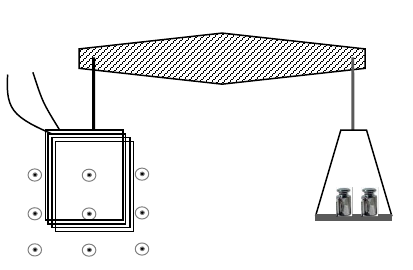
\includegraphics[scale=0.6]{m02.png}
  \captionof{figure}{Problema \ref{p:fmagnetica02}\label{f:fmagnetica02}}
\end{minipage}
%
\begin{Exercise}\label{p:fmagnetica03}
  La figura \ref{f:fmagnetica03} muestra una bobina con 20 espiras cuadradas, de lado igual $\SI{5}{\centi\metre}$, por la que circula la corriente $i = \SI{0.10}{\ampere}$. Verificar que el momento sobre una espira puede calcularse como $\va*{M} = \va*{m} \times \va*{B}$, donde $\va*{m}$ es el momento magnético de la espira, y hallar qué momento actúa sobre la bobina si está colocada de forma que el plano forma un ángulo $\alpha = \SI{60}{\degree}$ con respecto al eje $i$, en presencia de un campo magnético uniforme $\va*{B} = \SI{0.50}{\tesla}\vu{j}$.
\end{Exercise}
\begin{Answer}
  $\va*{M} = \SI{-2.17E-3}{\newton . \metre}\vu{k}$
\end{Answer}
%
\begin{Exercise}\label{p:fmagnetica04}
  Una barra conductora tiene $\SI{40}{\centi\metre}$ de longitud y $\SI{30}{\gram}$ de masa, y desliza libremente sobre las tiras metálicas de los extremos del plano inclinado mostrado en la figura \ref{f:fmagnetica04}, conectadas entre sí por un segmento conductor en la base de la rampa, mientras una corriente $i$ fluye a través del circuito indicado. El ángulo del plano inclinado es $\alpha = \SI{37}{\degree}$ y el sistema está inmerso en un campo magnético uniforme $\va*{B} = \SI{-0.20}{\tesla}\vu{y}$. ¿De qué magnitud debe ser $i$ para que la barra permanezca en reposo?
\end{Exercise}
\begin{Answer}
  $\SI{2.77}{\ampere}$
\end{Answer}
%
\noindent
\begin{minipage}[c]{0.5\textwidth}
  \begin{center}
    \tdplotsetmaincoords{70}{120}
    \begin{tikzpicture}[tdplot_main_coords, scale=0.7]
      \draw[axis] (0,0,0) -- (4,0,0) node [pos=1.1] {$i$};
      \draw[axis] (0,0,0) -- (0,4,0) node [pos=1.05] {$j$};
      \draw[axis] (0,0,0) -- (0,0,4)  node [left] {$k$};
      \draw[] (0,0,0) -- (2,3,0) -- (2,3,3) -- (0,0,3) -- cycle;
      \draw[] (0.1,-0.05,0) -- (2.1,2.95,0) -- (2.1,2.95,3) -- (0.1,-0.05,3) -- cycle;
      \draw[] (-0.1,0.05,0) -- (1.9,3.05,0) -- (1.9,3.05,3) -- (-0.1,0.05,3) -- cycle;
      \draw[red, -{latex}, very thick] (0.2,0,1) -- (0.2,0,2.5) node [midway, left] {$i$};
      \draw[red, -{latex}, thick] (0.9,-2.5,1.25) -- (0.9,-0.5,1.25);
      \draw[red, -{latex}, thick] (0.9,3,1.25) -- (0.9,5,1.25) node [midway, above] {$\va*{B}$};
      \draw[red, -{latex}, thick] (0.9,-2.5,2.5) -- (0.9,-0.5,2.5);
      \draw[red, -{latex}, thick] (0.9,3,2.5) -- (0.9,5,2.5);
      \draw[red, -{latex}, thick] (0.9,-2.5,0) -- (0.9,-0.5,0);
      \draw[red, -{latex}, thick] (0.9,3,0) -- (0.9,5,0);
      \draw[-latex] (0:2.5) arc (0:53:2.5) node[black,midway,below] {$\alpha$};
    \end{tikzpicture}
    \captionof{figure}{Problema \ref{p:fmagnetica03}\label{f:fmagnetica03}}
  \end{center}
\end{minipage}
%
\begin{minipage}[c]{0.5\textwidth}
\begin{center}
  \tdplotsetmaincoords{50}{110}
  \begin{tikzpicture}[tdplot_main_coords, scale=0.7]
    \draw[axis] (0,0,0) -- (4.5,0,0) node [pos=1.1] {$z$};
    \draw[axis] (0,0,0) -- (0,7,0) node [pos=1.05] {$x$};
    \draw[axis] (0,0,0) -- (0,0,3)  node [left] {$y$};
    \filldraw[draw=black,fill=black!50!green!50] (0,0,0) -- (0,6,3) -- (0.2,6,3) -- (0.2,0,0) -- cycle;
    \filldraw[draw=black, fill=black!50!green!50] (3,0,0) -- (3,6,3) -- (3.2,6,3) -- (3.2,0,0) -- cycle;
    \filldraw[draw=black, fill=black!50!green!50] (0,0,0) -- (3.2,0,0) -- (3.2,-0.2,0) -- (0,-0.2,0) -- cycle;
    \filldraw[draw=black, fill=red!30] (3.2,4,2) -- (3.2,4.402,2.201) -- (3.2,4.301, 2.402) -- (3.2, 3.9, 2.201) -- cycle;
    \filldraw[draw=black, fill=red!40] (3.2,3.9,2.201) -- (3.2,4.301,2.402) -- (0,4.301,2.403) -- (0,3.9,2.201) -- cycle;
    \filldraw[draw=black, fill=red!60] (3.2,4.301,2.402) -- (0,4.301,2.402) -- (0,4.402,2.201,2.402) -- (3.2,4.402,2.201,2.402) -- cycle;
    \draw[dotted] (3.1,0,0) -- (3.1,6,0);
    \draw[dotted] (0,6,0) -- (0,6,3) -- (3.1,6,3) -- (3.1,6,0) -- cycle;
    \draw[red, -{latex}, thick] (2.5,-0.3,0) -- (0.5,-0.3,0) node [midway, left] {$i$};
    \draw[red, -{latex}, thick] (-0.2,1,0.5) -- (-0.2,3,1.5) node [midway, above] {$i$};
    \draw[red, -{latex}, thick] (3.4,3,1.5) -- (3.4,1,0.5) node [midway, below] {$i$};
    \tdplotdrawarc{(3.1,1,0)}{2.5}{90}{136}{right}{$\alpha$}
  \end{tikzpicture}
  \captionof{figure}{Problema \ref{p:fmagnetica04}\label{f:fmagnetica04}}
\end{center}
\end{minipage}
%
\begin{Exercise}\label{p:fmagnetica05}
  Un conductor que transporta una corriente $i = \SI{3.0}{\ampere}$, está doblado sobre el plano $xy$ como se muestra en la figura \ref{f:fmagnetica05} y permanece en una zona donde existe un campo magnético $\va*{B} = \SI{0.70}{\tesla}\vu{x}$. El radio $R$ del semicírculo es $\SI{0.50}{\metre}$. ¿A qué fuerza está sometido el conductor?
\end{Exercise}
\begin{Answer}
  $\va*{F} = \SI{-2.1}{\newton}\vu{z}$
\end{Answer}
%
\begin{Exercise}\label{p:fmagnetica06}
  Mostrar que para la espira de la figura \ref{f:fmagnetica06}, por la cual circula una corriente y se encuentra sumergida en un campo magnético uniforme perpendicular al plano de la espira, la fuerza resultante es nula.
\end{Exercise}
%
\noindent
\begin{minipage}[c]{0.5\textwidth}
\begin{center}
  \begin{tikzpicture}[scale=0.5]
    \draw (5,0) ellipse (0.05 and 0.1);
    \draw [black] (0,0.1)--(5,0.1);
    \draw [black] (0,-0.1)--(5,-0.1);
    \draw [black] (0,0.1) arc (270:90:3);
    \draw [black] (0,-0.1) arc (270:90:3.2);
    \draw (5,6.2) ellipse (0.05 and 0.1);
    \draw [black] (0,6.1)--(5,6.1);
    \draw [black] (0,6.3)--(5,6.3);
    \draw [red, -{Stealth}, thick] (1,5.8)--(3,5.8) node[midway,below] {$i$};
    \draw [red, -{Stealth}, thick] (3,0.5)--(1,0.5) node[midway,above] {$i$};
    \draw [red, -{Stealth}, thick] (-1.84,1.26) arc (225:180:2.6) node[midway,right] {$i$};
    \draw [blue, -{Stealth}] (1,2)--(3,2) node[black,right,right] {$x$};
    \draw [blue, -{Stealth}] (1.3,1.7)--(1.3,3.7) node[black,above,left] {$y$};
    \draw [dotted] (0,0.1)--(0,6.1);
    \draw [dashed] (0,3.1)--(-2.12,5.22) node[midway,above] {$R$};
    \draw [blue, -{Stealth}] (-6,3.1)--(-4,3.1) node[pos=-0.2] {$\va*{B}$};
    \draw [blue, -{Stealth}] (-6,2.1)--(-4,2.1);
    \draw [blue, -{Stealth}] (-6,1.1)--(-4,1.1);
    \draw [blue, -{Stealth}] (-6,0.1)--(-4,0.1);
    \draw [blue, -{Stealth}] (-6,4.1)--(-4,4.1);
    \draw [blue, -{Stealth}] (-6,5.1)--(-4,5.1);
    \draw [blue, -{Stealth}] (-6,6.1)--(-4,6.1);
  \end{tikzpicture}
  \captionof{figure}{Problema \ref{p:fmagnetica05}\label{f:fmagnetica05}}
\end{center}
\end{minipage}
%
\begin{minipage}[c]{0.5\textwidth}
\begin{center}
  \begin{tikzpicture}[scale=0.5]
    \draw [very thick] (-2.21,0.79) arc (225:-45:3) -- (0,3) -- cycle;
    \draw [dotted] (-0.88,2.12) -- (0,1.5) -- (0.88,2.12);
    \draw (0,1.2) node [right] {$\SI{90}{\degree}$};
    \def\a{-4};
    \def\b{0.4};
    \def\d{2};
    \foreach \x in {0,...,4}
    \foreach \y [count=\yi] in {0,...,3}
    {
      \fill [blue!100!black!50] (\a+\d*\x,\b+\d*\y) circle (3pt);
      \draw [blue!100!black!50] (\a+\d*\x,\b+\d*\y) circle (7pt);
    }
  \end{tikzpicture}
  \captionof{figure}{Problema \ref{p:fmagnetica06}\label{f:fmagnetica06}}
\end{center}
\end{minipage}
%
\begin{Exercise}
  Un electrón se está moviendo con una velocidad de $\SI{4E6}{\metre/\second}$ en la dirección positiva del eje $x$, cuando ingresa en una zona del espacio donde existe un campo eléctrico uniforme $\va*{E} = \SI{2000}{\volt/\metre}\vu{y}$. Encontrar el campo magnético necesario para que en esa región el electrón no se desvíe de su trayectoria.
\end{Exercise}
\begin{Answer}
  $\va*{B} = \SI{5E-4}{\tesla}\vu{z}$
\end{Answer}
%
\begin{Exercise}\label{p:fmagnetica07}
  Un electrón pasa por el punto $A$ de la figura \ref{f:fmagnetica07} con una velocidad de módulo $V_0 = \SI{1E7}{\metre/\second}$. Calcular: \textit{a}) El valor y el sentido del campo magnético uniforme que obliga al electrón a seguir la trayectoria semicircular desde $A$ hacia $B$. \textit{b}) El tiempo necesario para que el electrón se mueva desde $A$ hasta $B$.
\end{Exercise}
\begin{Answer}
  \begin{minipage}[t]{.4\textwidth}
    \textit{a}) $\SI{1.138E-3}{\tesla}$, perpendicular y entrando a la hoja\\ \textit{b}) $\SI{1.57E-8}{\second}$
  \end{minipage}
\end{Answer}
%
\begin{Exercise}\label{p:fmagnetica08}
  Un ion que parte del reposo en el vacío es acelerado por dos placas paralelas entre las que existe una ddp de $\SI{1000}{\volt}$ como indica la figura \ref{f:fmagnetica08}. Al salir de la segunda placa, el ion se mueve bajo la acción de un campo magnético uniforme de módulo $B = \SI{0.1}{\tesla}$, normal al plano de la trayectoria. Si el radio de curvatura de la trayectoria es $\SI{0.3}{\metre}$, ¿cuál es la masa del ion si su carga es la del electrón?
\end{Exercise}
\begin{Answer}
  $\SI{7.2E-26}{\kilogram}$
\end{Answer}
%
\noindent
\begin{minipage}[c]{0.5\textwidth}
\begin{center}
  \begin{tikzpicture}[scale=0.5]
    \draw [blue, -{Stealth}] (0,0) -- (0,3) node [left] {$V_0$};
    \draw [dashed] (0,0) arc (180:0:5);
    \draw [dotted] (0,0) -- (10,0);
    \draw [{Stealth}-{Stealth}] (0,-0.5) -- (10,-0.5) node[midway,below] {$\SI{10}{\centi\metre}$};
    \draw [] (0,-0.3) -- (0,-0.8);
    \draw [] (10,-0.3) -- (10,-0.8);
    \draw (0,0) node [left] {$A$};
    \draw (10,0) node [right] {$B$};
  \end{tikzpicture}
  \captionof{figure}{Problema \ref{p:fmagnetica07}\label{f:fmagnetica07}}
\end{center}
\end{minipage}
%
\begin{minipage}[c]{0.5\textwidth}
\begin{center}
  \begin{tikzpicture}[scale=0.5]
    \draw [] (-7,3.4) -- (-4,3.4) arc (90:0:5) ;
    \draw [blue!100!black!60] (-1.9,4.4) node[above right] {$\va*{B}$};
    \filldraw [draw=black, fill=black!30] (-5,0.4) -- (-5,3.2) -- (-4.7,3.2) -- (-4.7,0.4) -- cycle;
    \filldraw [draw=black, fill=black!30] (-5,3.6) -- (-5,6.4) -- (-4.7,6.4) -- (-4.7,3.6) -- cycle;
    \filldraw [draw=black, fill=black!30] (-5.9,0.4) -- (-5.9,3.2) -- (-5.6,3.2) -- (-5.6,0.4) -- cycle;
    \filldraw [draw=black, fill=black!30] (-5.9,3.6) -- (-5.9,6.4) -- (-5.6,6.4) -- (-5.6,3.6) -- cycle;
    \def\a{-4};
    \def\b{0.4};
    \def\d{2};
    \foreach \x in {0,...,4}
    \foreach \y [count=\yi] in {0,...,3}
    {
      % \fill [blue!100!black!50] (\a+\d*\x,\b+\d*\y) circle (3pt);
      \draw [blue!100!black!50] (\a+\d*\x-0.2828,\b+\d*\y-0.2828) -- (\a+\d*\x+0.2828,\b+\d*\y+0.2828);
      \draw [blue!100!black!50] (\a+\d*\x+0.2828,\b+\d*\y-0.2828) -- (\a+\d*\x-0.2828,\b+\d*\y+0.2828);
      \draw [blue!100!black!50] (\a+\d*\x,\b+\d*\y) circle (0.4);
    }
  \end{tikzpicture}
  \captionof{figure}{Problema \ref{p:fmagnetica08}\label{f:fmagnetica08}}
\end{center}
\end{minipage}
%
\begin{Exercise}
  Un electrón con una energía de $\SI{2.0}{keV}$ se dispara en un campo uniforme de $\SI{0.10}{\tesla}$ y su velocidad forma un ángulo de $\SI{89}{\degree}$ con el mismo. Muestre que la trayectoria será una hélice, con su eje en la dirección del campo. Encuentre el periodo $T$, el paso $p$ y el radio $r$ de la hélice.
\end{Exercise}
\begin{Answer}
  \begin{minipage}[t]{.4\textwidth}
    $T=\SI{3.57E-10}{\second}$\\ $p=\SI{0.16}{\milli\metre}$\\ $r=\SI{1.5}{\milli\metre}$
  \end{minipage}
\end{Answer}


  % \colorsection{Ley de Biot-Savart y Ley de Amp\`ere}
\setcounter{figure}{0}

\begin{Exercise}\label{p:magnetico01}
    Calcular el módulo del campo magnético en el punto $P$, ubicado en el punto medio entre los dos cables paralelos mostrados en la figura \ref{f:magnetico01}. Los cables pueden considerarse rectos e infinitos.
\end{Exercise}
\begin{Answer}
    $\SI{5E-6}{\tesla}$
\end{Answer}
%
\begin{Exercise}\label{p:magnetico02}
    La figura \ref{f:magnetico02} muestra las corrientes transportadas por tres cables infinitos y paralelos al eje $x$. \textit{a}) Determinar el vector campo magnético resultante en el punto $P$, ubicado sobre el eje $z$ a $\SI{3}{\centi\metre}$ arriba del cable central. \textit{b}) Calcular la fuerza neta por unidad de longitud ejercida sobre el cable central.
\end{Exercise}
\begin{Answer}
    \begin{minipage}[t]{.4\textwidth}
        \textit{a}) $\va*{B} = (1.03\vu{y}-1.12\vu{z})\SI{E-4}{\tesla}$\\ \textit{b}) $\va*{F}/l = \SI{4.55E-3}{\newton/\metre}\vu{y}$
    \end{minipage}
\end{Answer}
%
\noindent
\begin{minipage}[c]{0.5\textwidth}
\begin{center}
    \begin{tikzpicture}[scale=0.5]
        \draw (6,0) ellipse (0.1 and 0.2);
        \draw (-5,0) +(90:0.1 and 0.2) arc (90:270:0.1 and 0.2);
        \draw [black] (-5,0.2)--(6,0.2);
        \draw [black] (-5,-0.2)--(6,-0.2);
        \draw [red, -{Stealth}, thick] (-4,0)--(-1,0) node[midway,above] {$\SI{1}{\ampere}$};
        \draw (6,3) ellipse (0.1 and 0.2);
        \draw (-5,3) +(90:0.1 and 0.2) arc (90:270:0.1 and 0.2);
        \draw [black] (-5,3.2)--(6,3.2);
        \draw [black] (-5,2.8)--(6,2.8);
        \draw [red, -{Stealth}, thick] (-4,3)--(-1,3) node[midway,above] {$\SI{2}{\ampere}$};
        \fill [blue] (0,1.5) circle (0.15) node[right] {$P$};
        \draw [{Stealth}-{Stealth}] (-5.5,0) -- (-5.5,3) node[midway, left] {$\SI{8}{\centi\metre}$};
    \end{tikzpicture}
    \captionof{figure}{Problema \ref{p:magnetico01}\label{f:magnetico01}}
\end{center}
\end{minipage}
%
\begin{minipage}[c]{0.5\textwidth}
\begin{center}
    \def\alfa{70}
    \def\beta{110}
    \def\radio{0.15}
    \def\d{2}
    \tdplotsetmaincoords{\alfa}{\beta}
    \begin{tikzpicture}[tdplot_main_coords, scale=0.7]
        \draw[axis] (6,0,0) -- (10,0,0) node [pos=1.1] {$x$};
        \draw[blue, dotted] (6,0,0) -- (-4,0,0);
        \draw[blue, dotted] (0,0,0) -- (0,\radio,0);

        \draw[blue, thick] (0,-\d,0) -- (0,-\d-2,0);
        \fill [white] (6,{-\d-\radio*cos(-2*\alfa)},{\radio*sin(-2*\alfa)}) -- (-4,{-\d-\radio*cos(-2*\alfa)},{\radio*sin(-2*\alfa)}) -- (-4,{-\d+\radio*cos(-2*\alfa)},{-\radio*sin(-2*\alfa)}) -- (6,{-\d+\radio*cos(-2*\alfa)},{-\radio*sin(-2*\alfa)}) -- cycle;
        \draw[blue, thick] (0,\radio,0) -- (0,-\d+\radio,0);
        \fill [white] (6,{-\radio*cos(-2*\alfa)},{\radio*sin(-2*\alfa)}) -- (-4,{-\radio*cos(-2*\alfa)},{\radio*sin(-2*\alfa)}) -- (-4,{\radio*cos(-2*\alfa)},{-\radio*sin(-2*\alfa)}) -- (6,{\radio*cos(-2*\alfa)},{-\radio*sin(-2*\alfa)}) -- cycle;
        \draw[blue, thick] (0,\radio,0) -- (0,\d,0);

        \draw[axis] (0,0,\radio) -- (0,0,4)  node [left] {$z$};
        \draw[blue, dotted] (0,0,0) -- (0,0,\radio);
        \fill [white] (6,{\d+-\radio*cos(-2*\alfa)},{\radio*sin(-2*\alfa)}) -- (-4,{\d+-\radio*cos(-2*\alfa)},{\radio*sin(-2*\alfa)}) -- (-4,{\d+\radio*cos(-2*\alfa)},{-\radio*sin(-2*\alfa)}) -- (6,{\d+\radio*cos(-2*\alfa)},{-\radio*sin(-2*\alfa)}) -- cycle;
        \draw[axis] (0,\d+\radio,0) -- (0,4,0) node [pos=1.05] {$y$};

        \draw [] (6,{-\radio*cos(-2*\alfa)},{\radio*sin(-2*\alfa)}) -- (-4,{-\radio*cos(-2*\alfa)},{\radio*sin(-2*\alfa)});
        \draw [] (6,{\radio*cos(-2*\alfa)},{-\radio*sin(-2*\alfa)}) -- (-4,{\radio*cos(-2*\alfa)},{-\radio*sin(-2*\alfa)});
        \draw[] plot[domain=0:6.2831853,smooth,variable=\t] (6, {\radio*cos(\t r)},{\radio*sin(\t r)});

        \draw [] (6,{\d+-\radio*cos(-2*\alfa)},{\radio*sin(-2*\alfa)}) -- (-4,{\d+-\radio*cos(-2*\alfa)},{\radio*sin(-2*\alfa)});
        \draw [] (6,{\d+\radio*cos(-2*\alfa)},{-\radio*sin(-2*\alfa)}) -- (-4,{\d+\radio*cos(-2*\alfa)},{-\radio*sin(-2*\alfa)});
        \draw[] plot[domain=0:6.2831853,smooth,variable=\t] (6, {\d+\radio*cos(\t r)},{\radio*sin(\t r)});

        \draw [] (6,{-\d+-\radio*cos(-2*\alfa)},{\radio*sin(-2*\alfa)}) -- (-4,{-\d+-\radio*cos(-2*\alfa)},{\radio*sin(-2*\alfa)});
        \draw [] (6,{-\d+\radio*cos(-2*\alfa)},{-\radio*sin(-2*\alfa)}) -- (-4,{-\d+\radio*cos(-2*\alfa)},{-\radio*sin(-2*\alfa)});
        \draw[] plot[domain=0:6.2831853,smooth,variable=\t] (6, {-\d+\radio*cos(\t r)},{\radio*sin(\t r)});

        \draw[dotted] (6,-\d,0) -- (8,-\d,0);
        \draw[dotted] (6,\d,0) -- (8,\d,0);
        \draw [{Stealth[slant={0.5}]}-{Stealth[slant={0.5}]}] (7.5,-\d,0) -- (7.5,0,0) node [midway,below, sloped, xslant=0.5] {$\SI{4}{\centi\metre}$};
        \draw [{Stealth[slant={0.5}]}-{Stealth[slant={0.5}]}] (7.5,\d,0) -- (7.5,0,0) node [midway,below, sloped, xslant=0.5] {$\SI{4}{\centi\metre}$};

        \draw [red, -{Stealth}, thick] (1,-\d, 0) -- (-2,-\d,0) node[midway,above, sloped, xslant=0.5] {$\SI{75}{\ampere}$};
        \draw [red, -{Stealth}, thick] (1,\d, 0) -- (-2,\d,0) node[midway,above, sloped, xslant=0.5] {$\SI{40}{\ampere}$};
        \draw [red, -{Stealth}, thick] (2,0,0) -- (5,0,0) node[midway,above, sloped, xslant=0.5] {$\SI{26}{\ampere}$};

        \fill [red] (0,0,2) circle (0.15) node [above right] {$P$};

    \end{tikzpicture}
    \captionof{figure}{Problema \ref{p:magnetico02}\label{f:magnetico02}}
\end{center}
\end{minipage}
%
\begin{Exercise}\label{p:magnetico03}
    La figura \ref{f:magnetico03} muestra tres cables infinitos, paralelos entre sí, que pasan perpendicularmente a la página por los vértices del triángulo mostrado. Las corrientes $i_1$ e $i_3$ salen de la página y valen $\SI{20}{\ampere}$ y $\SI{32}{\ampere}$ respectivamente, y la corriente $i_2$ entra a la página y vale $\SI{20}{\ampere}$. Calcular el módulo de la fuerza neta por unidad de longitud que las corrientes $i_1$ e $i_2$ ejercen sobre el conductor que transporta a $i_3$.
\end{Exercise}
\begin{Answer}
    $\SI{3.0E-3}{\newton/\metre}$
\end{Answer}
%
\begin{Exercise}\label{p:magnetico04}
    Calcular el módulo del campo magnético producido por la corriente $i = \SI{15}{\ampere}$ que circula por un segmento de cable de longitud $L = \SI{0.20}{\metre}$, en el punto $P$ ubicado a una distancia $L/2$ del centro del cable, como se muestra en la figura \ref{f:magnetico04}.
\end{Exercise}
\begin{Answer}
    $\SI{2.12E-5}{\tesla}$
\end{Answer}
%
\noindent
\begin{minipage}[c]{0.5\textwidth}
\begin{center}
    \begin{tikzpicture}[scale=0.5]
      \draw [blue!100!black!50] (5-0.2828,-0.2828) -- (5+0.2828,0.2828);
      \draw [blue!100!black!50] (5+0.2828,-0.2828) -- (5-0.2828,0.2828);
      \draw [blue!100!black!50] (5,0) circle (0.4);
      \fill [blue!100!black!50] (0,0) circle (0.2);
      \draw [blue!100!black!50] (0,0) circle (0.4);
      \fill [blue!100!black!50] (0,5) circle (0.2);
      \draw [blue!100!black!50] (0,5) circle (0.4);
      \draw [dotted] (0,0) -- (5,0) -- (0,5) -- (0,0);
      \draw [] (-.8,0) node [] {$i_1$};
      \draw [] (-.8,5) node [] {$i_3$};
      \draw [] (5.8,0) node [] {$i_2$};
      \draw [] (-1.5,5) -- (-2.5,5);
      \draw [] (-1.5,0) -- (-2.5,0);
      \draw [{Stealth}-{Stealth}] (-2.2,0) -- (-2.2,5) node [midway,left] {$\SI{3}{\centi\metre}$};
      \draw [] (0,-1) -- (0,-2);
      \draw [] (5,-1) -- (5,-2);
      \draw [{Stealth}-{Stealth}] (0,-1.7) -- (5,-1.7) node [midway,below] {$\SI{3}{\centi\metre}$};
    \end{tikzpicture}
    \captionof{figure}{Problema \ref{p:magnetico03}\label{f:magnetico03}}
\end{center}
\end{minipage}
%
\begin{minipage}[c]{0.5\textwidth}
\begin{center}
    \begin{tikzpicture}[scale=0.5]
        \draw (5,0) ellipse (0.1 and 0.2);
        \draw (-5,0) +(90:0.1 and 0.2) arc (90:270:0.1 and 0.2);
        \draw [black] (-5,0.2)--(5,0.2);
        \draw [black] (-5,-0.2)--(5,-0.2);
        \draw [red, -{Stealth}, thick] (-4,0)--(-1,0) node[midway,above] {$i$};
        \fill [blue] (0,5) circle (0.15) node[right] {$P$};
        \draw [{Stealth}-{Stealth}] (0,0.3) -- (0,4.7) node[midway, right] {$L/2$};
        \draw [{Stealth}-{Stealth}] (-5,-0.8) -- (5,-0.8) node[midway, below] {$L$};
    \end{tikzpicture}
    \captionof{figure}{Problema \ref{p:magnetico04}\label{f:magnetico04}}
\end{center}
\end{minipage}
%
\begin{Exercise}
    Determinar el módulo del campo magnético en el centro de una espira cuadrada de $\SI{4}{\centi\metre}$ de lado, que transporta una corriente de $\SI{28}{\ampere}$.
\end{Exercise}
\begin{Answer}
    $\SI{7.92E-4}{\tesla}$
\end{Answer}
%
\begin{Exercise}\label{p:magnetico05}
    Un alambre recto que transporta una corriente $i_1$ está colocado sobre el eje de una espira circular por la que corre una corriente $i_2$, como se muestra en la figura \ref{f:magnetico05}. Demostrar que la fuerza ejercida por la espira sobre el alambre es nula.
\end{Exercise}
%
\begin{Exercise}\label{p:magnetico06}
    Un hilo muy largo tiene un bucle semicircular de radio $R$ como indica la figura \ref{f:magnetico06}. Si por el hilo circula una corriente $i$, verificar que el campo magnético en el centro $P$ es:
    \begin{align*}
        B &= \dfrac{\mu_0 i}{4R} \quad \text{entrando a la página}
    \end{align*}
\end{Exercise}
%
\begin{Exercise}\label{p:magnetico07}
    Calcular el campo magnético (módulo y sentido) en el punto $P$ producido por la corriente que circula en el conductor mostrado en la figura \ref{f:magnetico07}. Datos: $i = \SI{20}{\ampere}$; $a = \SI{5}{\centi\metre}$; $b = \SI{10}{\centi\metre}$.
\end{Exercise}
\begin{Answer}
    \begin{minipage}[c]{0.4\textwidth}
        $\SI{6.28E-5}{\tesla}$, saliendo de la página.
    \end{minipage}
\end{Answer}
%
\noindent
\begin{minipage}[c]{0.5\textwidth}
\begin{center}
    \def\alfa{70}
    \def\beta{140}
    \def\radio{0.15}
    \def\radiob{2.2}
    \def\d{0.3}
    \tdplotsetmaincoords{\alfa}{\beta}
    \begin{tikzpicture}[tdplot_main_coords, scale=0.6]
        \draw[] plot[domain=0:6.2831853,smooth,variable=\t] (0, {\radiob*cos(\t r)},{\radiob*sin(\t r)});
        \draw[] plot[domain=0:6.2831853,smooth,variable=\t] (0, {(\radiob+\d)*cos(\t r)},{(\radiob+\d)*sin(\t r)});
        \draw[red, -{Stealth[reversed]}, thick] plot[domain=0.3:1.2,smooth,variable=\t] (0, {(\radiob+\d/2)*cos(\t r)},{(\radiob+\d/2)*sin(\t r)});
        \draw (0,{(\radiob+\d+0.5)*0.71},{(\radiob+\d+0.5)*0.71}) node [red] {$i_2$};

        \fill [white] (6,{-\radio*cos(-2*\alfa)},{\radio*sin(-2*\alfa)}) -- (-1,{-\radio*cos(-2*\alfa)},{\radio*sin(-2*\alfa)}) -- (-1,{\radio*cos(-2*\alfa)},{-\radio*sin(-2*\alfa)}) -- (6,{\radio*cos(-2*\alfa)},{-\radio*sin(-2*\alfa)}) -- cycle;

        \draw [] (6,{-\radio*cos(-2*\alfa)},{\radio*sin(-2*\alfa)}) -- (-1,{-\radio*cos(-2*\alfa)},{\radio*sin(-2*\alfa)});
        \draw [] (6,{\radio*cos(-2*\alfa)},{-\radio*sin(-2*\alfa)}) -- (-1,{\radio*cos(-2*\alfa)},{-\radio*sin(-2*\alfa)});
        \draw[] plot[domain=0:6.2831853,smooth,variable=\t] (6, {\radio*cos(\t r)},{\radio*sin(\t r)});
        \draw [] (-2,{-\radio*cos(-2*\alfa)},{\radio*sin(-2*\alfa)}) -- (-5,{-\radio*cos(-2*\alfa)},{\radio*sin(-2*\alfa)});
        \draw [] (-2,{\radio*cos(-2*\alfa)},{-\radio*sin(-2*\alfa)}) -- (-5,{\radio*cos(-2*\alfa)},{-\radio*sin(-2*\alfa)});

        \draw [red, -{Stealth}, thick] (5,0,0) -- (2,0,0) node[midway,above] {$i_1$};
    \end{tikzpicture}
    \captionof{figure}{Problema \ref{p:magnetico05}\label{f:magnetico05}}
\end{center}
\end{minipage}
%
\begin{minipage}[c]{0.5\textwidth}
    \begin{center}
        \begin{tikzpicture}[scale=0.6]
            \draw (7,0) ellipse (0.1 and 0.2);
            \draw (4.2,-0.2) arc (0:180:4);
            \fill [white] (4.3,0.2) -- (-4.3,0.2) -- (-4.3,-0.2) -- (4.3,-0.2) -- cycle;
            \draw (7,-0.2) -- (3.8,-0.2) arc (0:180:3.6) -- (-7,-0.2);
            \draw [black] (-7,0.2)--(-3.8,0.2);
            \draw [black] (7,0.2)--(4.2,0.2);
            \draw (-7,0) +(90:0.1 and 0.2) arc (90:270:0.1 and 0.2);
            \draw [red, -{Stealth}, thick] (-6,0)--(-4,0) node[midway,above] {$i$};
            \fill [blue] (0,0) circle (0.15) node[left] {$P$};
            \draw [-{Stealth}] (0,0) -- (3.6*0.71,3.6*0.71) node[midway, above left] {$R$};
        \end{tikzpicture}
        \captionof{figure}{Problema \ref{p:magnetico06}\label{f:magnetico06}}
    \end{center}
\end{minipage}
%
\noindent
\begin{minipage}[c]{0.5\textwidth}
    \begin{center}
        \begin{tikzpicture}[scale=0.6]
            % \draw (7,0) ellipse (0.1 and 0.2);
            \draw (5.6,-0.2) arc (0:180:5.6);
            \draw (2.5,-0.2) arc (0:180:2.5);
            \fill [white] (6,0.2) -- (-6,0.2) -- (-6,-0.2) -- (6,-0.2) -- cycle;
            \draw (2.1,-0.2) arc (0:180:2.1);
            \draw (6,-0.2) arc (0:180:6);
            \draw [black] (5.6,0.2)--(2.5,0.2);
            \draw [black] (-5.6,0.2)--(-2.5,0.2);
            \draw [black] (6,-0.2)--(2.1,-0.2);
            \draw [black] (-6,-0.2)--(-2.1,-0.2);
            \draw [red, -{Stealth}, thick] (-3,0)--(-5,0) node[midway,above] {$i$};
            \draw [red, -{Stealth}, thick] (5,0)--(3,0);
            \draw [red, -{Stealth}, thick] (-5.8*0.71,-0.2+5.8*0.71) arc (135:110:5.8);
            \draw [red, -{Stealth}, thick] (0,-0.2+2.3) arc (90:135:2.3);
            \fill [blue] (0,0) circle (0.15) node[left] {$P$};
            \draw [-{Stealth}] (0,0) -- (2.3*0.866,2.3*0.5) node[pos=0.5, below] {$a$};
            \draw [-{Stealth}] (0,0) -- (5.8*0.71,5.8*0.71) node[pos=0.5, above] {$b$};
        \end{tikzpicture}
        \captionof{figure}{Problema \ref{p:magnetico07}\label{f:magnetico07}}
    \end{center}
\end{minipage}
%
\begin{minipage}[c]{0.5\textwidth}
    \begin{center}
        \begin{tikzpicture}[scale=0.6]
            \draw (7,0) ellipse (0.1 and 0.2);
            \draw (7,7.6) ellipse (0.1 and 0.2);
            \draw (7,-0.2) -- (0,-0.2) arc (270:90:4) -- (7,7.8);
            \draw (7,0.2) -- (0,0.2) arc (270:90:3.6) -- (7,7.4);
            \fill [blue] (0,4) circle (0.15) node[below left] {$P$};
            \draw [-{Stealth}] (0,4) -- (-3.7*0.71,4+3.7*0.71) node[midway, right] {$R$};
            \draw[axis] (3,4) -- (6,4) node [pos=1.1] {$x$};
            \draw[axis] (3.4,3.6) -- (3.4,6.6) node [left] {$y$};
            \draw [red, -{Stealth}, thick] (6,7.6)--(3,7.6) node[midway,above] {$i$};
            \draw [red, -{Stealth}, thick] (3,0)--(6,0) node[midway,above] {$i$};
            \draw [red, -{Stealth}, thick] (-3.8,3.8) arc (180:210:3.8);
        \end{tikzpicture}
        \captionof{figure}{Problema \ref{p:magnetico08}\label{f:magnetico08}}
    \end{center}
\end{minipage}
%
\begin{Exercise}\label{p:magnetico08}
    Un hilo largo que transporta una corriente $i$ se curva en forma de horquilla como muestra la figura \ref{f:magnetico08}. Demostrar que el campo magnético en $P$, situado en el centro de la semicircunferencia, vale:
    \begin{align*}
        \va*{B} &= \dfrac{\mu_0 i}{2R} \left ( \dfrac{1}{2} + \dfrac{1}{\pi} \right ) \vu{z}
    \end{align*}
\end{Exercise}
%
\noindent
\begin{minipage}[c]{0.5\textwidth}
\begin{Exercise}\label{p:magnetico09}
    Dos conductores coplanares se disponen como indica la figura \ref{f:magnetico09}. Considere a los conductores lineales e infinitos. Obtener la siguiente expresión para el módulo de la fuerza que ejercida sobre el segmento de longitud $b$ del conductor que transporta a $i_2$ como consecuencia del campo generado por la corriente $i_1$:
    \begin{align*}
        F &= \dfrac{\mu_0 i_1 i_2}{2\pi \sin\alpha} \ln \left ( \dfrac{a+b}{a}\right )
    \end{align*}
\end{Exercise}
\end{minipage}
%
\begin{minipage}[c]{0.5\textwidth}
    \begin{center}
        \def\alfa{45}
        \def\dx{3}
        \def\dy{0}
        \begin{tikzpicture}[scale=0.5]
            \draw (0,7) ellipse (0.2 and 0.1);
            \draw [] (-0.2,7) -- (-.2,0.5);
            \draw [] (0.2,7) -- (.2,0.5);

            \draw [cm={cos(\alfa) ,-sin(\alfa) ,sin(\alfa) ,cos(\alfa) ,(\dx,\dy)}] (0,8) ellipse (0.2 and 0.1);
            \draw [cm={cos(\alfa) ,-sin(\alfa) ,sin(\alfa) ,cos(\alfa) ,(\dx,\dy)}] (-0.2,8) -- (-.2,0);
            \draw [cm={cos(\alfa) ,-sin(\alfa) ,sin(\alfa) ,cos(\alfa) ,(\dx,\dy)}] (0.2,8) -- (.2,0);

            \draw [dotted] (0,0) -- (0,-3.5);
            \draw [dotted, cm={cos(\alfa) ,-sin(\alfa) ,sin(\alfa) ,cos(\alfa) ,(\dx,\dy)}] (0,-0.4) -- (0,-5);
            \draw (0,-2) arc (90:45:1) node [midway, above] {$\alpha$};
            \draw [red, -{Stealth}, thick] (0,6)--(0,4) node[midway,left] {$i_1$};
            \draw [red, -{Stealth}, thick,cm={cos(\alfa) ,-sin(\alfa) ,sin(\alfa) ,cos(\alfa) ,(\dx,\dy)} ] (0,5)--(0,7) node[midway,above left] {$i_2$};

            \fill [blue, fill opacity=0.4, cm={cos(\alfa) ,-sin(\alfa) ,sin(\alfa) ,cos(\alfa) ,(\dx,\dy)}] (-0.2,1.5) -- (-0.2,3.5) -- (0.2, 3.5) -- (0.2, 1.5) -- cycle;
            \draw [|-|, cm={cos(\alfa) ,-sin(\alfa) ,sin(\alfa) ,cos(\alfa) ,(\dx,\dy)}] (0.8,1.5) -- (0.8,-4.2) node [pos=0.4, below] {$a$};
            \draw [|-|, cm={cos(\alfa) ,-sin(\alfa) ,sin(\alfa) ,cos(\alfa) ,(\dx,\dy)}] (0.8,1.5) -- (0.8,3.5) node [pos=0.6, below] {$b$};
        \end{tikzpicture}
        \captionof{figure}{Problema \ref{p:magnetico09}\label{f:magnetico09}}
    \end{center}
\end{minipage}
%



  % \colorsection{Preguntas sobre campos para el análisis}
\textit{En esta sección se requiere brindar respuestas argumentadas.}
\setcounter{figure}{0}
%
\begin{Exercise}
    Imagine que tiene dos esferas metálicas ligeras y que cada una de ellas cuelga de un cordón de nailon aislante. Una de las esferas tiene carga neta negativa; en tanto que la otra no tiene carga neta. Si las esferas están cerca una de otra, pero no se tocan, ¿se atraerán mutuamente, se repelerán o no ejercerán fuerza alguna sobre la otra?
\end{Exercise}
%
\begin{Exercise}
Dado el caso anterior: ahora se permite que las esferas entren en contacto. Una vez que se tocan, ¿se atraerán, se repelerán o no ejercerán fuerza alguna sobre la otra?
\end{Exercise}
%
\begin{Exercise}
    Cuando una varilla de vidrio cargada se acerca a un trozo de papel descargado, el papel se siente atraído por la varilla. Explique porqué sucede esto aunque el papel sea un material no conductor y esté descargado.
\end{Exercise}
%
\begin{Exercise}
    Suponga que una carga puntual se encuentra fija en su posición. Entonces, si una partícula pequeña cargada positivamente se coloca en algún punto cercano a la carga fija y se libera, ¿la trayectoria de esta segunda partícula seguirá una línea de campo eléctrico? ¿Por qué?
\end{Exercise}
%
\begin{Exercise}
    Se coloca un protón en un campo eléctrico uniforme y luego se libera. Después se sitúa un electrón en el mismo punto y también se libera. ¿Las dos partículas experimentan la misma fuerza? ¿La misma aceleración? ¿Se mueven en la misma dirección cuando se liberan?
\end{Exercise}
%
\begin{Exercise}
    El potencial (en relación con un punto en el infinito) a media distancia entre dos cargas puntuales de igual magnitud y signos opuestos es igual a cero. Si se trae una carga de prueba desde el infinito hasta ese punto medio, el trabajo neto que es necesario entregar a esa carga, ¿es positivo, negativo o cero? ¿Es posible traer una carga de prueba desde el infinito hasta ese punto medio en forma tal que no se efectúe trabajo en ninguna parte del desplazamiento? Si es así, describa cómo se puede lograr. Si no es posible, explique por qué.
\end{Exercise}
%
\begin{Exercise}
    Es posible tener una configuración de dos cargas puntuales separadas por una distancia finita de manera que la energía potencial eléctrica del arreglo sea la misma que la de las dos cargas separadas por una distancia infinita? ¿Por qué? ¿Y si fueran tres cargas? Explique su razonamiento.
\end{Exercise}
%
\begin{Exercise}
    Como el potencial puede tener cualquier valor que se desee dependiendo de la elección del nivel de referencia de potencial cero, ¿cómo “sabe” un voltímetro qué lectura hacer cuando se conecta entre dos puntos?
\end{Exercise}
%
\begin{Exercise}
    Si se resuelve la integral del campo eléctricostático para una trayectoria cerrada, el resultado siempre será igual a cero, independientemente de la forma de la trayectoria y de dónde se localicen las cargas en relación con esta. Explique por qué es así.
\end{Exercise}
%
\begin{Exercise}
    La diferencia de potencial entre dos terminales de una batería AA (de las que se usan en las linternas) es de $\SI{1.5}{\volt}$. Si se colocan dos baterías AA extremo con extremo, con la terminal positiva de una batería en contacto con la terminal negativa de la otra, ¿cuál es la diferencia de potencial entre las terminales en los extremos expuestos de la combinación? ¿Qué pasa si las dos terminales positivas se tocan entre sí? Explique su razonamiento.
\end{Exercise}
%
\begin{Exercise}
    Es frecuente que se diga que si un punto $A$ tiene un potencial más elevado que un punto $B$, entonces $A$ tiene un potencial positivo y $B$ un potencial negativo. ¿Se concluye que un punto con potencial positivo está cargado positivamente, o que un punto con potencial negativo está cargado negativamente? Ilustre sus respuestas con ejemplos claros y sencillos.
\end{Exercise}
%

  \begin{titlepage}
    % \begin{figure}[ht]
    \begin{center}
    \vspace{1.5cm}
    % Aquí se inserta el escudo o emblema:
    \begin{tikzpicture}[scale=1, every node/.style={scale=1}]
    \definecolor{topcolor}{RGB}{0,121,138};
    \definecolor{botcolor}{RGB}{0,121,138};

    \fill[color=topcolor] (1.8273,1.065) arc (30.235:149.765:2.115) -- cycle;
    \fill[color=botcolor] (1.8273,-1.065) arc (-30.235:-149.765:2.115) -- cycle;

    \draw[color=botcolor, thick] (-1.755,-0.625) -- (1.755, -0.625);
    \fill[color=botcolor] (-1.755,-0.0929) -- (1.755, -0.0929) -- (1.755, -0.5405) -- (-1.755,-0.5405) -- cycle;

    % \fill [black](0,-0.7) circle(2pt);

    % \draw (-1.7539,0.93) rectangle (-0.9592,0);
    \fill[] (-1.7539,0.93) arc (180:360:0.39735) -- (-1.1178,0.93) arc (360:180:0.23875) -- cycle;
    \fill[] (-1.7539,0) arc (180:0:0.39735) -- (-1.1178,0) arc (0:180:0.23875) -- cycle;
    \fill (-1.7539,0.3866) rectangle (-0.9592,0.5434);
    \fill (-1.43495,0.93) rectangle (-1.27815,0);

    \fill[color=topcolor] (-0.7795,0.3275) arc[start angle=180, end angle=360,x radius=0.40585, y radius=0.3275] -- (0.0322,0.8506) arc[start angle=0, end angle=180,x radius=0.08925, y radius=0.0794] -- (-0.1463,0.3275) arc[start angle=0, end angle=-180,x radius=0.22735, y radius=0.1604] -- (-0.603, 0.8506) arc[start angle=0, end angle=180,x radius=0.08925, y radius=0.0794] -- cycle;

    \fill[color=topcolor] (0.4003,0.0794) arc[start angle=180, end angle=360,x radius=0.08925, y radius=0.0794] -- (0.5788,0.7515) -- (0.7986,0.7515) arc[start angle=-90, end angle=90,x radius=0.0794, y radius=0.08925] -- (0.1805,0.93) arc[start angle=90, end angle=270,x radius=0.0794, y radius=0.08925] -- (0.4003, 0.7515) -- cycle;

    \fill[color=topcolor] (0.9455,0.0794) arc[start angle=180, end angle=360,x radius=0.08925, y radius=0.0794] -- (1.124,0.608) -- (1.57,0.0267) arc[start angle=-153.217, end angle=0,x radius=0.09411, y radius=0.07059] -- (1.755,0.8506) arc[start angle=0, end angle=180,x radius=0.08925, y radius=0.0794] -- (1.5765,0.3191) -- (1.124,0.9004) arc[start angle=26.783, end angle=180,x radius=0.09411, y radius=0.07059] -- cycle;

    \node [scale=0.8,color=white] at (-1.3822,-0.31) {{\fontfamily{cmss}\selectfont \textbf{A}}};
    \node [scale=0.8,color=white] at (-1.0751,-0.31) {{\fontfamily{cmss}\selectfont \textbf{V}}};
    \node [scale=0.8,color=white] at (-0.768,-0.31) {{\fontfamily{cmss}\selectfont \textbf{E}}};
    \node [scale=0.8,color=white] at (-0.4609,-0.31) {{\fontfamily{cmss}\selectfont \textbf{L}}};
    \node [scale=0.8,color=white] at (-0.1536,-0.31) {{\fontfamily{cmss}\selectfont \textbf{L}}};
    \node [scale=0.8,color=white] at (0.1536,-0.31) {{\fontfamily{cmss}\selectfont \textbf{A}}};
    \node [scale=0.8,color=white] at (0.4605,-0.31) {{\fontfamily{cmss}\selectfont \textbf{N}}};
    \node [scale=0.8,color=white] at (0.7676,-0.31) {{\fontfamily{cmss}\selectfont \textbf{E}}};
    \node [scale=0.8,color=white] at (1.0749,-0.31) {{\fontfamily{cmss}\selectfont \textbf{D}}};
    \node [scale=0.8,color=white] at (1.3822,-0.31) {{\fontfamily{cmss}\selectfont \textbf{A}}};

    \node [scale=1] at (0,-0.845) {{\fontfamily{cmss}\selectfont UDB Física}};

\end{tikzpicture}

    \end{center}
    % \end{figure}

    \begin{center}
        {\LARGE UNIVERSIDAD TECNOLÓGICA NACIONAL}\par\medskip
        \vspace*{0.25cm}
        {\LARGE Facultad Regional Avellaneda}\par\medskip
        \vspace*{1cm}
        {\Huge Física II - \comision}\par\medskip
        \vspace*{0.5cm}
        {\LARGE Guía de problemas de la unidad IV}\par\bigskip
        \vspace*{1cm}
        {\Huge \bf \color[RGB]{0,121,138} Electrodinámica\par\medskip}
    \end{center}

    \vspace{1cm}

    % \newpage
    % \pagenumbering{roman}
    \begin{center}
        \begin{minipage}[t]{.7\textwidth}
            \renewcommand*{\contentsname}{Contenidos}
            \tableofcontents
        \end{minipage}
        \vspace*{\fill}
    \end{center}
    \begin{center}
        Año \anio
    \end{center}

    \end{titlepage}

    % \newpage
    % \section*{Palabras de bienvenida, a manera de prólogo}
    % \addcontentsline{toc}{section}{Prólogo}

    % En esta guía de problemas hay material suficiente como para entrenarse en la resolución de problemas prácticos. Además de éstos, las guías contienen problemas gráficos y teóricos. Los primeros ayudan a entender el comportamiento e interrelación entre las propiedades físicas más allá de lo que dicen las fórmulas y los familiarizan con un procedimiento que será rutinario en su vida profesional. Por su parte, en los problemas teóricos (indicados con el marcador \textbf{\raisebox{.5pt}{\textcircled{\raisebox{-1.2pt} {T}}}}) se presentan los fundamentos necesarios para conceptualizar el tema en cuestión. No es obligatorio resolverlos ni estudiar de memoria su resolución, aunque sí recomendamos que los lean detenidamente, pues especifican las definiciones y aproximaciones aplicadas de cada concepto, las cuales resultan necesarias para determinar el contexto de los problemas.
    % \par

    % \newpage

    % \section*{Bibliografía}
    % \addcontentsline{toc}{section}{Bibliografía}

    % Si bien hay numerosos textos que tratan sobre los temas de la materia, lamentablemente no hay una bibliografía adecuada que contenga todos los temas de este curso al nivel que se presentan, por lo que no hay una bibliografía oficial para la materia. Con los apuntes de clase y algunas notas que se encuentran en IOL ya tienen una base suficiente para cubrir los temas. Sin embargo, si quieren recurrir a fuentes adicionales para complementarlas están los siguientes libros, tradicionales de los cursos de ingeniería:

    % \begin{itemize}%\reducespace
    % \item \textit{Física para la ciencia y la tecnología}. Tipler y Mosca, 6\textsuperscript{a} edición, capítulos 14-16 y 31-33.
    % \item \textit{Fundamentos de física}. Halliday y Resnick, 8\textsuperscript{a} edición, capítulos 15-17 y 33-36.
    % \item \textit{Física para ciencias e ingeniería}. Serway y Jewett, 8\textsuperscript{a} edición, capítulos 15-17 y 35-38.
    % \item \textit{Física universitaria}. Sears, Zemansky, Young y Freedman, 11\textsuperscript{a} edición.
    % \end{itemize}

    \newpage
    \pagenumbering{arabic}

  \definecolor{topcolor}{RGB}{0,121,138}
  \renewcommand{\colorofsection}{topcolor}

  \twocolumn[\colorsection{Circuitos de corriente contínua}]
\setcounter{figure}{0}
%
\begin{Exercise}
  Un alambre de longitud $L$ y resistencia $R = \SI{6}{\ohm}$ se estira hasta una longitud $3L$, conservando invariante su masa. Calcule la resistencia del alambre una vez estirado.
\end{Exercise}
\begin{Answer}
  $\SI{54}{\ohm}$
\end{Answer}
%
\begin{Exercise}
  La especificación de la potencia de una bombilla eléctrica en Argentina (como las comunes de $\SI{40}{\watt}$) es la potencia que disipa cuando se conecta a través de una diferencia de potencial de $\SI{220}{\volt}$.\par
  \textit{a}) ¿Cuál es la resistencia de una bombilla de $\SI{40}{\watt}$?\par
  \textit{b}) Cuando se mide su resistencia con un multímetro (mientras la bombilla está desconectada de la fuente de $\SI{220}{\volt}$), la lectura es de unos $\SI{100}{\ohm}$. ¿A qué se debe la diferencia de este valor con el resultado obtenido para el ítem \textit{a}?\par
  \textit{c}) ¿Se cumple la ley de Ohm en estas bombillas?\par
  \textit{d}) Si se lleva esta bombilla a Estados Unidos, donde el voltaje estándar doméstico es $\SI{120}{\volt}$, ¿cuál debería ser su especificación de potencia para ese país?
\end{Exercise}
\begin{Answer}
	\begin{minipage}[t]{.4\textwidth}
    \textit{a}) $\SI{1210}{\ohm}$\\ \textit{d}) $\SI{11.9}{\watt}$
  \end{minipage}
\end{Answer}
%
\begin{Exercise}
  La diferencia de potencial a través de las terminales de una batería es $\SI{8.40}{\volt}$ cuando en esta hay una corriente de $\SI{1.50}{\ampere}$ circulando desde la terminal negativa hacia la positiva. Cuando la corriente es $\SI{3.50}{\ampere}$ en el sentido inverso, la diferencia de potencial es $\SI{10.20}{\volt}$.\par
  \textit{a}) ¿Cuánto vale la resistencia interna de la batería?\par
  \textit{b}) ¿Cuál es la \textrm{fem} de la batería?
\end{Exercise}
\begin{Answer}
	\begin{minipage}[t]{.4\textwidth}
    \textit{a}) $\SI{0.36}{\ohm}$\\ \textit{b}) $\SI{8.94}{\volt}$
  \end{minipage}
\end{Answer}
%
\begin{Exercise}
  La batería de $\SI{12.6}{\volt}$ de un automóvil tiene una resistencia interna despreciable y se conecta a una combinación en serie de un resistor de $\SI{3.2}{\ohm}$ que cumple la ley de Ohm, y a un termistor que no cumple la ley de Ohm, sino que sigue la relación $V = \alpha i + \beta i^2$ entre la corriente y el voltaje, con $\alpha = \SI{3.8}{\ohm}$ y $\beta = \SI{1.3}{\ohm/\ampere}$. ¿Cuál es la corriente a través del resistor de $\SI{3.2}{\ohm}$?
\end{Exercise}
\begin{Answer}
  $\SI{1.42}{\ampere}$
\end{Answer}
%
\begin{Exercise}\label{p:circuitos01}
  Cuatro bombillas se encuentran conectadas a una batería como muestra el circuito de la figura \ref{f:circuitos01}. La batería $\varepsilon$ es de $\SI{9.0}{\volt}$ y las resistencias de las bombillas valen: $R_1 = \SI{2.0}{\ohm}$, $R_2 = \SI{18}{\ohm}$, $R_3 = \SI{24}{\ohm}$ y $R_4 = \SI{36}{\ohm}$.\par
  \textit{a}) Calcule la corriente en cada bombilla.\par
  \textit{b}) ¿Cuál es la bombilla más brillante?
\end{Exercise}
\begin{Answer}
	\begin{minipage}[t]{.4\textwidth}
    \textit{a}) $i_1 = \SI{0.90}{\ampere}$; $i_2 = \SI{0.40}{\ampere}$; $i_3 = \SI{0.30}{\ampere}$; $i_4 = \SI{0.20}{\ampere}$\\ \textit{b}) La bombilla 2.
  \end{minipage}
\end{Answer}
%
\begin{center}
  \begin{circuitikz}[scale=1]
    \draw (0,2) to[battery2, l=$\varepsilon$, color=cyan] (0,0) -- (5.5,0) to[lamp, l_=$4$] (5.5,2) -- (2,2) to[lamp, l_=$1$] (0,2) (2.5,2) to[lamp, l_=$2$] (2.5,0) (4,2) to[lamp, l_=$3$] (4,0);
    % \draw (0,0) node[below]{$a$};
    % \draw (7.5,0) node[below]{$b$};
  \end{circuitikz}
  \captionof{figure}{Problema \ref{p:circuitos01}\label{f:circuitos01}}
\end{center}
%
\begin{Exercise}\label{p:circuitos02}
  Considere el circuito mostrado en la figura \ref{f:circuitos02}.\par
  \textit{a}) ¿Cuál es la lectura en cada instrumento si se consideran ideales?\par
  \textit{b}) ¿Cuál es la lectura si la resistencia interna de cada amperímetro vale $\SI{10}{\ohm}$ y la resistencia interna del voltímetro vale $\SI{100}{\kilo\ohm}$?
\end{Exercise}
\begin{Answer}
	\begin{minipage}[t]{.4\textwidth}
    \textit{a}) $i_1 = \SI{0.200}{\milli\ampere}$; $i_2 = \SI{0.0800}{\milli\ampere}$; $V = \SI{1.20}{\volt}$\\ \textit{b}) $i_1 = \SI{0.202}{\milli\ampere}$; $i_2 = \SI{0.076}{\milli\ampere}$; $V = \SI{1.14}{\volt}$
  \end{minipage}
\end{Answer}
%
\begin{center}
  \begin{circuitikz}[scale=1]
    \draw (0,2.5) to[R=$\SI{24.0}{\kilo\ohm}$, color=red] (2,2.5) to[ammeter, l_=$1$]  (3.5,2.5)
    (0,2.5) to[battery2, l=$\SI{6.00}{\volt}$, color=cyan] (0,0) -- (7.5,0) -- (7.5,2.5) -- (7,2.5)
    (3.5,3.25) to[R=$\SI{15.0}{\kilo\ohm}$, color=red] (5.5,3.25) to[ammeter, l_=$2$]  (7,3.25)
    (3.5,1.75) to[R=$\SI{10.0}{\kilo\ohm}$, color=red] (7,1.75)
    (3.5, 0.75) to[voltmeter] (7,0.75)
    (3.5,3.25) -- (3.5,0.75)
    (7,3.25) -- (7,0.75);
    % \draw (0,0) node[below]{$a$};
    % \draw (7.5,0) node[below]{$b$};
  \end{circuitikz}
  \captionof{figure}{Problema \ref{p:circuitos02}\label{f:circuitos02}}
\end{center}
%
\begin{Exercise}
  Usted está trabajando y necesita varios resistores para un proyecto. Lamentablemente, todo lo que tiene es una caja grande con resistores de $\SI{10}{\kilo\ohm}$. Muestre cómo puede conseguir cada una de las siguientes resistencias equivalentes con una combinación de resistores de $\SI{10}{\kilo\ohm}$:\par
  \textit{i}) $\SI{42}{\kilo\ohm}$\par
  \textit{ii}) $\SI{3.33}{\kilo\ohm}$\par
  \textit{iii}) $\SI{8}{\kilo\ohm}$\par
  \textit{iv}) $\SI{12.5}{\kilo\ohm}$
\end{Exercise}
%
\begin{Exercise}\label{p:circuitos03}
  En el circuito de la figura \ref{f:circuitos03}, calcule:\par
  \textit{a}) La corriente que circula a través del resistor de $\SI{8.0}{\ohm}$.\par
  \textit{b}) La potencia disipada en el resistor de $\SI{8.0}{\ohm}$ y en las resistencias internas de las baterías.\par
  \textit{c}) En una de las baterías, la energía química se convierte en energía eléctrica. ¿En cuál sucede esto y con qué rapidez?\par
  \textit{d}) En una de las baterías la energía eléctrica se convierte en energía química. ¿En cuál ocurre esto y con qué rapidez?\par
  \textit{e}) Demuestre que la potencia total entregada por las baterías es igual a la potencia total disipada por las resistencias.
\end{Exercise}
\begin{Answer}
	\begin{minipage}[t]{.4\textwidth}
    \textit{a}) $\SI{0.4}{\ampere}$\\ \textit{b}) $\SI{1.6}{\watt}$\\ \textit{c}) $\SI{4.8}{\watt}$ en la batería de $\SI{12}{\volt}$\\ \textit{c}) $\SI{3.2}{\watt}$ en la batería de $\SI{8}{\volt}$
  \end{minipage}
\end{Answer}
%
\begin{center}
  \begin{circuitikz}[scale=1]
    \fill[green!50!black!15] (2,-0.5) rectangle (3.5,0.5);
    \fill[green!50!black!15] (2,1.5) rectangle (3.5,2.5);
    \draw (0,0) -- (2,0) to[battery2, l=$\SI{8.0}{\volt}$, color=cyan] (2.5,0) -- (2.55,0)  to[R=$\SI{1.0}{\ohm}$, resistors/scale=0.5, color=red] (3.5,0) -- (5,0)
    (0,2) -- (2,2) to[battery2, l=$\SI{12.0}{\volt}$, color=cyan] (2.5,2) -- (2.55,2)  to[R=$\SI{1.0}{\ohm}$, resistors/scale=0.5, color=red] (3.5,2) -- (5,2)
    (5,2) -- (5,0)
    (0,0)  to[R=$\SI{8.0}{\ohm}$, color=red] (0,2);
    % \draw (0,0) node[below]{$a$};
    % \draw (7.5,0) node[below]{$b$};
  \end{circuitikz}
  \captionof{figure}{Problema \ref{p:circuitos03}\label{f:circuitos03}}
\end{center}
%
\begin{Exercise}\label{p:circuitos04}
  En el circuito que se ilustra en la figura \ref{f:circuitos04}, encuentre:\par
  \textit{a}) El valor de la corriente en el resistor de $\SI{3.00}{\ohm}$\par
  \textit{b}) Los valores de las $fem$ desconocidas $\varepsilon_1$ y $\varepsilon_2$\par
  \textit{c}) El valor de la resistencia $R$.
\end{Exercise}
\begin{Answer}
	\begin{minipage}[t]{.4\textwidth}
    \textit{a}) $\SI{8}{\ampere}$\\ \textit{b}) $\varepsilon_1 = \SI{36}{\volt}$ y $\varepsilon_2 = \SI{54}{\volt}$\\ \textit{c}) $R = \SI{9}{\ohm}$
  \end{minipage}
\end{Answer}
%
\begin{center}
  \begin{circuitikz}[scale=1]
    \draw (0,0) to[R=$\SI{4.00}{\ohm}$, color=red] (0,2) -- (0,3) to[R=$R$, color=red] (4,3) -- (4,2) to[R=$\SI{6.00}{\ohm}$, color=red] (4,0) -- (0,0)
    (0,2) to[battery2, l=$\varepsilon_1$, color=cyan] (2,2)
    (4,2) to[battery2, l=$\varepsilon_2$, color=cyan] (2,2)
    (2,0) to[R=$\SI{3.00}{\ohm}$, color=red] (2,2);
    \draw[<-,blue!50!black] (0.2,3.2) -- (1.2,3.2) node[midway,above=1] {$\SI{2.00}{\ampere}$};
    \draw[<-,blue!50!black] (-0.2,0) -- (-0.2,0.3) node[midway,left=1] {$\SI{3.00}{\ampere}$};
    \draw[<-,blue!50!black] (4.2,0) -- (4.2,0.3) node[midway,right=1] {$\SI{5.00}{\ampere}$};
  \end{circuitikz}
  \captionof{figure}{Problema \ref{p:circuitos04}\label{f:circuitos04}}
\end{center}
%
\begin{Exercise}\label{p:circuitos05}
  Para el circuito de la figura \ref{f:circuitos05}, calcular:\par
  \textit{a}) La corriente en la resistencia de $\SI{2.0}{\ohm}$.\par
  \textit{b}) La diferencia de potencial entre los puntos $a$ y $b$, calculada como $V_a$ - $V_b$.
\end{Exercise}
\begin{Answer}
	\begin{minipage}[t]{.4\textwidth}
    \textit{a}) $\SI{0.90}{\ampere}$\\ \textit{b}) $\SI{1.80}{\volt}$
  \end{minipage}
\end{Answer}
%
\begin{center}
  \begin{circuitikz}[scale=1]
    \draw (3.5,1.2) -- (3.5,0) to[R=$\SI{6.0}{\ohm}$, color=red] (1.5,0) to[battery2, l=$\SI{8.0}{\volt}$, color=cyan] (0,0) -- (0,1.7) -- (1,1.7)
    (1,2.2) to[battery2, l=$\SI{12.0}{\volt}$, color=cyan] (2.5,2.2) to[R=$\SI{4.0}{\ohm}$, color=red] (4,2.2) -- (4, 1.2) to[R=$\SI{2.0}{\ohm}$, color=red] (1, 1.2) -- (1,2.2);
    \draw (0,0.75) node[left]{$a$};
    \draw (4,1.7) node[right]{$b$};
    \fill (0,0.75) circle (3pt);
    \fill (4,1.7) circle (3pt);
  \end{circuitikz}
  \captionof{figure}{Problema \ref{p:circuitos05}\label{f:circuitos05}}
\end{center}
%
\begin{Exercise}\label{p:circuitos06}
  La figura \ref{f:circuitos06} emplea una convención utilizada con frecuencia en diagramas de circuitos, donde la batería no se muestra de manera explícita. Se entiende que el punto superior, con la leyenda $\SI{36}{\volt}$, está conectado a la terminal positiva de una batería de $\SI{36}{\volt}$, que tiene resistencia despreciable y que el símbolo tierra en la parte inferior está conectado a la terminal negativa de la batería. El circuito se completa a través de la batería, aún cuando esta no aparezca en el diagrama.\par
  \textit{a}) ¿Cuánto vale la diferencia de potencial $V_a - V_b$ cuando el interruptor $S$ se encuentra abierto?\par
  \textit{b}) ¿Cuánto vale la corriente que pasa a través del interruptor $S$ cuando está cerrado?\par
  \textit{c}) ¿Cuál es la resistencia equivalente cuando el interruptor $S$ está cerrado?
\end{Exercise}
\begin{Answer}
	\begin{minipage}[t]{.4\textwidth}
    \textit{a}) $\SI{-12}{\volt}$\\ \textit{b}) $\SI{1.71}{\ampere}$\\ \textit{c}) $\SI{4.20}{\ohm}$
  \end{minipage}
\end{Answer}
%
\begin{center}
  \begin{circuitikz}[scale=1]
    \draw (0,0) to[R=$\SI{3.00}{\ohm}$, color=red] (0,2) to[R=$\SI{6.00}{\ohm}$, color=red] (0,4) -- (3,4) to[R=$\SI{3.00}{\ohm}$, color=red] (3,2) to[R=$\SI{6.00}{\ohm}$, color=red] (3,0) -- (0,0)
    (0,2) -- (0.4,2) to[R=$\SI{3.00}{\ohm}$, color=red] (1.7,2) to[switch=$S$] (3,2);
    \draw (1.5,-0.2) node[ground]{} -- (1.5,0);
    \draw (1.5, 4) -- (1.5,4.4);
    \draw (0,2) node[left]{$a$};
    \draw (3,2) node[right]{$b$};
    \draw (1.5,4.4) node[above]{$\SI{36}{\volt}$};
    \fill (0,2) circle (3pt);
    \fill (3,2) circle (3pt);
    \fill (1.5,4.4) circle (3pt);
  \end{circuitikz}
  \captionof{figure}{Problema \ref{p:circuitos06}\label{f:circuitos06}}
\end{center}
%
\begin{Exercise}\label{p:circuitos07}
  Calcule las corrientes $I_1$, $I_2$ e $I_3$ que se indican en el circuito de la figura \ref{f:circuitos07}.
\end{Exercise}
\begin{Answer}
	\begin{minipage}[t]{.4\textwidth}
    $I_1 = \SI{0.85}{\ampere}$; $I_2 = \SI{2.14}{\ampere}$; $I_3 = \SI{0.171}{\ampere}$
  \end{minipage}
\end{Answer}
%
\begin{center}
  \begin{circuitikz}[scale=1]
    \def\sep{1.3}
    \draw (0,0) to[R=$\SI{10.00}{\ohm}$, color=red] (7,0)
    (0,\sep) to[battery2, l=$\SI{12.00}{\volt}$, color=cyan] (1.5,\sep) to[R=$\SI{1.00}{\ohm}$, color=red] (3.5,\sep) to[R=$\SI{1.00}{\ohm}$, color=red] (5.5,\sep) to[battery2, invert, l=$\SI{9.00}{\volt}$, color=cyan] (7,\sep)
    (0,2*\sep) to[R=$\SI{5.00}{\ohm}$, color=red] (3.5,2*\sep) to[R=$\SI{8.00}{\ohm}$, color=red] (7,2*\sep)
    (0,0) -- (0,2*\sep)
    (7,0) -- (7,2*\sep)
    (3.5,\sep) -- (3.5,2*\sep);
    \draw[<-,blue!50!black, thick] (4,-0.4) -- (3,-0.4) node[midway,below=1] {$I_3$};
    \draw[<-,blue!50!black, thick] (5.5,\sep-0.4) -- (4.5,\sep-0.4) node[midway,below=1] {$I_1$};
    \draw[<-,blue!50!black, thick] (1.5,\sep-0.4) -- (2.5,\sep-0.4) node[midway,below=1] {$I_2$};
  \end{circuitikz}
  \captionof{figure}{Problema \ref{p:circuitos07}\label{f:circuitos07}}
\end{center}
%
\begin{Exercise}\label{p:circuitos08}
  Los valores en el circuito de la figura \ref{f:circuitos08} son: $R = \SI{2}{\ohm}$ y $\varepsilon = \SI{10}{\volt}$.\par
  \textit{a}) Calcule la diferencia de potencial $V_B-V_A$.\par
  \textit{b}) ¿En qué sentido circularía la corriente si los terminales $A$ y $B$ se cortocircuitaran?
\end{Exercise}
\begin{Answer}
	\begin{minipage}[t]{.4\textwidth}
    \textit{a}) $\SI{8}{\volt}$\\ \textit{b}) Desde $B$ hacia $A$.
  \end{minipage}
\end{Answer}
%
\begin{center}
  \begin{circuitikz}[scale=1]
    \draw (0,0) to[battery2, invert, l=$\varepsilon$, color=cyan] (0,2.5)
    (2.5,2.5) to[R=$R$, color=red] (2.5,0)
    (5,0) to[battery2, invert, l=$\varepsilon$, color=cyan] (5,2.5)
    (0,2.5) to[R=$R$, color=red] (2.5,2.5) to[R=$R$, color=red] (5,2.5)
    (5,0) -- (2.5,0) to[R=$R$, color=red] (0,0)
    (0,0) -- (1,1)
    (1.5,1.5) -- (2.5,2.5);
    \fill (1,1) circle (3pt);
    \fill (1.5,1.5) circle (3pt);
    \draw (1,1) node[right]{$A$};
    \draw (1.5,1.5) node[right]{$B$};
  \end{circuitikz}
  \captionof{figure}{Problema \ref{p:circuitos08}\label{f:circuitos08}}
\end{center}
%
\begin{Exercise}\label{p:circuitos09}
  Calcule la corriente que circula por el cortocircuito de la figura \ref{f:circuitos09}.
\end{Exercise}
\begin{Answer}
	\begin{minipage}[t]{.4\textwidth}
    $\SI{0.75}{\ampere}$
  \end{minipage}
\end{Answer}
%
\begin{center}
  \begin{circuitikz}[scale=1]
    \draw (0,0) to[R=$\SI{30.00}{\ohm}$, color=red] (0,2)
    (2,0) to[R=$\SI{20.00}{\ohm}$, color=red] (2,2)
    (0,2) to[R=$\SI{20.00}{\ohm}$, color=red] (2,2) to[R=$\SI{20.00}{\ohm}$, color=red] (4,2)
    (4,2) to[battery2, l=$\SI{15.00}{\volt}$, color=cyan] (4,0)
    (0,0) -- (4,0)
    (0,2) -- (0,3) -- (4,3) -- (4,2);
    \draw (2,3.1) node[above]{$i_\text{cc}$};
  \end{circuitikz}
  \captionof{figure}{Problema \ref{p:circuitos09}\label{f:circuitos09}}
\end{center}
%
\begin{Exercise}\label{p:circuitos10}
  Como se muestra en la figura \ref{f:circuitos10}, una red de resistores de  resistencias $R_1$ y $R_2$ se extiende infinitamente hacia la derecha. Demuestre que la resistencia total $R_T$ de la red infinita es igual a
  \[ R_T = R_1 + \sqrt{R_1^2+2R_1R_2}
    \]
\end{Exercise}
%
\begin{center}
  \begin{circuitikz}[scale=1]
    \draw (0,0) to[R=$R_1$, color=red] (2,0) to[R=$R_1$, color=red] (4,0) to[R=$R_1$, color=red] (6,0) -- (6.2,0)
    (0,2) to[R=$R_1$, color=red] (2,2) to[R=$R_1$, color=red] (4,2) to[R=$R_1$, color=red] (6,2) -- (6.2,2)
    (2,2) to[R=$R_2$, color=red] (2,0)
    (4,2) to[R=$R_2$, color=red] (4,0)
    (6,2) to[R=$R_2$, color=red] (6,0);
    \draw [dashed] (6.2,0) -- (7.2,0);
    \draw [dashed] (6.2,2) -- (7.2,2);
    \fill (0,0) circle (3pt);
    \fill (0,2) circle (3pt);
  \end{circuitikz}
  \captionof{figure}{Problema \ref{p:circuitos10}\label{f:circuitos10}}
\end{center}
%
\begin{Exercise}
  Un resistor $R_1$ consume una potencia eléctrica $P_1$ cuando se conecta a una fem $\varepsilon$. Cuando el resistor $R_2$ se conecta a la misma fem, consume una potencia eléctrica $P_2$. En términos de $P_1$ y $P_2$:\par
  \textit{a}) ¿Cuál es la potencia eléctrica total consumida cuando los dos están conectados a esta fuente fem en paralelo?\par
  \textit{b}) ¿Y cuándo están conectados en serie?
\end{Exercise}
\begin{Answer}
	\begin{minipage}[t]{.4\textwidth}
    \textit{a}) $P_1+P_2$\\ \textit{b}) $P_1P_2/(P_1+P_2)$
  \end{minipage}
\end{Answer}
%
\begin{Exercise}
  Se tienen una cafetera de $\SI{1200}{\watt}$, un tostador de $\SI{1100}{\watt}$ y una wafflera de $\SI{1400}{\watt}$ de potencia. Los tres aparatos se conectan en paralelo a un circuito doméstico común de $\SI{220}{\volt}$. ¿Qué corriente total se entrega a los electrodomésticos cuando todos operan simultáneamente?
\end{Exercise}
\begin{Answer}
	\begin{minipage}[t]{.4\textwidth}
    $\SI{16.8}{\ampere}$
  \end{minipage}
\end{Answer}
%

  \twocolumn[\colorsection{Ley de Faraday - Lenz}]
\setcounter{figure}{0}
%
\begin{Exercise}
    Una espira de alambre con un área de $\SI{9E-2}{\metre\squared}$ se encuentra en un campo magnético uniforme que tiene un valor inicial de $\SI{3.80}{\tesla}$, es perpendicular al plano de la espira y está disminuyendo a una razón constante de $\SI{0.190}{\tesla/\second}$.\par
    \textit{a}) ¿Cuál es la fem que se induce en esta espira?\par
    \textit{b}) Si la espira tiene una resistencia de $\SI{0.600}{\ohm}$, calcular la corriente inducida en la espira.
\end{Exercise}
\begin{Answer}
    \begin{minipage}[t]{.4\textwidth}
        \textit{a}) $\SI{17.1}{\milli\volt}$\\ \textit{b}) $\SI{28.5}{\milli\ampere}$
    \end{minipage}
\end{Answer}
%
\begin{Exercise}
    En un experimento en un laboratorio de física, una bobina con 200 espiras que encierra un área de $\SI{12}{\centi\metre\squared}$ se hace girar en $\SI{0.040}{\second}$, desde una posición donde su plano es perpendicular al campo magnético de la Tierra, hasta otra donde el plano queda paralelo al campo. El campo magnético terrestre en la ubicación del laboratorio es $\SI{6.0E-5}{\tesla}$.\par
    \textit{a}) ¿Cuál es el flujo magnético total a través de la bobina antes de hacerla girar?\par
    \textit{b}) ¿Y después del giro?\par
    \textit{c}) ¿Cuál es la fem inducida media en la bobina?
\end{Exercise}
\begin{Answer}
    \begin{minipage}[t]{.4\textwidth}
        \textit{a}) $\SI{1.44E-5}{\weber}$\\ \textit{b}) $0$\\ \textit{c}) $\SI{3.6E-4}{\volt}$
    \end{minipage}
\end{Answer}
%
\begin{Exercise}
    Una bobina circular, que está formada por 100 espiras de $\SI{2}{\centi\metre}$  de radio y $\SI{10}{\ohm}$ de resistencia eléctrica cada una, se encuentra colocada perpendicularmente a un campo magnético de $\SI{0.8}{\tesla}$.\par
    \textit{a}) Si el campo magnético se anula variando uniformemente al cabo de $\SI{0.1}{\second}$, determinar la fuerza electromotriz inducida y la intensidad de la corriente que recorre el circuito.\par
    \textit{b}) ¿Cómo se modifican las  magnitudes anteriores si el campo magnético tarda el doble de tiempo en anularse?\par
    \textit{c}) Indicar en un esquema el sentido del campo magnético y el de la corriente eléctrica inducida en la espira.
\end{Exercise}
\begin{Answer}
    \begin{minipage}[t]{.4\textwidth}
        \textit{a}) $\varepsilon = \SI{1}{\volt}$, $i = \SI{1}{\milli\ampere}$\\ \textit{b}) Ambos valores se reducen a la mitad.
    \end{minipage}
\end{Answer}
%
\begin{Exercise}
    Un solenoide de 200 vueltas y de sección circular de diámetro $\SI{8}{\centi\metre}$ está situado en un campo magnético uniforme de valor $\SI{0.5}{\tesla}$ cuya dirección forma un ángulo de $\SI{60}{\degree}$ con el eje del solenoide. Si en un tiempo de $\SI{100}{\milli\second}$ disminuye el valor del campo magnético uniformemente a cero, determinar:\par
    \textit{a}) El flujo magnético que atraviesa inicialmente el solenoide.\par
    \textit{b}) La fuerza electromotriz inducida en dicho solenoide.
\end{Exercise}
\begin{Answer}
    \begin{minipage}[t]{.4\textwidth}
        \textit{a}) $\SI{0.251}{\weber}$\\ \textit{b}) $\SI{2.51}{\volt}$
    \end{minipage}
\end{Answer}
%
\begin{Exercise}\label{p:induccion01}
    Una bobina de 50 espiras se halla próxima a dos conductores infinitos por los que circulan corrientes de intensidades $i_1=\SI{50}{\ampere}$ e $i_2=\SI{200}{\ampere}$, respectivamente. La bobina y los conductores son coplanares y están ubicados como se muestra en la figura \ref{f:induccion01}. Calcular:\par
    \textit{a}) El flujo magnético que atraviesa la bobina.\par
    \textit{b}) El valor que debería tener $i_2$ para que el flujo sea nulo.
\end{Exercise}
\begin{Answer}
    \begin{minipage}[t]{.4\textwidth}
        \textit{a}) $\SI{6.44E-4}{\weber}$\\ \textit{b}) $\SI{100}{\ampere}$
    \end{minipage}
\end{Answer}
%
\begin{center}
    \begin{tikzpicture}[scale=0.5]
        \draw (10,0) ellipse (0.2 and 0.1);
        \draw [] (-0.2+10,0) -- (-.2+10,7);
        \draw [] (0.2+10,0) -- (.2+10,7);
        \draw [red, -{Stealth}, thick] (10,1)--(10,4) node[midway,right] {$i_2$};

        \draw (-1,6) ellipse (0.1 and 0.2);
        \draw [] (-1,6-0.2) -- (9,6-.2);
        \draw [] (-1,6+0.2) -- (9,6+.2);
        \draw [red, -{Stealth}, thick] (0,6)--(4,6) node[midway,above] {$i_1$};

        \draw [] (0,1) rectangle (8,5);
        \draw [] (-0.1,0.9) rectangle (7.9,4.9);
        \draw [] (-0.2,0.8) rectangle (7.8,4.8);

        \draw [dotted] (0,1) -- (0,-2);
        \draw [dotted] (8,1) -- (8,-2);
        \draw [dotted] (10,0) -- (10,-2);
        \draw [dotted] (-3,1) -- (0,1);
        \draw [dotted] (-3,5) -- (0,5);
        \draw [dotted] (-3,6) -- (-1,6);
        \draw [|-|] (0,-1) -- (8,-1) node [midway, below] {$\SI{80}{\centi\metre}$};
        \draw [|-|] (8,-1) -- (10,-1) node [midway, below] {$\SI{20}{\centi\metre}$};
        \draw [|-|] (-2,1) -- (-2,5) node [midway, left] {$\SI{40}{\centi\metre}$};
        \draw [|-|] (-2,5) -- (-2,6) node [midway, left] {$\SI{10}{\centi\metre}$};
    \end{tikzpicture}
    \captionof{figure}{Problema \ref{p:induccion01}\label{f:induccion01}}
\end{center}
%
\begin{Exercise}\label{p:induccion02}
    \textbf{Fem de movimiento:} Una varilla conductora, de $\SI{20}{\centi\metre}$ de longitud y $\SI{100}{\ohm}$ de resistencia eléctrica, se desplaza paralelamente a si misma y sin rozamiento, con una velocidad de $v = \SI{5}{\centi\metre/\second}$, sobre un conductor en forma de U de resistencia despreciable. El sistema se encuentra en el interior de un campo magnético cuyo módulo es $\SI{0.1}{\tesla}$, en el sentido que se muestra en la figura \ref{f:induccion02}.\par
    \textit{a}) Hallar la fuerza electromotriz inducida, la intensidad de la corriente eléctrica que recorre el circuito y su sentido.\par
    \textit{b}) Calcular el campo eléctrico en el interior de la varilla.\par
    \textit{c}) Calcular la fuerza magnética que actúa sobre la barra.\par
    \textit{d}) ¿Qué fuerza externa hay que aplicar para mantener el movimiento de la varilla?\par
    \textit{e}) Calcular la potencia necesaria para mantener el movimiento de la varilla.
\end{Exercise}
\begin{Answer}
    \begin{minipage}[t]{.4\textwidth}
        \textit{a}) $|\varepsilon| = \SI{1}{\milli\volt}$, $|i| = \SI{10}{\micro\ampere}$ en sentido horario.\\ \textit{b}) $E = \SI{5E-3}{\volt/\metre}$\\ \textit{c}) $F = \SI{2E-7}{\newton}$ hacia la izquierda.\\ \textit{d}) De igual módulo y sentido opuesto a la fuerza magnética.\\ \textit{e}) $\SI{1E-8}{\watt}$
    \end{minipage}
\end{Answer}
%
\begin{center}
    \begin{tikzpicture}[scale=0.5]
        \draw [] (5,5.7) -- (-3.3,5.7) -- (-3.3,1.1) -- (5.2,1.1);
        \draw [] (5.2,5.4) -- (-3.0,5.4) -- (-3.0,1.4) -- (5,1.4);
        \filldraw [draw=black, fill=green!80!black] (1,1) rectangle (1.5,5.8);
      \draw [red, -Stealth] (1.25,3.4) -- (3,3.4) node [red, right] {$v$};
      \def\a{-4};
      \def\b{0.4};
      \def\d{2};
      \foreach \x in {0,...,4}
      \foreach \y [count=\yi] in {0,...,3}
      {
        \fill [blue!100!black!50] (\a+\d*\x,\b+\d*\y) circle (3pt);
        \draw [blue!100!black!50] (\a+\d*\x,\b+\d*\y) circle (7pt);
      }
    \end{tikzpicture}
    \captionof{figure}{Problema \ref{p:induccion02}\label{f:induccion02}}
\end{center}
%
\begin{Exercise}\label{p:induccion03}
    Una espira cuadrada de lado $a$ y resistencia eléctrica $R$ que se mueve con velocidad constante $v$ hacia la derecha como se muestra en la figura \ref{f:induccion03}, penetra en una región de ancho $b > a$ donde hay un campo magnético uniforme perpendicular al plano del papel y dirigido hacia fuera de módulo $B$. Calcular en los tres casos siguientes: cuando la espira está ingresando, cuando está dentro, y cuando está saliendo de la región que contiene al campo magnético:\par
    \textit{a}) El flujo en función de la posición $x$ del centro de la espira.\par
    \textit{b}) La fem y el sentido de la corriente inducida, justificando la respuesta en términos de la ley de Lenz.\par
    \textit{c}) La fuerza que ejerce el campo magnético sobre la corriente inducida en los tres casos.\par
    \textit{d}) ¿Qué fuerza es necesario ejercer para que la espira se mueva con velocidad constante?\par
    \textit{e}) La potencia mecánica entregada por esa fuerza y la disipada en la resistencia. ¿Coinciden?
\end{Exercise}
\begin{Answer}
    \begin{minipage}[t]{.4\textwidth}
        Considerando que la normal a la superficie sale de la pantalla:\\ \textit{a}) Entrando: $\Phi = Ba(x+a/2)$; adentro: $\Phi = Ba^2$; saliendo: $\Phi = Ba(b+a/2-x)$.\\ \textit{b}) Entrando: $\varepsilon = -Bav$ y la corriente circula en sentido horario; adentro: $\varepsilon = 0$; saliendo: $\varepsilon = Bav$ y la corriente circula en sentido antihorario. En ambos casos ese sentido de la corriente es el que provoca una fuerza magnética hacia la izquierda, que se opone al movimiento que está provocando el cambio de flujo.\\ \textit{c}) Entrando y saliendo: $F = B^2a^2v/R$ hacia la izquierda; adentro: $F=0$.\\ \textit{d}) Entrando y saliendo: $F = B^2a^2v/R$ hacia la derecha; adentro: $F=0$.\\ \textit{e}) Entrando y saliendo: la potencia mecánica es $P = Fv = B^2a^2v^2/R$ y la potencia disipada por R es $P = i^2R = B^2a^2v^2/R$. Adentro: ambos valen $P=0$
    \end{minipage}
\end{Answer}
%
\begin{center}
    \begin{tikzpicture}[scale=0.5]
        \draw [] (-5,1.4) rectangle (-1,5.4);
      \draw [red, -Stealth] (-1.2,3.4) -- (0,3.4) node [red, right] {$v$};
      \draw [blue, -latex] (-6,-0.5) -- (6,-0.5) node [blue,right] {$x$};
      \draw [blue] (-4,-0.2) -- (-4,-0.8) node [blue,below] {$0$};
      \draw [blue] (4,-0.2) -- (4,-0.8) node [blue,below] {$b$};
      \def\a{-4};
      \def\b{0.4};
      \def\d{2};
      % \draw (-4.3,0) \node[left] {$\vec{B}$};
      \foreach \x in {0,...,4}
      \foreach \y [count=\yi] in {0,...,3}
      {
        \fill [blue!100!black!50] (\a+\d*\x,\b+\d*\y) circle (3pt);
        \draw [blue!100!black!50] (\a+\d*\x,\b+\d*\y) circle (7pt);
      }
    \end{tikzpicture}
    \captionof{figure}{Problema \ref{p:induccion03}\label{f:induccion03}}
\end{center}
%
\begin{Exercise}\label{p:induccion04}
    Una bobina de sección cuadrada gira en un campo magnético uniforme perpendicular al eje de giro, como se puede observar en la figura \ref{f:induccion04}. Obtener una expresión para la fem inducida en función del tiempo si el lado de la espira es $a = \SI{3}{\centi\metre}$ y la espira gira a razón de $\SI{500}{rpm}$ en un campo uniforme de $\SI{10}{\tesla}$.
\end{Exercise}
\begin{Answer}
    \begin{minipage}[t]{.4\textwidth}
        $\varepsilon = \SI{0.471}{\volt}\,\sin(\frac{50}{3}\pi\,\si{s^{-1}}\,t+\phi_0)$
    \end{minipage}
\end{Answer}
%
\begin{center}
    \tdplotsetmaincoords{40}{100}
    \begin{tikzpicture}[tdplot_main_coords, scale=0.7]
      \draw[axis] (0,0,-3) -- (0,0,5);
      \draw[red, -Stealth] (0,0.5,0) -- (0,3,0) node[red,right] {$\vec{B}$};
    \tdplotsetrotatedcoords{-40}{0}{0} %
    \draw[tdplot_rotated_coords] (-2,0,-2) -- (2,0,-2) -- (2,0,2) -- (-2,0,2) -- cycle;
    \draw[tdplot_rotated_coords, blue, dotted] (-2,0,0) -- (2,0,0);
    \draw[-latex] (0,-0.5,3.5) arc (-90:170:0.5);
    \end{tikzpicture}
    \captionof{figure}{Problema \ref{p:induccion04}\label{f:induccion04}}
\end{center}
%
\begin{Exercise}
    Por un hilo rectilíneo de gran longitud circula una corriente variable en el tiempo, tal que su valor es:
    \begin{align*}
        I(t) &=
        \begin{cases}
            0 & \text{si } t < 0\\
            \dfrac{i_ot(T-t)}{T^2} & \text{si } 0 \leq t \leq T\\
            0 & \text{si } T < t\\
        \end{cases}
    \end{align*}
    Junto al cable y coplanaria con él se encuentra una pequeña espira cuadrada de lado $a$ con su centro situado a una distancia $b$ ($b \gg a$) del hilo. Esta espira posee una resistencia eléctrica $R$ y autoinducción despreciable. Calcular la corriente inducida en esta espira como función del tiempo.
\end{Exercise}
\begin{Answer}
    \begin{minipage}[t]{.4\textwidth}
        $i = 0$ si $t<0$;\\ $i = \frac{\mu_0a^2i_0}{2\pi b R T^2}(2t-T)$ si $0 \leq t \leq T$;\\ $i=0$ si $T<t$
    \end{minipage}
\end{Answer}
%
\begin{Exercise}\label{p:induccion05}
    Una espira rectangular se encuentra sumergida en un campo magnético uniforme que puede variar con el tiempo de tres formas distintas, como se indican en las gráficos de las figuras \ref{f:induccion05a}, \ref{f:induccion05b} y \ref{f:induccion05c}. Para cada una las tres situaciones, grafique la \textit{fem} inducida en la espira en función del tiempo y analice el sentido de circulación de la corriente.
\end{Exercise}
%
% \begin{figure}[!h]
% \centering
\begin{center}
%         % \subfigure[]{
    \newcommand\gauss[2]{1/(#2*sqrt(2*pi))*exp(-((x-#1)^2)/(2*#2^2))} % Gauss function, parameters mu and sigma
    \begin{tikzpicture}[scale=0.6]
        \begin{axis}[
            every axis plot post/.append style={ mark=none,samples=50,smooth},
            ticks=none,
            axis x line=bottom,
            axis y line=left,
            xmin=-2, xmax=2,           %min y max para los ejes, NO PARA EL DOMINIO
            ymin=0, ymax=1,
            xlabel={$t$},
            ylabel={$B$}] % extend the axes a bit to the right and top
            \addplot {\gauss{0}{0.5}};
        \end{axis}
    \end{tikzpicture}
    \captionof{figure}{Problema \ref{p:induccion05}\label{f:induccion05a}}
\end{center}
\begin{center}
% % \subfigure[]{
    \begin{tikzpicture}[scale=0.6]
        \begin{axis}[
            every axis plot post/.append style={ mark=none,samples=50,smooth},
            ticks=none,
            axis x line=bottom,
            axis y line=left,
            xmin=0, xmax=2.5,
            ymin=-0.7, ymax=0.7,
            xlabel={$t$},
            ylabel={$B$}]
            \addplot [blue, domain=0:0.5, samples=100] {x};
            \addplot [blue, domain=0.5:1.5, samples=100] {0.5-(x-0.5)};
            \addplot [blue, domain=1.5:2, samples=100] {-0.5+(x-1.5)};
        \end{axis}
    \end{tikzpicture}
    \captionof{figure}{Problema \ref{p:induccion05}\label{f:induccion05b}}
\end{center}
\begin{center}
%     % \subfigure[]{
    \begin{tikzpicture}[scale=0.6]
        \begin{axis}[
            every axis plot post/.append style={ mark=none,samples=50,smooth},
            ticks=none,
            axis x line=bottom,
            axis y line=left,
            xmin=0, xmax=2.5,
            ymin=-0.2, ymax=0.7,
            xlabel={$t$},
            ylabel={$B$}]
            \addplot [blue, domain=0:1, samples=100] {0.5};
            \addplot [blue, domain=1:2, samples=100] {0};
            \draw [blue, dotted] (1,0.5) -- (1,0);
            % \addplot [blue, domain=1.5:2, samples=100] {-0.5+(x-1.5)};
        \end{axis}
    \end{tikzpicture}
    \captionof{figure}{Problema \ref{p:induccion05}\label{f:induccion05c}}
\end{center}
%
\begin{Exercise}\label{p:induccion06}
    En la figura \ref{f:induccion06} se muestra una bobina cuadrada de 500 vueltas, cuyos lados miden $\SI{20}{\centi\metre}$, ubicada sobre el mismo plano que un cable infinito a una distancia $d = \SI{2}{\centi\metre}$.\par
    \textit{a}) Calcular la fem inducida en la bobina cuando la corriente que circula por el cable es $i(t) = \SI{0.5}{\ampere} + \SI{0.1}{\ampere/\second}\,t$.\par
    \textit{b}) Encontrar una expresión para la fem inducida en la bobina en función del tiempo cuando la corriente que circula por el cable es $i(t) = i_o \text{e}^{-t/\tau}$, siendo $i_o = \SI{25}{\ampere}$ y $\tau = \SI{1}{\second}$.\par
    \textit{c}) ¿En qué sentido circula la corriente inducida en la bobina en cada caso?
\end{Exercise}
\begin{Answer}
    \begin{minipage}[t]{.4\textwidth}
        \textit{a}) $|\varepsilon| = \SI{4.8}{\micro\volt}$\\ \textit{b}) $|\varepsilon| = \SI{1.2}{\milli\volt}\,\text{e}^{-t/\SI{1}{\second}}$\\ \textit{c}) Sentido antihorario en el caso \textit{a} y sentido horario en el caso \textit{b}
    \end{minipage}
\end{Answer}
%
\begin{center}
    \begin{tikzpicture}[scale=0.6]
        \draw (10,0) ellipse (0.2 and 0.1);
        \draw [] (-0.2+10,0) -- (-.2+10,7);
        \draw [] (0.2+10,0) -- (.2+10,7);
        \draw [red, -{Stealth}, thick] (10,1)--(10,4) node[midway,right] {$i(t)$};

        \draw [] (4,1) rectangle (8,5);
        \draw [] (3.9,0.9) rectangle (7.9,4.9);
        \draw [] (3.8,0.8) rectangle (7.8,4.8);

        \draw [dotted] (8,1) -- (8,-2);
        \draw [dotted] (10,0) -- (10,-2);
        \draw [|-|] (8,-1) -- (10,-1) node [midway, below] {$d$};
    \end{tikzpicture}
    \captionof{figure}{Problema \ref{p:induccion06}\label{f:induccion06}}
\end{center}
%
\begin{Exercise}\label{p:induccion07}
    Una barra metálica con longitud $L$, masa $m$ y resistencia $R$, está colocada sobre rieles metálicos sin fricción, que están inclinados a un ángulo $\alpha$ por encima de la horizontal. Los rieles tienen una resistencia eléctrica despreciable. Existe un campo magnético uniforme de módulo $B$ dirigido verticalmente hacia abajo como se muestra en la figura \ref{f:induccion07}. La barra se libera desde el reposo y comienza a deslizar sobre los rieles.\par
    \textit{a}) ¿El sentido de la corriente inducida en la barra es desde $a$ hacia $b$, o desde $b$ hacia $a$?\par
    \textit{b}) ¿Cuál es la rapidez terminal de la barra?\par
    \textit{c}) ¿Cuál es la corriente inducida en la barra cuando se ha alcanzado la rapidez terminal?\par
    \textit{d}) Después de haber alcanzado la rapidez terminal, ¿a qué razón la energía eléctrica se convierte en energía térmica en la resistencia de la barra?\par
    \textit{e}) Una vez que se llegó a la rapidez terminal, ¿a qué razón la fuerza gravitatoria realiza trabajo sobre la barra? Compare su respuesta con la del inciso \textit{d}.
\end{Exercise}
%
\begin{center}
    \tdplotsetmaincoords{50}{110}
    \begin{tikzpicture}[tdplot_main_coords, scale=0.7]
    %   \draw[axis] (0,0,0) -- (4.5,0,0) node [pos=1.1] {$z$};
    %   \draw[axis] (0,0,0) -- (0,7,0) node [pos=1.05] {$x$};
    %   \draw[axis] (0,0,0) -- (0,0,3)  node [left] {$y$};
        \filldraw[draw=black,fill=black!50!green!50] (0,0,0) -- (0,6,3) -- (0.2,6,3) -- (0.2,0,0) -- cycle;
        \filldraw[draw=black, fill=black!50!green!50] (3,0,0) -- (3,6,3) -- (3.2,6,3) -- (3.2,0,0) -- cycle;
        \filldraw[draw=black, fill=black!50!green!50] (0,0,0) -- (3.2,0,0) -- (3.2,-0.2,0) -- (0,-0.2,0) -- cycle;
        \filldraw[draw=black, fill=red!30] (3.2,4,2) -- (3.2,4.402,2.201) -- (3.2,4.301, 2.402) -- (3.2, 3.9, 2.201) -- cycle;
        \filldraw[draw=black, fill=red!40] (3.2,3.9,2.201) -- (3.2,4.301,2.402) -- (0,4.301,2.403) -- (0,3.9,2.201) -- cycle;
        \filldraw[draw=black, fill=red!60] (3.2,4.301,2.402) -- (0,4.301,2.402) -- (0,4.402,2.201,2.402) -- (3.2,4.402,2.201,2.402) -- cycle;
        \draw[dotted] (3.1,0,0) -- (3.1,6,0);
        \draw[dotted] (0,6,0) -- (0,6,3) -- (3.1,6,3) -- (3.1,6,0) -- cycle;
        \draw [red, -Stealth] (1.5,1.5,3) -- (1.5,1.5,0.5) node [pos=0.1,red, left] {$\vec{B}$};
        \draw [] (3.2,3.5,2.5) node [blue] {$a$};
        \draw [] (0,3.5,2.5) node [blue] {$b$};
    %   \draw[red, -{latex}, thick] (2.5,-0.3,0) -- (0.5,-0.3,0) node [midway, left] {$i$};
    %   \draw[red, -{latex}, thick] (-0.2,1,0.5) -- (-0.2,3,1.5) node [midway, above] {$i$};
    %   \draw[red, -{latex}, thick] (3.4,3,1.5) -- (3.4,1,0.5) node [midway, below] {$i$};
        \tdplotdrawarc{(3.1,1,0)}{2.5}{90}{136}{right}{$\alpha$}
    \end{tikzpicture}
    \captionof{figure}{Problema \ref{p:induccion07}\label{f:induccion07}}
\end{center}
% \\ \rta{0.95}{\textit{a}) Desde $b$ hacia $a$. \textit{b}) $v = \frac{MgR\tan\alpha}{B^2L^2}$. \textit{c}) $i = \frac{Mg\sin\alpha}{BL}$. \textit{d}) $P = i^2R = \left (\frac{Mg\sin\alpha}{BL} \right )^2 R$. \textit{e}) $P = Fv = \left (\frac{Mg\sin\alpha}{BL} \right )^2 \frac{R}{\cos\alpha}$}
%
\begin{Exercise}\label{p:induccion08}
    Una varilla conductora cuya masa es $\SI{10}{\gram}$ se de deja caer en contacto con dos carriles paralelos verticales distantes $\SI{20}{\centi\metre}$ entre sí. Los carriles, muy largos, se cierran por la parte inferior tal como se muestra en la figura \ref{f:induccion08}. En la región existe un campo magnético uniforme y perpendicular al plano formado por los carriles y la varilla, de módulo igual a $\SI{1.5}{\tesla}$. La resistencia de la varilla es de $\SI{10}{\ohm}$ y los carriles se suponen superconductores.\par
    \textit{a}) Determinar el sentido de la corriente inducida aplicando la ley de Lenz.\par
    \textit{b}) Si la varilla parte del reposo, su velocidad no se incrementa indefinidamente sino que alcanza un valor límite constante. ¿Cuánto vale esta velocidad?
\end{Exercise}
\begin{Answer}
    \begin{minipage}[t]{.4\textwidth}
        \textit{a}) Mirando de frente a la espira, con el campo magnético saliendo de la página: sentido antihorario.\\ \textit{b}) $\SI{10.9}{\metre/\second}$
    \end{minipage}
\end{Answer}
%
\begin{center}
    \tdplotsetmaincoords{70}{140}
    \begin{tikzpicture}[tdplot_main_coords, scale=0.7]
    %   \draw[axis] (0,0,-3) -- (0,0,5);
    \draw[] (0,0,7) -- (0,0,0) -- (0,3,0) -- (0,3,7);
    \draw[] (0,0.1,7) -- (0,0.1,0.1) -- (0,2.9,0.1) -- (0,2.9,7);
    \filldraw [draw=black, fill=green!80!black] (0,-0.1,5) -- (0,-0.1,4.5) -- (0,3.1,4.5) -- (0,3.1,5) -- cycle;
    \draw [red, -Stealth] (0,1.5,3) -- (2.5,1.5,3) node [red, above] {$\vec{B}$};
    \draw [-Stealth] (0,3.6,3.5) -- (0,3.6,2.5) node [below] {$\vec{g}$};
    \end{tikzpicture}
    \captionof{figure}{Problema \ref{p:induccion08}\label{f:induccion08}}
\end{center}
%
\begin{Exercise}
    Una bobina de sección circular ($\SI{3}{\centi\metre\squared}$) gira en un campo magnético uniforme perpendicular al eje de giro. El valor máximo de la fem inducida es $\SI{50}{\volt}$ cuando la frecuencia de giro es $\SI{60}{\hertz}$. Determinar el nuevo valor máximo de la fem inducida si:\par
    \textit{a}) La frecuencia se modifica a $\SI{180}{\hertz}$ en presencia del mismo campo magnético.\par
    \textit{b}) La frecuencia se modifica a $\SI{120}{\hertz}$ y el módulo del campo magnético se duplica.
\end{Exercise}
\begin{Answer}
    \begin{minipage}[t]{.4\textwidth}
        \textit{a}) $\SI{150}{\volt}$\\ \textit{b}) $\SI{200}{\volt}$
    \end{minipage}
\end{Answer}
%
\begin{Exercise}\label{p:induccion09}
    Una espira cuadrada de 100 vueltas de $\SI{1.5}{\ohm}$ de resistencia cada una está inmersa en un campo magnético uniforme $\vec{B} = \SI{0.03}{\tesla}\,\hat{j}$. La espira tiene $\SI{2}{\centi\metre}$ de lado y forma un ángulo $\alpha$ variable con el plano $ik$ como se muestra en la figura \ref{f:induccion09}.\par
    \textit{a}) Si se hace girar la espira alrededor del eje $k$ con una frecuencia de rotación de $\SI{60}{\hertz}$, siendo $\alpha = \pi/2$ en el instante $t = 0$, obtenga una expresión para la fuerza electromotriz inducida en la espira en función del tiempo.\par
    \textit{b}) ¿Cuál debería ser la velocidad angular de la espira para que la corriente máxima que circule por ella sea de $\SI{2}{\milli\ampere}$?
\end{Exercise}
\begin{Answer}
    \begin{minipage}[t]{.4\textwidth}
        \textit{a}) $\varepsilon = \SI{0.452}{\volt}\,\sin(120\pi\,\si{s^{-1}}\, t + \pi/2)$\\ \textit{b}) $\SI{250}{\second^{-1}}$
    \end{minipage}
\end{Answer}
%
\begin{center}
    \tdplotsetmaincoords{70}{120}
    \begin{tikzpicture}[tdplot_main_coords, scale=0.7]
        \draw[axis] (0,0,0) -- (4,0,0) node [pos=1.1] {$i$};
        \draw[axis] (0,0,0) -- (0,4,0) node [pos=1.05] {$j$};
        \draw[axis] (0,0,0) -- (0,0,4)  node [left] {$k$};
        \draw[] (0,0,0) -- (2,3,0) -- (2,3,3) -- (0,0,3) -- cycle;
        \draw[] (0.1,-0.05,0) -- (2.1,2.95,0) -- (2.1,2.95,3) -- (0.1,-0.05,3) -- cycle;
        \draw[] (-0.1,0.05,0) -- (1.9,3.05,0) -- (1.9,3.05,3) -- (-0.1,0.05,3) -- cycle;
        \draw[red, -{latex}, very thick] (0.2,0,1) -- (0.2,0,2.5) node [midway, left] {$i$};
        \draw[red, -{latex}, thick] (0.9,-2.5,1.25) -- (0.9,-0.5,1.25);
        \draw[red, -{latex}, thick] (0.9,3,1.25) -- (0.9,5,1.25) node [midway, above] {$\vec{B}$};
        \draw[red, -{latex}, thick] (0.9,-2.5,2.5) -- (0.9,-0.5,2.5);
        \draw[red, -{latex}, thick] (0.9,3,2.5) -- (0.9,5,2.5);
        \draw[red, -{latex}, thick] (0.9,-2.5,0) -- (0.9,-0.5,0);
        \draw[red, -{latex}, thick] (0.9,3,0) -- (0.9,5,0);
        \draw[-latex] (0:2.5) arc (0:53:2.5) node[black,midway,below] {$\alpha$};
    \end{tikzpicture}
    \captionof{figure}{Problema \ref{p:induccion09}\label{f:induccion09}}
\end{center}
%
\begin{Exercise}\label{p:induccion10}
    El inductor de la figura \ref{f:induccion10} tiene una inductancia de $\SI{0.260}{\henry}$ y conduce una corriente en el sentido que se ilustra, que disminuye a una razón uniforme $di/dt = \SI{-0.0180}{\ampere/\second}$.\par
    \textit{a}) Calcular la fem autoinducida.\par
    \textit{b}) ¿Cuál extremo del inductor, $a$ o $b$, está a un mayor potencial?
\end{Exercise}
\begin{Answer}
    \begin{minipage}[t]{.4\textwidth}
        \textit{a}) $\SI{4.68}{\milli\volt}$\\ \textit{b}) $V_a > V_b$
    \end{minipage}
\end{Answer}
%
\begin{center}
    \begin{circuitikz}[scale=1]
        \draw (0,0) to[L] ++ (4,0);
        \draw[red,-Stealth] (2.7,0.5) -- (1.3,0.5) node [red,midway, above] {$i$};
        \fill[] (0.5,0) circle (0.1) node[above] {$a$};
        \fill[] (3.5,0) circle (0.1) node[above] {$b$};
    \end{circuitikz}
    \captionof{figure}{Problema \ref{p:induccion10}\label{f:induccion10}}
\end{center}
%
\begin{Exercise}
    Obtener el coeficiente de inducción mutua de dos solenoides rectos, largos y concéntricos de $N_1$ y $N_2$ espiras, longitudes $L_1$ y $L_2$, y áreas de secciones transversales $S_1$ y $S_2$ respectivamente. Datos: $n_1 = \SI{100}{\centi\metre^{-1}}$ (espiras por centímetro), $n_2 = \SI{150}{\centi\metre^{-1}}$; $S_1= \SI{2.87}{\centi\metre\squared}$; $S_2 = S_1/3$; $L_1= \SI{20}{\centi\metre}$ y $L_2 = \SI{30}{\centi\metre}$.
\end{Exercise}
\begin{Answer}
    \begin{minipage}[t]{.4\textwidth}
        $\SI{3.61}{\milli\henry}$
    \end{minipage}
\end{Answer}
% %
% \pma{
%     Un solenoide de radio $r_1 = \SI{10}{\centi\metre}$, longitud $l_1$ y $n_1$ vueltas por centímetro, se halla en el interior de otro solenoide, de radio $r_2 = 50r_1$, $n_2 = \SI{1000}{vueltas/cm}$ y longitud $l_2 = \SI{40}{\centi\metre}$ ($l_2 \gg l_1$). Los solenoides son coaxiales y por el externo circula una corriente variable de la forma $i_2(t) = 2 \sin(\SI{10}{\second^{-1}}\, t)$ \textit{a}) Calcular a primer orden el coeficiente de inducción mutua del sistema; \textit{b}) Calcular el valor máximo de la fem inducida en la bobina exterior.
% \\ \rta{0.95}{}
% }
  \twocolumn[\colorsection{Capacitores}]
\setcounter{figure}{0}
%
\begin{Exercise}
  Las placas de un capacitor de placas paralelas están separadas $\SI{2.5}{\milli\metre}$ y cada una tiene una carga de magnitud igual a $\SI{80}{\nano\coulomb}$. Las placas están en el vacío y el campo eléctrico entre las placas tiene un módulo de $\SI{4.0E6}{\volt/\metre}$.\par
  \textit{a}) ¿Cuál es la diferencia de potencial entre las placas?\par
  \textit{b}) ¿Cuál es la densidad superficial de carga en las placas?\par
  \textit{c}) ¿Cuál es el área de cada placa?\par
  \textit{d}) ¿Cuál es la capacidad de este capacitor?\par
  \textit{e}) ¿Cuánta energía hay almacenada en este capacitor?\par
  \textit{f}) ¿Cambian las respuestas anteriores si en lugar de vacío hubiera aire en su interior?\par
  \textit{g}) En el caso del aire, la ruptura del dieléctrico ocurre con una intensidad de campo eléctrico de $\SI{3E6}{\volt/\metre}$. Si este capacitor tuviera aire en su interior, ¿cuál es el voltaje máximo que puede aplicarse sin que haya ruptura del dieléctrico?
\end{Exercise}
\begin{Answer}
    \begin{minipage}[t]{.4\textwidth}
      \textit{a}) $\Delta V = \SI{10}{\kilo\volt}$\\ \textit{b}) $|\sigma| = \SI{35.4}{\micro\coulomb/\metre\squared}$\\ \textit{c}) $A = \SI{22.6}{\centi\metre^2}$\\ \textit{d}) $C = \SI{8.0}{\pico F}$\\ \textit{e}) $U = \SI{4.0}{\milli\joule}$\\ \textit{f}) No cambian si se mantienen las mismas cifras singificativas.\\ \textit{g}) $V_\text{ruptura} = \SI{7.5}{\kilo\volt}$
    \end{minipage}
\end{Answer}
%
\begin{Exercise}\label{p:capacitores01}
  Una esfera conductora de radio igual a $\SI{2.7}{\centi\metre}$ se mantiene a un potencial constante mediante una batería, como se muestra en la figura \ref{f:capacitores01}.\par
  \textit{a}) Calcular la capacidad de esta esfera.\par
  \textit{b}) ¿Cuánta energía electrostática almacena esta esfera si el voltaje de la batería es $\varepsilon = \SI{120}{\volt}$?
\end{Exercise}
\begin{Answer}
    \begin{minipage}[t]{.4\textwidth}
      \textit{a}) $C = \SI{3.0}{\pico\farad}$\\ \textit{b}) $U = \SI{21.6}{\nano\joule}$
    \end{minipage}
\end{Answer}
%
\begin{center}
  \begin{circuitikz}[scale=1]
    % \draw (5,3) node[draw,circle(2) node[](a){};
    \node[circle,draw, blue, minimum size = 2cm] (c) at (2,1){};
    \draw (c.200) -| (-1,0);
    \draw (-1,0) to[battery2, l_=$\varepsilon$] (-1,-1) node[tlground] {};
  \end{circuitikz}
  \captionof{figure}{Problema \ref{p:capacitores01}\label{f:capacitores01}}
\end{center}
%
\begin{Exercise}
  Dos placas paralelas tienen cargas de igual magnitud y signo contrario. Cuando se evacúa el espacio entre las placas, el módulo del campo eléctrico entre las placas es $\SI{3.2E5}{\volt/\metre}$. Cuando el espacio se llena con un dieléctrico, el módulo del campo eléctrico es $\SI{2.5E5}{\volt/\metre}$.\par
  \textit{a}) ¿Cuál es la densidad de carga en cada superficie del dieléctrico?\par
  \textit{b}) ¿Cuál es su constante dieléctrica?
\end{Exercise}
\begin{Answer}
    \begin{minipage}[t]{.4\textwidth}
      \textit{a}) $\SI{0.62}{\micro\coulomb/\squared\metre}$\\ \textit{b}) $1.28$
    \end{minipage}
\end{Answer}
%
\begin{Exercise}
  Se conecta un capacitor de $\SI{12.5}{\micro\farad}$ a una fuente que mantiene una diferencia de potencial constante de $\SI{24.0}{\volt}$ a través de las placas. Entre las placas se coloca un trozo de material cuya constante dieléctrica es $3.75$, llenando por completo el espacio que hay entre ellas. ¿Cuánto cambia la energía acumulada en el capacitor durante la inserción? ¿Aumenta o disminuye?
\end{Exercise}
\begin{Answer}
    \begin{minipage}[t]{.4\textwidth}
      Aumenta $\SI{9.9}{\milli\joule}$
    \end{minipage}
\end{Answer}
%
\begin{Exercise}
  Un capacitor ($A$) de capacidad igual a $\SI{20.0}{\micro\farad}$, se carga conectándolo a una diferencia de potencial de $\SI{800}{\volt}$. Luego los terminales del capacitor cargado se desconectan de la fuente y se conectan entonces a los de un capacitor ($B$) descargado de capacidad igual a $\SI{10.0}{\micro\farad}$. Calcular la carga en cada capacitor una vez alcanzado el equilibrio.
\end{Exercise}
\begin{Answer}
    \begin{minipage}[t]{.4\textwidth}
      $Q_A = \SI{10.7}{\micro\coulomb}$ y $Q_B = \SI{5.3}{\micro\coulomb}$.
    \end{minipage}
\end{Answer}
%
\begin{Exercise}\label{p:capacitores02}
  En la figura \ref{f:capacitores02}, cada capacitor tiene una capacidad de $\SI{4.00}{\micro\farad}$ y la diferencia de potencial entre los puntos $a$ y $b$ es $V_b - V_a = \SI{28.0}{\volt}$. Calcular:\par
  \textit{a}) La carga en cada capacitor.\par
  \textit{b}) La diferencia de potencial a través de cada capacitor.\par
  \textit{c}) La diferencia de potencial $V_b - V_c$.\par
  \textit{d}) La diferencia de potencial $V_a - V_c$.
\end{Exercise}
\begin{Answer}
    \begin{minipage}[t]{.4\textwidth}
      \textit{a}) $Q_1 = Q_2 = \SI{22.4}{\micro\coulomb}$, $Q_3 = \SI{44.8}{\micro\coulomb}$, $Q_4 = \SI{67.2}{\micro\coulomb}$\\ \textit{b}) $V_1 = V_2 = \SI{5.6}{\volt}$, $V_3 = \SI{11.2}{\volt}$, $V_4 = \SI{16.8}{\volt}$\\ \textit{c}) $V_b-V_c = \SI{16.8}{\volt}$\\ \textit{d}) $V_a - V_c = \SI{-11.2}{\volt}$
    \end{minipage}
\end{Answer}
%
\begin{center}
  \begin{circuitikz}[scale=1]
    \draw (-1,-0.5) -- (0,-0.5)
    (0,0) to[C, l=$C_1$] (2,0) to[C, l=$C_2$] (4,0) -- (4,-1) to[C, l=$C_3$] (0,-1) -- (0,0)
    (4,-0.5) -- (4.5,-0.5) -- (4.5,-2.5) to[C, l=$C_4$] (-1,-2.5);
    \draw (-1,-0.5) node[circ]{};
    \draw (4.5,-1.5) node[circ]{};
    \draw (-1,-2.5) node[circ]{};
    \draw (-1,-0.5) node[above]{$a$};
    \draw (-1,-2.5) node[above]{$b$};
    \draw (4.5,-1.5) node[right]{$c$};
  \end{circuitikz}
  \captionof{figure}{Problema \ref{p:capacitores02}\label{f:capacitores02}}
\end{center}
%
\begin{Exercise}\label{p:capacitores03}
  Para la red de capacitores que se ilustra en la figura \ref{f:capacitores03}, la diferencia de potencial entre los puntos $a$ y $b$ es de $\SI{12.0}{\volt}$. Calcular:\par
  \textit{a}) La energía total almacenada en la red.\par
  \textit{b}) La energía almacenada en el capacitor de $\SI{4.80}{\micro\farad}$.
\end{Exercise}
\begin{Answer}
    \begin{minipage}[t]{.4\textwidth}
      \textit{a}) $\SI{158}{\micro\joule}$\\ \textit{b}) $\SI{71.9}{\micro\joule}$
    \end{minipage}
\end{Answer}
%
\begin{center}
  \begin{circuitikz}[scale=1]
    \draw (0,0) to[C, l=$\SI{8.60}{\micro\farad}$] (1,0) to[C, l_=$\SI{4.80}{\micro\farad}$] (2,0)
    (2,0) -- (3,1) to[C, l=$\SI{6.20}{\micro\farad}$] (4.5,1) to[C, l_=$\SI{11.80}{\micro\farad}$] (6,1) -- (7,0) -- (6,-1) to[C, l_=$\SI{3.50}{\micro\farad}$] (3,-1) -- (2,0)
    (7,0) -- (7.5,0) ;
    \draw (0,0) node[circ]{};
    \draw (7.5,0) node[circ]{};
    \draw (0,0) node[below]{$a$};
    \draw (7.5,0) node[below]{$b$};
  \end{circuitikz}
  \captionof{figure}{Problema \ref{p:capacitores03}\label{f:capacitores03}}
\end{center}
%
\begin{Exercise}\label{p:capacitores04}
  Para el circuito mostrado en la figura \ref{f:capacitores04} se sabe que  $C_1= \SI{3.0}{\milli\farad}$, $\varepsilon = \SI{150}{\volt}$, la carga en el capacitor $C_1$ es $\SI{150}{\milli\coulomb}$ y la carga en $C_3$ es $\SI{450}{\milli\coulomb}$. ¿Cuáles son los valores de las capacidades $C_2$ y $C_3$?
\end{Exercise}
\begin{Answer}
    \begin{minipage}[t]{.4\textwidth}
      $C_2= \SI{6.0}{\milli\farad}$ y $C_3= \SI{4.5}{\milli\farad}$
    \end{minipage}
\end{Answer}
%
\begin{center}
  \begin{circuitikz}[scale=1]
    \draw (1,0) -- (0,0) to[battery1, l=$\varepsilon$] (0,-2) to[C, l_=$C_3$] (3,-2) -- (3,0) -- (2.5,0)
    (1,0.5) to[C, l=$C_1$] (2.5,0.5) -- (2.5,-0.5) to[C, l=$C_2$] (1,-0.5) -- (1,0.5);
    % \draw (0,0) node[below]{$a$};
    % \draw (7.5,0) node[below]{$b$};
  \end{circuitikz}
  \captionof{figure}{Problema \ref{p:capacitores04}\label{f:capacitores04}}
\end{center}
%
\begin{Exercise}\label{p:capacitores05}
  Un capacitor horizontal de placas paralelas separadas una distancia $D$, vacío entre sus placas, tiene una capacidad de $\SI{25.0}{\milli\farad}$. Un líquido no conductor, de constante dieléctrica igual a $6.50$, se vierte en el espacio entre las placas, que llena una fracción del volumen de altura $d$, modificando de esta forma la capacidad de este dispositivo, como se muestra en la figura \ref{f:capacitores05}. ¿Qué fracción del volumen entre las placas hay que llenar con este líquido para que la capacidad resultante sea $\SI{50.0}{\milli\farad}$? Es decir, calcular la proporción $d/D$ para obtener la capacidad mencionada.
\end{Exercise}
\begin{Answer}
    \begin{minipage}[t]{.4\textwidth}
      $C = \SI{25.0}{\milli\farad}/(1 - 0.8462d/D)$. Por lo tanto: $d/D = 0.59$.
    \end{minipage}
\end{Answer}
%
\begin{center}
\begin{tikzpicture}[scale=0.5]
  \def\L{10};
  \def\w{0.3};
  \def\D{3};
  \def\d{1};
  \fill[pattern=north west lines] (0,0) rectangle (\L,\w);
  \draw (0,0) -- (\L,0);
  \draw (0,\w) -- (\L, \w);
  \fill[pattern=north west lines] (0,-\D) rectangle (\L,-\D-\w);
  \draw (0,-\D) -- (\L,-\D);
  \draw (0,-\D-\w) -- (\L,-\D-\w);
  \fill[fill=yellow!50!green!60] (0,-\D+\d) rectangle (\L,-\D);
  \draw[green!60!black!90, thick] (0,-\D+\d) -- (\L, -\D+\d);
  \draw (0.2,-\D+0.5) node[right] {Líquido};
  \draw (0.2,-\D+\d+0.1) node[above right] {Vacío};
  \draw[latex-latex] (\L+0.2,-\D) -- (\L+0.2, -\D+\d) node[pos=0.5,right] {$d$};
  \draw[latex-latex] (\L+1.2,-\D) -- (\L+1.2, 0) node[pos=0.5,right] {$D$};
  \end{tikzpicture}
  \captionof{figure}{Problema \ref{p:capacitores05}\label{f:capacitores05}}
\end{center}
%
\begin{Exercise}
  Un capacitor está hecho de dos cilindros coaxiales huecos de cobre, de longitud igual a $\SI{36.0}{\centi\metre}$, y el espacio entre ellos está vacío. El radio del cilindro interior vale $\SI{2.50}{\milli\metre}$ y $\SI{3.10}{\milli\metre}$ el radio del cilindro exterior. Si la diferencia de potencial entre las superficies de los dos cilindros es $\SI{80.0}{\volt}$:\par
  \textit{a}) ¿Cuál es la capacidad de este capacitor?\par
  \textit{b}) ¿Cuál es la carga almacenada?\par
  \textit{c}) ¿Cuánto vale el módulo del campo eléctrico en un punto entre los dos cilindros que se encuentra a $\SI{2.80}{\milli\metre}$ de su eje común y en el punto medio entre los extremos de los cilindros?
\end{Exercise}
\begin{Answer}
    \begin{minipage}[t]{.4\textwidth}
      \textit{a}) $\SI{93.0}{\pico\farad}$\\ \textit{b}) $\SI{7.44}{\nano\coulomb}$\\ \textit{c}) $\SI{133}{\kilo\volt/\metre}$
    \end{minipage}
\end{Answer}
%
\begin{Exercise}
  Un capacitor está construido con dos cilindros coaxiales huecos, de hierro, uno dentro del otro. El cilindro interior tiene carga negativa y el exterior tiene carga positiva; y la magnitud de la carga en cada uno es $\SI{10.0}{\pico\coulomb}$. El cilindro  interior tiene un radio de $\SI{0.50}{\milli\metre}$ y el exterior de $\SI{5.00}{\milli\metre}$, y la longitud de cada cilindro es $\SI{18.0}{\centi\metre}$.\par
  \textit{a}) ¿Cuál es su capacidad?\par
  \textit{b}) ¿Qué diferencia de potencial es necesario aplicar para tener tales cargas en los cilindros?
\end{Exercise}
\begin{Answer}
    \begin{minipage}[t]{.4\textwidth}
      \textit{a}) $\SI{4.35}{\pico\farad}$\\ \textit{b}) $\SI{2.30}{\volt}$
    \end{minipage}
\end{Answer}
%
  \twocolumn[\colorsection{Transitorios en circuitos}]
\setcounter{figure}{0}
%
\begin{Exercise}\label{p:transitorios01}
    Considere el circuito mostrado en la figura \ref{f:transitorios01}. Los resistores tienen resistencias $R_1 = \SI{6.00}{\ohm}$ y $R_2 = \SI{4.00}{\ohm}$, y el capacitor una capacidad $C = \SI{9.00}{\micro\farad}$. Cuando el circuito se encuentra en régimen estacionario, la magnitud de la carga sobre las placas del capacitor es $\SI{36.00}{\micro\coulomb}$. Calcular el valor de la fem $\varepsilon$.
\end{Exercise}
\begin{Answer}
    \begin{minipage}[t]{.4\textwidth}
        $\SI{6.67}{\volt}$
    \end{minipage}
\end{Answer}
%
\begin{center}
    \begin{circuitikz}[scale=1]
        \draw (0,2.5) to[R=$R_2$, color=red] (2.5,2.5) -- (5,2.5)
        (0,2.5) to[battery2, l=$\varepsilon$, color=cyan] (0,0) -- (5,0) to[C, l=$C$] (5,2.5)
        (2.5,2.5) to[R=$R_1$, color=red] (2.5,0);
    \end{circuitikz}
    \captionof{figure}{Problema \ref{p:transitorios01}\label{f:transitorios01}}
\end{center}
%
\begin{Exercise}\label{p:transitorios02}
    En el circuito de la figura \ref{f:transitorios02}, los dos capacitores están inicialmente cargados a $\SI{45}{\volt}$.\par
    \textit{a}) ¿Cuánto tiempo después de cerrar el interruptor el voltaje de cada capacitor se reducirá a $\SI{10}{\volt}$?\par
    \textit{b}) ¿Cuánto vale la corriente en el circuito, en el instante calculado en el ítem anterior?
\end{Exercise}
\begin{Answer}
    \begin{minipage}[t]{.4\textwidth}
        \textit{a}) $\SI{4.22}{\milli\second}$\\ \textit{b}) $\SI{125}{\milli\ampere}$
    \end{minipage}
\end{Answer}
%
\begin{center}
\begin{circuitikz}[scale=1]
    \draw (0,0.5) to[C, l=$\SI{15}{\micro\farad}$] (0,2.5) -- (1.5,2.5) to[C, l=$\SI{20}{\micro\farad}$] (1.5,0.5) -- (0,0.5)
    (0.75,2.5) -- (0.75,3) to[switch] (4,3) to[R=$\SI{50}{\ohm}$, color=red] (4,0) to[R=$\SI{30}{\ohm}$, color=red] (1.25,0) -- (0.75,0) -- (0.75,0.5);
\end{circuitikz}
\captionof{figure}{Problema \ref{p:transitorios02}\label{f:transitorios02}}
\end{center}
%
\begin{Exercise}\label{p:transitorios03}
    El capacitor de la figura \ref{f:transitorios03} tiene una capacidad $C = \SI{15}{\micro\farad}$, el valor de la resistencia es $R = \SI{980}{\ohm}$ y la fuente de tensión es $\varepsilon = \SI{18}{\volt}$. Inicialmente, el capacitor está descargado y el interruptor se encuentra en la posición 1. Luego el interruptor se mueve a la posición 2, por lo que el capacitor comienza a cargarse. Después de que el interruptor ha estado en la posición 2 durante $\SI{10}{\milli\second}$, el interruptor se lleva de regreso a la posición 1. \textit{a}) Calcular la carga en el capacitor justo antes de que el interruptor se lleve desde la posición 2 hasta la 1. \textit{b}) Calcular las caídas de potencial a través de la resistencia y el capacitor en el  instante del ítem anterior. \textit{c}) Calcular las caídas de potencial a través de la resistencia y del capacitor justo después de que el interruptor se llevó dede la posición 2 hasta la 1. \textit{d}) Calcular la carga en el capacitor $\SI{10}{\milli\second}$ después de haber llevado el interruptor desde la posición 2 hasta la posición 1.
\end{Exercise}
\begin{Answer}
    \begin{minipage}[t]{.4\textwidth}
        \textit{a}) $\SI{133}{\micro\coulomb}$\\ \textit{b}) $V_R = \SI{9.13}{\volt}$; $V_C = \SI{8.87}{\volt}$\\ \textit{c}) $V_R = V_C = \SI{8.87}{\volt}$\\ \textit{d}) $\SI{67.4}{\micro\coulomb}$
    \end{minipage}
\end{Answer}
%
\begin{center}
    \begin{circuitikz}[scale=1]
        \draw (0,3.5) node[spdt, rotate=90] (Sw) {} (Sw.in) node[left] {} (Sw.out 1) node[below left] {2} (Sw.out 2) node[below right] {1};
        \draw [] (0,0) to[R=$R$, color=red] (0,2) to[C, l=$C$] (Sw.in) ;
        \draw [] (Sw.out 1) -| (-2,3) to[battery2, l=$\varepsilon$, color=cyan] (-2,1) -- (-2,0) -- (2,0) |- (Sw.out 2);
    \end{circuitikz}
    \captionof{figure}{Problema \ref{p:transitorios03}\label{f:transitorios03}}
\end{center}
%
\begin{Exercise}\label{p:transitorios04}
    En el circuito que se ilustra en la figura \ref{f:transitorios04}, cada capacitor tiene inicialmente una carga de $\SI{3.5}{\nano\coulomb}$. Después de que el interruptor se cierra, ¿cuál será la corriente en el circuito en el instante en que los capacitores hayan perdido el 80\% de su energía almacenada inicialmente?
\end{Exercise}
\begin{Answer}
    \begin{minipage}[t]{.4\textwidth}
        $\SI{13.6}{\ampere}$
    \end{minipage}
\end{Answer}
%
\begin{center}
\begin{circuitikz}[scale=1]
    \draw (0,0) to[C, l=$\SI{20}{\pico\farad}$] (0,2.5) to[C, l=$\SI{10}{\pico\farad}$] (1.5,2.5) to[switch] (3,2.5) to[R=$\SI{25}{\ohm}$, color=red] (3,0) -- (1.5,0) to[C, l=$\SI{15}{\pico\farad}$] (0,0);
\end{circuitikz}
\captionof{figure}{Problema \ref{p:transitorios04}\label{f:transitorios04}}
\end{center}
%
\begin{Exercise}
    Un capacitor de $\SI{2.00}{\micro\farad}$ inicialmente descargado se conecta en serie con una resistencia de $\SI{6.00}{\kilo\ohm}$ y una fuente de $\SI{90.0}{\volt}$. El circuito se cierra en $t = 0$.\par
    \textit{a}) Inmediatamente después de cerrado el circuito, ¿cuál es la tasa a la que se disipa la energía eléctrica en la resistencia?\par
    \textit{b}) ¿En qué instante la tasa a la que la energía eléctrica se disipa en la resistencia es igual a la tasa a la que la energía eléctrica se almacena en el capacitor?\par
    \textit{c}) En el instante calculado en el ítem \textit{b}, ¿cuál es la tasa a la que se disipa la energía eléctrica en la resistencia?
\end{Exercise}
\begin{Answer}
    \begin{minipage}[t]{.4\textwidth}
        \textit{a}) $\SI{1.35}{\watt}$\\ \textit{b}) $t = \SI{8.3}{\milli\second}$\\ \textit{c}) $\SI{0.339}{\watt}$
    \end{minipage}
\end{Answer}
%
\begin{Exercise}\label{p:transitorios05}
    En el circuito de la figura \ref{f:transitorios05}, el capacitor se encuentra inicialmente descargado. \textit{a}) Calcular la corriente en cada resistencia inmediatamente después de cerrar el interruptor. \textit{b}) Calcular la carga en el capacitor luego de que el interruptor se ha mantenido cerrado mucho tiempo.
\end{Exercise}
\begin{Answer}
    \begin{minipage}[t]{.4\textwidth}
        \textit{a}) $i_{\SI{5}{\ohm}} = \SI{1.15}{\ampere}$; $i_{\SI{6}{\ohm}} = \SI{1.55}{\ampere}$; $i_{\SI{6.8}{\ohm}} = \SI{0.40}{\ampere}$\\ \textit{b}) $\SI{2.1E-5}{\coulomb}$
    \end{minipage}
\end{Answer}
%
\begin{center}
    \begin{circuitikz}[scale=1]
        \draw (0,0) to[battery2, l=$\SI{10}{\volt}$, invert, color=cyan] (0,2.5) to[switch] (1.5,2.5) to[R=$\SI{5}{\ohm}$, color=red] (3.5,2.5) to[R=$\SI{6}{\ohm}$, color=red] (3.5,0) to[battery2, l=$\SI{5}{\volt}$, invert, color=cyan] (1.75,0) to[C, l=$\SI{2.2}{\micro\farad}$] (0,0)
        (3.5,2.5) to[battery2, l=$\SI{8}{\volt}$, color=cyan] (5.5,2.5) to[battery2, l=$\SI{4}{\volt}$, color=cyan] (5.5,0) to[R=$\SI{6.8}{\ohm}$, color=red] (3.5,0);
    \end{circuitikz}
    \captionof{figure}{Problema \ref{p:transitorios05}\label{f:transitorios05}}
\end{center}
%
\begin{Exercise}\label{p:transitorios06}
    Cuando la llave recién se cierra, los capacitores de la figura \ref{f:transitorios06} están descargados, y se observa que por la fuente circula una corriente de $\SI{4}{\milli\ampere}$. \textit{a}) ¿Qué corriente circulará por la fuente después de mantener la llave cerrada mucho tiempo? \textit{b}) ¿Qué energía acumula cada capacitor en esas condiciones? Datos: $R = \SI{1.5}{\kilo\ohm}$; $r = \SI{2.0}{\kilo\ohm}$; $C = \SI{6.0}{\micro\farad}$
\end{Exercise}
\begin{Answer}
    \begin{minipage}[t]{.4\textwidth}
        \textit{a}) $\SI{1.6}{\milli\ampere}$\\ \textit{b}) $\SI{1.73E-5}{\joule}$, la misma en ambos capacitores.
    \end{minipage}
\end{Answer}
%
\begin{center}
\begin{circuitikz}[scale=1]
    \draw (-1,0) to[R=$r$, color=red] (1,0)
    (-3,0.5) to[R=$R$, color=red] (-1,0.5) -- (-1,-0.5) to[C, l=$C$] (-3,-0.5) -- (-3,0.5)
    (1,0.5) to[C, l=$C$] (3,0.5) -- (3,-0.5) to[R=$R$, color=red] (1,-0.5) -- (1,0.5)
    (-3,0) -| (-3.5,-2) -- (-2,-2) to[switch] (0,-2) to[battery2, color=cyan] (2,-2) -- (3.5,-2) |- (3,0);
\end{circuitikz}
\captionof{figure}{Problema \ref{p:transitorios06}\label{f:transitorios06}}
\end{center}
%
\begin{Exercise}
    Un inductor con inductancia de $\SI{2.50}{\henry}$ y resistencia de $\SI{8.00}{\ohm}$ está conectado a las terminales de una batería con una fem de $\SI{6.00}{\volt}$ y resistencia interna despreciable. Determinar:\par
    \textit{a}) La razón inicial de incremento de la corriente en el circuito.\par
    \textit{b}) La razón de aumento de la corriente en el instante en que esta última es igual a $\SI{0.500}{\ampere}$.\par
    \textit{c}) La corriente $\SI{0.250}{\second}$ después de haber cerrado el circuito.\par
    \textit{d}) La corriente en el régimen estacionario final.
\end{Exercise}
\begin{Answer}
    \begin{minipage}[t]{.4\textwidth}
        \textit{a}) $\SI{2.4}{\ampere/\second}$\\ \textit{b}) $\SI{0.8}{\ampere/\second}$\\ \textit{c}) $\SI{0.413}{\ampere}$\\ \textit{d}) $\SI{0.75}{\ampere}$
    \end{minipage}
\end{Answer}
%
\begin{Exercise}
    Una batería de $\SI{35.0}{\volt}$ con resistencia interna insignificante, un resistor de $\SI{50.0}{\ohm}$ y un inductor de $\SI{1.25}{\milli\henry}$ con resistencia despreciable están conectados en serie con un interruptor abierto, y el interruptor se cierra de forma súbita.\par
    \textit{a}) ¿Cuánto tiempo después de cerrar el interruptor la corriente a través del inductor alcanzará la mitad de su valor máximo?\par
    \textit{b}) ¿Cuánto tiempo después de cerrar el interruptor la energía almacenada en el inductor será la mitad de su máximo valor?
\end{Exercise}
\begin{Answer}
    \begin{minipage}[t]{.4\textwidth}
        \textit{a}) $\SI{17.3}{\micro\second}$\\ \textit{b}) $\SI{30.7}{\micro\second}$
    \end{minipage}
\end{Answer}
%
\begin{Exercise}\label{p:transitorios07}
    En la figura \ref{f:transitorios07}, el valor de $R$ es $\SI{15.0}{\ohm}$ y la \textit{fem} de la batería es $\SI{6.30}{\volt}$. Inicialmente, el interruptor $S_1$ se encuentra cerrado y el interruptor $S_2$ abierto. Después de varios minutos se abre $S_1$ y simultáneamente se cierra $S_2$. Se observa que $\SI{2.00}{\milli\second}$ luego del cambio, la corriente ha disminuido a $\SI{0.320}{\ampere}$.\par
    \textit{a}) Calcular la inductancia de la bobina.\par
    \textit{b}) ¿Cuánto tiempo después del cambio la corriente se reduce en un 90\%?
\end{Exercise}
\begin{Answer}
    \begin{minipage}[t]{.4\textwidth}
        \textit{a}) $\SI{0.110}{\henry}$\\ \textit{b}) $\SI{0.77}{\milli\second}$
    \end{minipage}
\end{Answer}
%
\begin{center}
\begin{circuitikz}[scale=1]
    \draw (0,0) to[switch, l=$S_2$] (4,0) -- (4,3)
    (0,1.5) to[R=$R$, color=red] (2,1.5) to[L, l=$L$, color=green!80!black] (4,1.5)
    (0,0) -- (0,3) to[battery2, color=cyan] (2,3) to[switch, l=$S_1$] (4,3);
\end{circuitikz}
\captionof{figure}{Problema \ref{p:transitorios07}\label{f:transitorios07}}
\end{center}
%
  \twocolumn[\colorsection{Preguntas para el análisis}]
\textit{En esta sección se requiere brindar respuestas argumentadas.}
\setcounter{figure}{0}
%
\begin{Exercise}
    Se coloca una lámina de cobre entre los polos de un electroimán con el campo magnético perpendicular a la lámina. Cuando se tira de la lámina hacia afuera, se requiere una fuerza considerable, la cual aumenta con la rapidez. Explique este fenómeno.
\end{Exercise}
%
\begin{Exercise}\label{p:preguntasIV01}
    En la figura \ref{f:preguntasIV01}, si la rapidez angular $\omega$ de la espira se duplica, entonces la frecuencia con la que la corriente inducida cambia de sentido también se duplica, al igual que la f.e.m máxima. ¿Por qué? ¿Cambia el torque requerido para hacer girar la espira?
\end{Exercise}
%
\begin{center}
  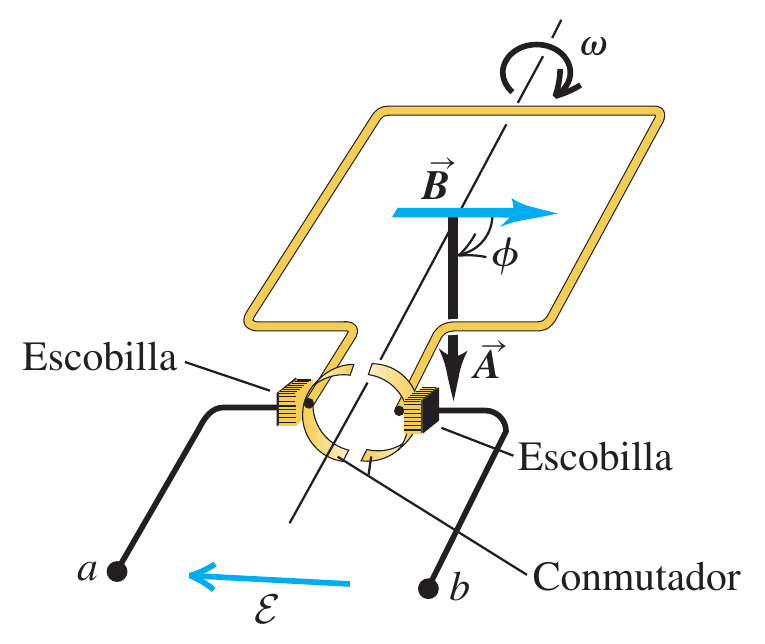
\includegraphics[scale=0.3]{preguntas-01.png}
  \captionof{figure}{Pregunta \ref{p:preguntasIV01}\label{f:preguntasIV01}}
\end{center}
%
\begin{Exercise}
    Dos espiras circulares se encuentran lado a lado en el mismo plano. Una está conectada a una fuente que suministra una corriente creciente; la otra es un anillo cerrado simple. ¿La corriente inducida en el anillo tiene el mismo sentido que la corriente en la espira conectada con la fuente o es opuesto? ¿Qué sucede si disminuye la corriente en la primera espira?
\end{Exercise}
%
\begin{Exercise}
    Un conductor largo y recto pasa por el centro de un anillo metálico, perpendicular a su plano. Si la corriente en el conductor aumenta, ¿se induce una corriente en el anillo?
\end{Exercise}
%
\begin{Exercise}
    Un estudiante asegura que, si se deja caer en forma vertical un imán permanente por un tubo de cobre, finalmente el imán alcanza una velocidad terminal, aunque no haya resistencia del aire. ¿Por qué tendría que ser así?
\end{Exercise}
%
\begin{Exercise}
    Un avión vuela horizontalmente sobre la Antártida, donde el campo magnético terrestre está dirigido mayormente hacia arriba alejándose del suelo. Vista por un pasajero que mira hacia el frente del avión, ¿el extremo del ala izquierda está a un potencial eléctrico mayor que el del ala derecha? ¿La respuesta depende de la dirección en que vuela el avión?
\end{Exercise}
%
\begin{Exercise}
    Un rectángulo de metal está cerca de un alambre largo, recto y que conduce corriente, con dos de sus lados paralelos al alambre. Si la corriente en el alambre está disminuyendo, ¿el rectángulo es repelido o atraído por el alambre? Explique por qué este resultado es congruente con la ley de Lenz.
\end{Exercise}
%
\begin{Exercise}\label{p:preguntasIV02}
    En la situación que se muestra en la figura \ref{f:preguntasIV02}, ¿sería adecuado preguntar cuánta energía gana un electrón durante un recorrido completo alrededor de la espira de alambre con corriente $I$? ¿Sería adecuado preguntar a través de qué diferencia de potencial se mueve el electrón durante ese recorrido completo?
\end{Exercise}
%
\begin{center}
    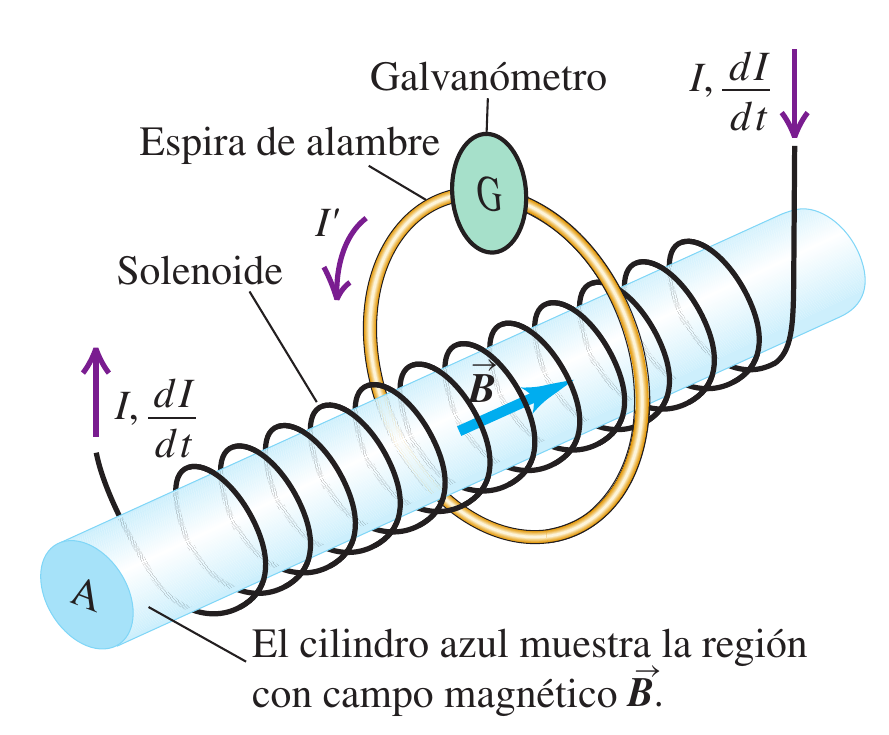
\includegraphics[scale=0.3]{preguntas-02.png}
    \captionof{figure}{Pregunta \ref{p:preguntasIV02}\label{f:preguntasIV02}}
\end{center}
%
\begin{Exercise}
    Una espira conductora cuadrada está en una región de campo magnético constante y uniforme. ¿La espira puede hacerse girar alrededor de un eje a lo largo de un lado sin que se induzca alguna fem en la espira? Explique lo que sucede en términos de la orientación del eje de rotación con respecto a la dirección del campo magnético.
\end{Exercise}
%
\begin{Exercise}
    Indique cuáles de los siguientes enunciados son verdaderos y justifique su elección.
    \begin{itemize}
        \item $\int\int \vec{B} \cdot d\vec{S} = 0 \Leftrightarrow \varepsilon_{ind} = 0$
        \item El signo negativo de la ley de Faraday es consecuencia del principio de acción y reacción.
        \item Un solenoide puede considerarse ideal si es muy largo.
        \item Una corriente variable no puede inducir una fem de valor constante.
        \item $\varepsilon_{ind} \neq 0 \Rightarrow \int\int \vec{B} \cdot d\vec{S} \neq 0$
        \item Una corriente estacionaria genera un campo magnético estacionario y no necesariamente uniforme.
        \item Una bobina almacena energía del campo eléctrico.
        \item La energía almacenada por una bobina es independiente del valor de la corriente que la circula.
        \item Un campo magnético variable siempre induce una f.e.m en toda espira sumergida en él.
        \item El campo magnético inducido es siempre opuesto al campo magnético externo.
        \item El signo negativo en la ley de Faraday-Lenz es consecuencia de la conservación de la energía.
    \end{itemize}
\end{Exercise}
%
\begin{Exercise}
    Para resistencias muy grandes, es fácil construir circuitos $RC$ que tengan constantes de tiempo de varios segundos o minutos. ¿Cómo se utilizaría este hecho para medir resistencias muy grandes, demasiado grandes como para medirlas con métodos más convencionales?
\end{Exercise}
%
\begin{Exercise}
    Cuando un capacitor, una batería y un resistor se conectan en serie, ¿el resistor afecta la carga máxima que se almacena en el capacitor? ¿Por qué? ¿Qué finalidad tiene el resistor?
\end{Exercise}
%
\begin{Exercise}\label{p:preguntasIV03}
    En el circuito mostrado en la figura \ref{f:preguntasIV03}, cuando se cierra el interruptor, el potencial $V_{ab}$ cambia súbitamente y en forma discontinua, a diferencia de la corriente. Explique por qué el voltaje puede cambiar de pronto, pero la corriente no.
\end{Exercise}
%
\begin{center}
\begin{circuitikz}[scale=1]
    \draw (0,1.5) to[R=$R$, color=red] (2.5,1.5) to[L, l=$L$, color=green!80!black] (5,1.5)
    (0,1.5) -- (0,3) to[battery2, color=cyan] (2.5,3) to[switch] (5,3) -- (5,1.5);
    \fill (0,1.5) circle (3pt) node [below] {$a$};
    \fill (2.5,1.5) circle (3pt) node [below] {$b$};
\end{circuitikz}
\captionof{figure}{Pregunta \ref{p:preguntasIV03}\label{f:preguntasIV03}}
\end{center}
%
\begin{Exercise}
    Suponga que hay una corriente estable en un inductor. Si trata de reducir la corriente a cero en forma instantánea abriendo rápidamente un interruptor, puede aparecer un arco donde el interruptor hace contacto. ¿Por qué? ¿Es físicamente posible detener la corriente de forma instantánea? Explique su respuesta.
\end{Exercise}
%

\twocolumn[\colorsection{Respuestas de la unidad IV}]
%   \begin{multicols*}{2}
    \shipoutAnswer
%   \end{multicols*}

  \end{document}